% !TeX spellcheck = en_US
\documentclass[12pt]{amsart}

\usepackage{answers}
\usepackage{setspace}
\usepackage{enumitem}
\usepackage{multicol}
\usepackage{mathrsfs}
\usepackage[margin=1in]{geometry} 
\usepackage{amsmath,amsthm,amssymb}
\usepackage{listings}
\usepackage{xspace}


\usepackage{amsfonts,amssymb,amsbsy}
\usepackage{latexsym}
\usepackage{color}
\usepackage{graphics} 
\usepackage{float}
\usepackage{subfigure}
\usepackage{epsfig} 
\usepackage{epstopdf}
\usepackage{caption}
\usepackage{longtable}
\usepackage{afterpage}
\usepackage{array,booktabs,enumitem}
\usepackage{algorithm}  
\usepackage{algorithmicx}  
\usepackage{algpseudocode}  
\usepackage{mathrsfs}
\usepackage{bm}
\usepackage{tikz}
\usepackage{hyperref}
\usepackage{cleveref}
\usepackage{multirow}
\newtheorem{theorem}{Theorem}[section]
\newtheorem{proposition}[theorem]{Proposition}
\newtheorem{lemma}[theorem]{Lemma}
\theoremstyle{definition}
\newtheorem{definition}[theorem]{Definition}
\theoremstyle{remark}
\newtheorem{remark}[theorem]{Remark}
\newtheorem{test}{Problem}
\newtheorem{example}{Example}

\newtheoremstyle{assumption}
  {6pt}
  {6pt}
  {\rm}
  {}
  {\bfseries}
  {}
  {1pt}
  {}
\theoremstyle{assumption}
\newtheorem{assumption}{Assumption} 
\def\theassumption{(A\arabic{assumption})}

\usepackage[colorinlistoftodos,bordercolor=orange,backgroundcolor=orange!20,linecolor=orange,textsize=scriptsize]{todonotes}
\usepackage{frenchineq}
\newcommand{\veryshortarrow}[1][3pt]{\mathrel{
   \hbox{\rule[\dimexpr\fontdimen22\textfont2-.2pt\relax]{#1}{.4pt}}
   \mkern-4mu\hbox{\usefont{U}{lasy}{m}{n}\symbol{41}}}}

\makeatletter

\setbox0\hbox{$\xdef\scriptratio{\strip@pt\dimexpr
    \numexpr(\sf@size*65536)/\f@size sp}$}

\newcommand{\scriptveryshortarrow}[1][3pt]{{
    \hbox{\rule[\scriptratio\dimexpr\fontdimen22\textfont2-.2pt\relax]
               {\scriptratio\dimexpr#1\relax}{\scriptratio\dimexpr.4pt\relax}}
   \mkern-4mu\hbox{\let\f@size\sf@size\usefont{U}{lasy}{m}{n}\symbol{41}}}}

\makeatother

\newcommand{\fromsource}{_{\mathrm{s}\veryshortarrow}}
\newcommand{\todest}{_{\veryshortarrow\mathrm{d}}}
\newcommand{\tox}{_{\veryshortarrow\mathrm{x}}}

\newcommand{\source}{x_{\textrm{src}}}
\newcommand{\dest}{x_{\textrm{dst}}}

\newcommand{\sourceset}{\mathcal{K}_{\textrm{src}}}
\newcommand{\destset}{\mathcal{K}_{\textrm{dst}}}

\newcommand{\optsourceset}{\mathcal{X}_{\textrm{src}}}
\newcommand{\optdestset}{\mathcal{X}_{\textrm{dst}}}

\newcommand{\Fine}{\text{\sc Fine}\xspace}
\newcommand{\Finegrid}{\text{\sc Fine-grid}\xspace}
\newcommand{\Coarsegrid}{\text{\sc Coarse-grid}\xspace}

\newcommand{\Far}{\text{\sc Far}\xspace}
\newcommand{\Accepted}{\text{\sc Accepted}\xspace }
\newcommand{\Narrow}{\text{\sc NarrowBand}\xspace } 
\newcommand{\Active}{\text{\sc Active}\xspace }
\newcommand{\Start}{\text{\sc Start}\xspace } 
\newcommand{\End}{\text{\sc End}\xspace } 

\newcommand{\lowerboundf}{\underline{f}}
\newcommand{\upperboundf}{\overline{f}}

\newcommand{\spacecom}{\mathcal{C}_{spa}}
\newcommand{\computcom}{\mathcal{C}_{comp}}
 
\newcommand{\N}{\mathbb{N}}
\newcommand{\Z}{\mathbb{Z}}
\newcommand{\C}{\mathbb{C}}
\newcommand{\R}{\mathbb{R}}
\newcommand{\A}{{\mathcal A}}
\newcommand{\I}{[I]}
\newcommand{\NL}{{\mathit L}}
\newcommand{\Omegab}{\overline{\Omega}}
\newcommand{\Rp}{\R_+}
\newcommand{\F}{{\mathcal F}}
\newcommand{\K}{{\mathcal K}}
\newcommand{\Cc}{{\mathcal C}}

\newcommand{\NEW}[1]{{\em #1}}

\newcommand{\Oc}{\mathcal{O}}
\newcommand{\gT}{\partial_{\mathrm t} \Oc}
\newcommand{\Oetab}{\overline{\mathcal{O}}_{\eta}}
\newcommand{\Oeta}{\mathcal{O}_{\eta}}

\newcommand{\Oetamu}{\mathcal{O}_{\eta}^\mu}
\newcommand{\Oetabmu}{\overline{\mathcal{O}_{\eta}^{\mu}}}

\DeclareMathOperator{\sech}{sech}
\DeclareMathOperator{\csch}{csch}


\newcommand{\etaH}{\eta_H}
\newcommand{\epsH}{\varepsilon_H}
\newcommand{\argmin}{\operatorname{Argmin}}



\makeatletter
\newenvironment{breakablealgorithm}
{
			\refstepcounter{algorithm}
			\hrule height.8pt depth0pt \kern2pt
			\renewcommand{\caption}[2][\relax]{
				{\raggedright\textbf{\ALG@name~\thealgorithm} ##2\par}
				\ifx\relax##1\relax 
				\addcontentsline{loa}{algorithm}{\protect\numberline{\thealgorithm}##2}
				\else 
				\addcontentsline{loa}{algorithm}{\protect\numberline{\thealgorithm}##1}
				\fi
				\kern2pt\hrule\kern2pt
			}
		}{
		\kern2pt\hrule\relax
}
\makeatother

\usepackage{geometry}


\renewcommand{\theenumi}{\roman{enumi}}
\renewcommand{\labelenumi}{\rm (\theenumi)}





\begin{document}
 
 
\title{A multi-level fast-marching method For The Minimum time problem 
}
 \date{\today} 
 
\author{Marianne Akian}
\author{St\'ephane Gaubert}
\address[Marianne Akian and St\'ephane Gaubert]{Inria and CMAP, \'Ecole polytechnique, IP Paris, CNRS}
\email{Marianne.Akian@inria.fr}
\email{Stephane.Gaubert@inria.fr}
\author{Shanqing Liu}
\address[Shanqing Liu]{CMAP, \'Ecole polytechnique, IP Paris, CNRS, and Inria}
\email{Shanqing.Liu@polytechnique.edu}
\begin{abstract}
	We introduce a new numerical method to approximate the solutions of a class of stationary Hamilton-Jacobi (HJ) partial differential equations arising from minimum time optimal control problems. We rely on several grid approximations, and look for the optimal trajectories by using
	the coarse grid approximations to reduce the search space 
	in fine grids.
	This may be thought of as an infinitesimal version of the ``highway hierarchy'' method which has been developed to solve shortest path problems
(with discrete time and discrete state).
	We obtain, for each level, an approximate value function on a sub-domain of the state space. We show that the sequence 
	obtained in this way does converge to the viscosity solution of the HJ equation.
Moreover, for our multi-level algorithm, if $0<\gamma \leq 1$ is the convergence rate of the classical numerical scheme, then the number of arithmetic operations needed to obtain an error in $O(\varepsilon)$ is in  $\widetilde{O}(\varepsilon^{-\frac{\theta d}{\gamma}})$, 
 to be compared with $\widetilde{O}(\varepsilon^{-\frac{d}{\gamma}})$ for ordinary grid-based methods.
Here $d$ is the dimension of the problem, and $\theta <1$ depends on 
$d$ and on the ``stiffness" of the value function around optimal trajectories, and the notation $\widetilde{O}$ ignores logarithmic factors. 
When  $\gamma =1$ and the stiffness is high, 
	this complexity becomes in $\widetilde{O}(\varepsilon^{-1})$. 
	We illustrate the approach by solving HJ equations of eikonal type up to dimension 7.
\end{abstract}


	
\maketitle
\section{Introduction}
\subsection{Motivation and context}
We consider a class of optimal control problems, consisting of finding the minimum traveling time between two given sets in a given domain.
 Such optimal control problems are associated to a stationary Hamilton-Jacobi (HJ) equation via the Bellman dynamic programming principle  (see for instance~\cite{flemingsoner}). In particular, the value function is characterized as the solution of the associated HJ equation in the viscosity sense~\cite{crandall1983viscosity,crandall1984some,flemingsoner}. Problems with state constraints can be addressed with the notion of constrained viscosity solution~\cite{soner1986optimal1,soner1986optimal2}. 

Various classes of numerical methods have be proposed to solve this problem. 
The \textit{Finite difference schemes} are based on a direct discretization of the HJ equation (see for example \cite{Crandall1984TwoAO}). The \textit{Semi-Lagrangian schemes}, as in \cite{falcone1987numerical,falcone2013semi}, arise by applying the Bellman dynamic programming principle to the discrete time optimal control problem obtained after an Euler time discretization of the dynamics. 
In both cases, the discretized system of equations can be interpreted as the dynamic programming equation of a stochastic optimal control problem \cite{kushner2001numerical} with discrete time and state space. More recently, max-plus based discretization schemes have been developed in \cite{fleming2000max,Mc2006,Mc2007,akian2008max}. These methods take advantage of the max-plus linearity of the Lax-Oleinik evolution operator of the HJ equation. They are based on a max-plus basis representation of the discretized value function, leading to a discrete time deterministic optimal control problem.    

Once a discretization is done, traditional numerical methods apply iterative steps to solve the discretized stationary HJ equation, for instance value iteration or policy iteration. At each step, the value function is computed in the {whole} discretization grid. 
In the particular case of the shortest path problem (with discrete time and state space), with a nonnegative cost function, one can obtain the solution of the stationary dynamic programming equation by Dijkstra's algorithm.
The fast marching method introduced by Sethian in~\cite{sethian1996fast} and by Tsitsiklis in~\cite{tsitsiklis1995efficient}  is based on that observation.
It can be seen as a variant of Dijkstra's algorithm for a monotone finite difference discretization of the HJ equation of some continuous time and state shortest path problem. 
It is called "single pass" because at every point of the discretization grid, the value is computed at most $k$ times, where $k$ is a bound not related to the discretization mesh. 
Such an approach was initially introduced to solve the front propagation problem, then extended to more general stationary Hamilton-Jacobi equations. It takes advantage of the property that the evolution of the region behind a ``propagation front'' is monotonely increasing, the so called the ``causality'' property. In  general, the fast marching method implemented in a $d$-dimensional grid with
$M$ points requires a number of arithmetic operations in the order of
$K_d M\log M$, in which the constant $K_d\in [2d,D^d]$ depends
on the type of discrete neighborhood that is considered
(and $D$ is the maximal diameter of neighborhoods).

Although the fast-marching 
is a fast, single pass, method, 
it remains a grid-based method, and hence still suffers from the "curse of dimensionality". 
Indeed, the size of nonlinear systems to be solved is exponential in the dimension $d$, making the numerical computation untractable even on modern computers. Several types of discretizations or representations have been developped recently to overcome the curse of dimensionality for HJ equations. One may cite the sparse grids approximations of Bokanowski, Garcke, Griebel and Klompmaker~\cite{zbMATH06176972}, or of Kang and Wilcox~\cite{Ka.Wi2017}, the tensor decompositions of Dolgov, Kalise and Kunisch \cite{zbMATH07364328} or of
Oster, Sallandt and Schneider \cite{zbMATH07547920},
the deep learning techniques applied by Nakamura-Zimmerer, Gong, and Kang \cite{zbMATH07364322} or by Darbon and Meng \cite{zbMATH07508503}.
In the case of structured problems, one may also cite the 
max-plus or tropical numerical method of McEneaney \cite{Mc2006,Mc2007},
see also~\cite{mceneaney2,Qu2013,Qu2014,Do2018} for further developments,
and the Hopf formula of Darbon and Osher \cite{zbMATH06626046}, 
see also \cite{Ch.Da.Os.Yi2019,Ki.Ma.He.Da.Os.Ch2018,zbMATH07336741}.


Another way to overcome the curse of dimensionality is to replace the general problem of solving the HJ equation by the one of computing the optimal trajectories between two given points. The latter problem can be solved, under some convexity assumptions, by the Pontryagin Maximum Principle approach~\cite{raymond1998pontryagin,raymond1999pontryagin, bergounioux1999pontryagin}, which is normally done by searching for the zero of a certain shooting function (the dimensionality of the systems to be solved for such a shooting method is normally $2d$). Another method is the stochastic dual dynamic programming (SDDP)~\cite{pereira1991multi,shapiro2011analysis,girardeau2015convergence}, in which the value function is approximated by a finite supremum of affine maps, and thus can be computed efficiently by linear programming solvers. In the absence of convexity assumptions, these methods may only lead to a local minimum. In that case, more recent methods consist in exploiting the structure of the problem, in order to reduce the set of possible trajectories among which the optimization is done. For instance, Alla, Falcone and Saluzzi \cite{alla2019efficient} (see also \cite{alla2020tree}) introduced a tree structure discretization, taking advantage of the Lipschitz continuity of the value function. Also, Bokanowski, Gammoudi, and Zidani \cite{bokanowski2022optimistic} introduced an adaptive discretization in the control space, which has shown to be efficient when the dimension of control space is low.  
\subsection{Contribution}
In this paper, we intend to find the optimal trajectories between two given sets, for the minimal time problem.
We develop 
an adaptive multi-level and causal discretization of the state space, leading to a new algorithm.

Our method is inspired by the recent development of the "Highway Hierarchies" algorithm~\cite{delling2006highway, sanders2012engineering} for the (discrete) shortest path problems. The latter algorithm accelerates the Dijkstra's algorithm,
to compute the shortest path between any two given points. It first performs a pre-processing computing ``highways'' in which the optimal paths should go through, then computing the shortest path between two given points using suc highways. The highways are themselves computed using a partial application of the Dijkstra's algorithm. By doing so, one can find the exact shortest path, as by using Dijkstra's algorithm, but in a much shorter time. 
However, the original highway hierarchy method is difficult to implement in the case of a discretized HJ equation, even when this equation is associated to a shortest path problem. Indeed regularity properties may prevent the existence of highways in an exact sense. Also the computation and storage complexity of the pre-processing procedure (computing highways) is equivalent to the one of Dijkstra's algorithm, making the highway hierarchy method being more suitable to problems in which numerous queries have to be solved quickly, on a fixed graph
(a typical use case is GPS path planning).

Our approach combines the idea of highway hierarchy with the one of multi-level
grids, in order to reduce the search space.
Indeed, we compute (approximate) ``highways'' by using a coarse grid. 
Then, we perform a fast marching in a finer grid, restricted to a neigborhood of the highways. This method is iterated, with finer and finer grids, and smaller
and smaller neighborhoods, untill the desired accuracy is reached.

We show that, by using our algorithm, the final approximation error is as good as the one obtained by discretizing directly the whole domain with the finest grid. 
Moreover, the number of  elementary operations and the size of the memory needed to get an error of $\varepsilon$
are considerably reduced. Indeed, 
recall that the number of arithmetic operations
of conventional grid-based methods
is in the order of  $\widetilde{O}(\varepsilon^{-\frac{d}{\gamma}}K_d)$,
where $d$ is the dimension of the problem, 
$0<\gamma\leq 1$ is the convergence rate of the classical fast marching method,
$K_d \in [2d,L^d]$ for some constant $L$ depending on the 
diameter of discrete neighborhoods,
and $\widetilde{O}(x)$ ignores the logarithmic factors.
For our multi-level method, with suitable parameters,
the number of arithmetic operations
is in the order of  $\widetilde{O}(C^d \varepsilon^{-\frac{1+(d-1)(1-\gamma \beta)}{\gamma}})$, 
where $C>1$ is a constant depending on the problem characteristics, 
and $0<\beta \leq 1$ measures the ``stiffness" of the value function around optimal trajectories.
Then, 
our complexity bound reduces to 
$\widetilde{O}(C^d\varepsilon^{-1}) $ when $\gamma = \beta = 1$. 
Hence, considering the dependence in $\varepsilon$ only, we reduce
the complexity bound from $\widetilde{O}(\varepsilon^{-\frac{d}{\gamma}})$ to 
$\widetilde{O}(\varepsilon^{-\frac{1+(d-1)(1-\gamma \beta)}{\gamma}})$.
Moreover, under some regularity
assumptions, the complexity bound becomes 
$\widetilde{O}(\varepsilon^{-1})$ and is thus of same order as for 
one dimensional problems.           

This paper is organized as follows: In \Cref{Pre}, we give some preliminary results on the HJ equation and the minimum time optimal control problem. In \Cref{sec-cotra}, we present our original idea from the continuous point of view, and give some results which will be useful to prove the correctness of our algorithm. In \Cref{sec-algo}, we present our algorithm, from the discretization method to the implementation. We also describe a specific data storage structure, with hashing techniques, which is essential to implement our algorithm in an efficient way. In \Cref{sec-conv}, we give the computational complexity of our new algorithm, by providing error bound. Finally, in \cref{sec-test}, we present numerical tests, for problems of dimension $2$ to $7$.

\section{Hamilton-Jacobi equation for the Minimum Time Problem} \label{Pre}

\subsection{The Minimum Time Problem }
Let $\Omega$ be an open, bounded domain in $\R^{d}$. Let $S_{1}$ be the unit sphere in $\R^{d}$, i.e., $S_{1} = \{ x \in \R^{d}, \| x\| =1  \} $ where $\|\cdot\|$ denotes the Euclidean norm.
Let $\mathcal{A} = \{ \alpha : \R_{\geq0} \mapsto S_{1} : \alpha(\cdot) \text{ is measurable} \}  $ denote the set of controls, every $\alpha \in \A$ is then the unit vector determining the direction of motion. 
We denote by $f$ the speed function, and assume the following basic regularity properties: 
\begin{assumption} \label{assp1}$ $
      \begin{enumerate}
      \item $f : \Omegab\times S_1 \mapsto \R_{>0}$  is continuous.	
      \item $f$ is bounded on $\Omegab\times S_1$, i.e., $\exists M_f >0$ s.t. $\|f(x,\alpha) \| \leq M_f$, $\forall x \in \Omegab, \forall \alpha \in S_1$.
      \item There exists constants $L_{f}, L_{f,\alpha}>0$ such that $ |f(x,\alpha) - f(x^{'},\alpha)| \leq L_{f}| x - x^{'} |, \forall \alpha \in S_1, \forall x, x^{'}\in \Omega$ and  $| f(x,\alpha) - f(x,\alpha^{'})| \leq L_{f,\alpha}|\alpha - \alpha^{'}|, \forall x \in \Omega, \forall \alpha, \alpha^{'} \in S_1$.
      \end{enumerate}
\end{assumption}

Let $\sourceset$ and $\destset$ be two disjoint compact subsets of $\Omega$ 
(called the \NEW{source} and the \NEW{destination} resp.).
Our goal is to find the minimum time necessary to travel from $\sourceset$ to $\destset$, and the optimal trajectories between $\sourceset$ and $\destset$, together with the optimal control $\alpha$. 

We intend to solve the following optimal control problem:
\begin{equation}\label{problem}
	\begin{aligned}
		&\inf \ \tau \geq 0\\
		&s.t. \left\{
			\begin{aligned}
				& \dot{y}(t) = f(y(t),\alpha(t))\alpha(t), \ \forall t\in[0,\tau] \enspace , \\
				& y(0)\in\sourceset, \ y(\tau)\in\destset \enspace, \\
				& y(t) \in \overline{\Omega}, \ \alpha(t) \in \A, \ \forall t \in [0,\tau] \enspace .
			\end{aligned} \right.
	\end{aligned}
\end{equation}

\subsection{HJ Equation for the Minimum Time Problem.} A well known sufficient and necessary optimality condition for the above problem is given by the Hamilton-Jacobi-Bellman equation, which is deduced from the dynamic programming principle. Indeed, one can consider the following controlled dynamical system: 
\begin{equation}
\label{dynmsys}
\left\{
	\begin{aligned}
    &\dot{y} (t) = f(y(t), \alpha(t)) \alpha(t), \ \forall t \geq 0 \ ,\\
	&y(0) = x \ .
	\end{aligned}
\right.
\end{equation}
We denote by $y_{\alpha}(x;t)$ the solution of the above dynamical system \eqref{dynmsys} with $\alpha \in \mathcal{A}$ 
and $y_\alpha(x;s) \in \overline{\Omega}$ for all $0\leq s \leq t$. More precisely, we restrict the set of control trajectories so that the state $y$ stays inside the domain $\overline{\Omega}$, i.e., we consider the following set of controls: 
\begin{equation}\label{controlset}
	\mathcal{A}_{\Omega,x} := \{ \alpha \in \mathcal{A} \ | \  y_\alpha(x;s) \in \overline{\Omega}, \text{ for all }  s \geq 0  \} \enspace,
\end{equation}
and we further assume $A_{\Omega,x} \neq \emptyset$. In other words, the structure of the control set $A_{\Omega,x}$ is adapted to the state constraint ``~$y\in \overline{\Omega}$~''. 
Let us define the cost functional by: 
\begin{equation}\label{cost-func}
J\todest(\alpha(\cdot),x) = \inf \{ \tau \geq 0\mid y_{\alpha}(x;\tau) \in \destset \} \enspace,
\end{equation}
 "$\todest$" means arrival to destination. The value function $T\todest : \bar{\Omega} \mapsto \R \cup \{+\infty\}$ is defined by 
\begin{equation}\label{Mintime}
T\todest(x) = \inf_{\alpha \in \mathcal{A}_{\Omega,x}} J\todest(\alpha(\cdot),x) \ . 
\end{equation}
Then, restricted to $\overline{\Omega \setminus \destset}$, $T\todest$ is a viscosity solution of the following state constrained Hamilton-Jacobi-Bellman equation: 
\begin{equation} \label{hjes1}
\left\{
\begin{aligned}
&-(\min_{\alpha \in S_1} \{ (\nabla T\todest(x) \cdot \alpha) f(x,\alpha) \} +1) =0, \enspace & x\in \Omega \setminus \destset \ ,\\
&-(\min_{\alpha \in S_1 } \{ (\nabla T\todest(x) \cdot \alpha) f(x,\alpha) \} +1) \geq 0, \enspace & x\in \partial\Omega  \ , \\
&T\todest(x) = 0 \enspace \enspace & x\in \partial \destset \ .
\end{aligned}
\right.
\end{equation}
Here, considering $F(x,r,p) =- \min_{\alpha \in S_1} \{ p \cdot f(x,\alpha)\alpha + 1 \}$, $\Oc=\Omega \setminus \destset$ and $\gT  = \partial\destset$, 
 we use the following definition  for 
the viscosity solution of the following state constrained HJ equation 
with continuous hamiltonian $F: \R^d\times \R\times \R^d\to \R$,
open bounded domain $\Oc\subset \R^d$, 
and ``target'' $\gT\subset \partial \Oc$: 
\begin{equation}\label{constrainHJ}
	\tag*{$SC(F,\Oc,\gT )$}
	\left\{
	\begin{aligned}
	& F(x, u(x), Du(x)) = 0, \enspace & x \in \Oc\ , \\
	&F(x, u(x), Du(x)) \geq 0, \enspace & x \in \partial\Oc\setminus(\gT)
 \ ,  \\
	&u(x) = 0, \enspace & x \in \gT \ .
	\end{aligned}
	\right.
	\end{equation}
When there is no target set, that is $\gT=\emptyset$,
the following definition corresponds to the one
introduced first by Soner in~\cite{soner1986optimal1}
(see also \cite{bardi2008optimal}), the case with a nonempty
closed target set $\gT$
is inspired by the results of \cite{capuzzo-lions}.
\begin{definition}[compare with \protect{\cite{soner1986optimal1,bardi2008optimal,capuzzo-lions}}]
\label{constraint_vis} 
	Let $u: \overline{\Oc} \to \R$ be continuous.
	\begin{enumerate}
		\item The function $u$ is a viscosity subsolution 
		of \eqref{constrainHJ} if 
		for every test function $\psi \in \Cc^{1}(\overline{\Oc} )$, for all local maximum points $x_0 \in \overline{\Oc}$ of the function $u-\psi$, we have: \[ \begin{cases} F(x_0,u(x_0),D\psi (x_0) ) \leq 0& \text{if}\; 
			x_0\in \Oc \enspace,\\
u(x_0)\leq 0 &\text{if}\; 
			x_0\in \gT \enspace.
		\end{cases}
		\]
		\item The function $u$ is a viscosity supersolution of \eqref{constrainHJ} if for every test function $\psi \in \Cc^{1}(\overline{\Oc})$, for all local minimum points $x_0 \in \overline{\Oc}$ of the function $u-\psi$, we have: 
		\[ \begin{cases} F(x_0,u(x_0),D\psi (x_0) ) \geq 0& \text{if}\; 
			x_0\not\in \gT \enspace,\\
u(x_0)\geq 0 &\text{otherwise.}
		\end{cases}
		\]
		\item The function $u$ is a viscosity solution of \eqref{constrainHJ} if and only if it is a viscosity subsolution and supersolution of \eqref{constrainHJ}.
	\end{enumerate}
\end{definition}

A basic method in the studies of the above system (see \cite{vladimirsky2006static}, \cite{bardi1989boundary}, \cite[Chapter-IV]{bardi2008optimal}) is the change of variable:
\begin{equation} \label{changevar}
	v\todest(x) = 1 - e^{-T\todest(x)} \enspace,
\end{equation}
which was first used by Kruzkov~\cite{kruvzkov1975generalized}. By doing so, $v\todest(x)$ is automatically bounded and Lipschitz continuous. Once $v\todest$ is computed, we can directly get the minimum time for $x$ by $T\todest(x) = - \log(1 - v\todest(x))$.  

In fact, consider a new control problem associated to the dynamical system \eqref{dynmsys}, and the discounted cost  functional defined by
\begin{equation}\label{disc-cost}
J\todest^{'}(\alpha (\cdot),x) = \inf \left\{ \int_{0}^{\tau} e^{-t} dt \mid \tau\geq 0 , \ y_{\alpha}(x;\tau) \in \destset  \right\} \enspace ,
\end{equation}
for $\alpha \in \mathcal{A}_{\Omega,x}$. Then, the value function $v$ of the control problem given by
\begin{equation}\label{value-disc}
v (x) = \inf_{\alpha \in \mathcal{A}_{\Omega,x}} J\todest^{'}(\alpha(\cdot),x)
\end{equation}
 coincides with $v\todest$ in \eqref{changevar}.
Let now 
\begin{equation}
\label{defF}
F(x,r,p) = -\min_{\alpha \in S_{1}} \{ p \cdot f(x,\alpha)\alpha + 1 - r \}
\enspace .\end{equation}
 This Hamiltonian corresponds to the new control problem {\rm (\ref{dynmsys},\ref{disc-cost},\ref{value-disc})}, and the restriction of the value function $v\todest$ to $\overline{\Omega \setminus \destset}$ is a viscosity solution of the state constrained HJ equation $SC(F,\Omega\setminus \destset , \partial\destset)$.
 
The uniqueness of the solution of Equation $SC(F,\Omega\setminus \destset , \partial\destset)$ in the viscosity sense and the equality of this solution with the value function need not hold if the boundary condition is not well defined. 
When the target set is empty,
Soner \cite{soner1986optimal1,soner1986optimal2} introduced sufficient conditions for the uniqueness of the viscosity solution
of \eqref{constrainHJ} and the equality with the corresponding value function.
One of these conditions involves the dynamics of the controlled process on 
$\partial \Oc$,
see \cite[(A3)]{soner1986optimal1}, which is automatically
satisfied when $F$ is as in \eqref{defF}, and $f$ satisfies \Cref{assp1}
with $\Oc$ instead of $\Omega$. 
Similar conditions are proposed in \cite{capuzzo-lions}.
We state below the result of \cite{capuzzo-lions}
with the remaining conditions, and for a general open bounded domain $\Oc$,
instead of $\Omega$, 
as we shall need such a result in the sequel.
\begin{theorem}[Corollary of \protect{\cite[Th.\ IX.1, IX.3 and X.2]{capuzzo-lions}, see also \cite{soner1986optimal1}}]\label{th_soner}
Let $\Oc$ be an open domain of $\R^d$, let 
$\gT\subset \partial \Oc$ be compact, and assume that
 $\partial \Oc\setminus \gT$ is of class $\Cc^1$.
Let $F$ be as in \eqref{defF} with $f$ satisfying \Cref{assp1}
with $\Oc$ instead of $\Omega$. 
Then the comparison principle holds for $SC(F,\Oc , \gT)$, i.e., any viscosity subsolution is upper bounded by any viscosity supersolution. In particular, the viscosity solution is unique. Moreover, it coincides with 
the value function $v\todest$
in \eqref{value-disc} of the optimal control problem with dynamics 
\eqref{dynmsys} and
criteria \eqref{disc-cost},
in which $\Omega$ and $\destset$ are replaced by $\Oc$ and $\gT$, respectively.
\end{theorem}

We should also mention the recent works of \cite{bokanowski2010reachability, bokanowski2011deterministic,hermosilla2018mayer} which characterized the value function of the state constrained problems without any
controllability assumptions.

Once $SC(F,\Omega\setminus \destset , \partial\destset)$ is solved, one can easily get the value of the original minimum time problem by computing the minimum of $v\todest(x)$ over $\sourceset$. We shall denote the set of minimum points by $\optsourceset$, i.e., 
\begin{equation}\label{valuetodest}
	\optsourceset =\argmin_{x \in \sourceset} v\todest(x) 
 \enspace.
	\end{equation}
Since $v\todest$ is continuous (by \Cref{th_soner}) and $\sourceset$ is compact,
we get that $\optsourceset$ is a nonempty compact set.

\subsection{HJ Equation in Reverse Direction.}\label{sec_reverse} We shall also use another equivalent optimality condition characterization for the minimum time problem \eqref{problem}, obtained by applying the dynamic programming principle in a reverse direction. 

Let us consider the following controlled dynamical system:
\begin{equation}
\label{dynmsys_t}
\left\{
	\begin{aligned}
    &\dot{\tilde{y} } (t) = -f(\tilde{y}(t), \tilde{\alpha}(t)) \tilde{\alpha}(t), \ \forall t \geq 0 \ ,\\
	&\tilde{y}(0) = x \ .
	\end{aligned}
\right.
\end{equation}
We denote by $\tilde{y}_{\tilde{\alpha}}(x;t)$ the solution of the above dynamical system \eqref{dynmsys_t} with $\tilde{\alpha}(t) = \alpha(\tau-t) \in \A$, for all $t\in[0,\tau]$. Then automatically $\tilde{y}(t) = y(\tau - t)$ with $y$ as in \eqref{dynmsys}. Let us denote the state constrained control trajectories for this new problem by $\tilde{\A}_{\Omega,x}$, i.e., 
\begin{equation}
	\tilde{\A}_{\Omega,x} = \{ \tilde{\alpha} \in \A \ | \ \tilde{y}_{\tilde{\alpha}}(x;s) \in \overline{\Omega}, \text{ for all } s \geq 0 \}\ .
\end{equation}
Consider the following cost functional:
\begin{equation}\label{cost_s}
	J\fromsource(\tilde{\alpha}(\cdot),x) = \inf\{ \tau \geq 0\mid \tilde{y}_{\tilde{\alpha}}(x;\tau) \in \sourceset \} \ ,
\end{equation}
where "$\fromsource$" means from source, and the value function is given by
\begin{equation}\label{time_s}
	T\fromsource(x) = \inf_{\tilde{\alpha}\in \tilde{\A}_{\Omega,x}} J\fromsource(\tilde{\alpha}(\cdot),x) \in \R \cup \{+\infty\} \ .
\end{equation}
Then, the restriction of $T\fromsource $ to $\overline{\Omega \setminus \sourceset}$ is a viscosity solution of the following state constrained HJ equation:
\begin{equation}\label{hjbt}
	\left\{
		\begin{aligned}
		&-(\min_{\alpha \in S_1} \{ -(\nabla T\fromsource(x) \cdot \tilde{\alpha}) f(x,\tilde{\alpha}) \} +1) =0, \enspace &x\in \Omega \setminus \sourceset \ ,\\
		&-(\min_{\alpha \in S_1 } \{ -(\nabla T\fromsource(x) \cdot \tilde{\alpha}) f(x,\tilde{\alpha}) \} +1) \geq 0, \enspace &x\in \partial\Omega \ , \\
		&T\fromsource(x) = 0 , \enspace &x \in \partial \sourceset \ .
		\end{aligned}
		\right.
\end{equation}	

Using the same change of variable technique, we have $v\fromsource(x) = 1 - e^{-T\fromsource(x)}$, and we transform the above system \eqref{hjbt} into the state constrained HJ equation $SC(F^*,\Omega\setminus\sourceset,\partial \sourceset)$, where $F^*(x,r,p) = F(x,r,-p)$. 
Notice that $SC(F^*,\Omega\setminus\sourceset,\partial \sourceset)$ is also associated to a new optimal control problem, for which the dynamics is given by \eqref{dynmsys_t} and the value function is given by 
\begin{equation}\label{value_s_v}
	v\fromsource(x) = \inf_{\tilde{\alpha}\in \tilde{\A}_{\Omega,x}} \inf \left\{ \int_{0}^{\tau} e^{-t} dt \mid \tau\geq 0,\ \tilde{y}_{\tilde{\alpha}}(x;\tau) \in \sourceset \right\} \ .
\end{equation}

By doing so, to solve the original minimum time problem \eqref{problem}, one can also solve the equation $SC(F^*,\Omega\setminus\sourceset,\partial \sourceset)$ to get $v\fromsource$, %to find $v\fromsource(\dest)$, 
and then compute the minimum of $v\fromsource(x)$ over $\destset$. We shall also denote by $\optdestset$ the set of minimum points, i.e.,
\begin{equation}\label{valuefromsource}
	 \optdestset = 
\argmin_{x \in \destset}  v\fromsource(x) 
\enspace.
	\end{equation}
Again, as for $\optsourceset$,  we get that $\optdestset$ 
 is a nonempty compact set.

\section{Reducing the State Space of the Continuous Space Problem}\label{sec-cotra}

The above two equivalent characterizations of the minimum time between $\sourceset$ and $\destset$ give us an inspiration to formulate optimal trajectories between $\sourceset$ and $\destset$ by using the value functions from the two directions.  In this section, we shall show how to reduce the state space $\Omega$ of the original minimum time problem, using $v\fromsource$ and $v\todest$, while preserving optimal trajectories. 
\subsection{The Optimal Trajectory}
We first give the definition of an optimal trajectory: 
\begin{definition}
	For every $x\in \Omegab$, 
	We say that $y_{\alpha^{*}}(x;\cdot):[0,\tau] \mapsto \Omegab$ is an optimal trajectory with associated optimal control $\alpha^{*}$ for Problem 
	{\rm (\ref{dynmsys},\ref{disc-cost},\ref{value-disc})}, if the minimum in \eqref{value-disc} is achieved in $\alpha^{*}$. We denote by $\Gamma^{*}_x$ the set of {\em geodesic points} starting from $x$, i.e., 
	$$\Gamma^{*}_x = \{ y_{\alpha^{*}}(x;t) \ | \ t\in[0,\tau] , \ {\alpha}^* \text{ optimal } \}\enspace.$$
\end{definition}
\begin{remark}
	We can use the same method to define the optimal trajectory for the problem in reverse direction as defined in \Cref{sec_reverse}. Moreover, we denote $\tilde{\Gamma}_x^{*}= \{ \tilde{y}_{\tilde{\alpha}^{*}}(x;t) \ | \ t \in [0,\tau], \ \tilde{\alpha}^* \text{ optimal } \}$ the set of geodesic points starting from $x$ in the reverse direction. 
\end{remark}

\begin{proposition}\label{geodesicpoints}
We have
	$$\cup_{x\in \optsourceset} \{ \Gamma^*_x \} = \cup_{x\in\optdestset} \{ \tilde{\Gamma}^*_x \}\enspace ,$$
and if the latter set is nonempty, then
$$ \inf_{x \in \sourceset} v\todest(x) = \inf_{x  \in \destset} v\fromsource(x)\enspace .$$
	\end{proposition}
\begin{proof}
	Let $y_{\alpha^*}(\source;\cdot) : [0,\tau^*] \mapsto \Omegab$  be an optimal trajectory for the problem {\rm (\ref{dynmsys},\ref{disc-cost},\ref{value-disc})}, with $\source \in \sourceset$ and the optimal control $\alpha^*$. Let us denote $\dest:=y_{\alpha^*}(\source;\tau^*)  \in \destset$. Consider the problem in reverse direction starting at $\dest$, and the control $\tilde{\alpha}^*$ such that $\tilde{\alpha}^*(s) = \alpha^*(\tau^* - s)$, $\forall s \in [0,\tau^*]$. Then, the associated state at time $s$ is $\tilde{y}_{\tilde{\alpha}^*}(\dest;s) = y_{\alpha^*}(\source;\tau^* -s)$. In particular $\tilde{y}_{\tilde{\alpha}^*}(\dest;\tau^*)  = \source \in \sourceset$, and
the trajectory $\tilde{y}_{\tilde{\alpha}^*}(\dest;\cdot)$ arrives in $\sourceset$ 
at time $\tau^*$. By definition of the value function, we have:
	\begin{equation}\label{value_2direction2}
		v\fromsource(\dest) \leq \int_{0}^{\tau^*} e^{-s}ds = v\todest (\source) \ ,
		\end{equation} 
with equality if and only if $\tilde{\alpha}^*$ is optimal.

Let us assume that $\cup_{x\in \optsourceset} \{ \Gamma^*_x \}$ is nonempty, 
and take $\source \in \optsourceset$, such that $\Gamma^*_{\source}$ is
nonempty, we get 
	\begin{equation}\label{value_2direction}
		v\fromsource(\dest) \leq v\todest(\source)=\inf_{\source \in \sourceset} v\todest(\source) \ .
		\end{equation}
If the above inequality is strict, then there exists
a trajectory (not necessary optimal)
$\tilde{y}_{\tilde{\alpha}'}(\dest;\cdot)$  starting from $\dest$ and arriving
in $\source'\in\sourceset$ at time $\tau'< \tau^*$.
Then, the reverse trajectory $y_{\alpha'}(\source';\cdot)$ 
is starting from $\source'$ and arrives in $\dest$ at time $\tau'$,
and we get $v\todest(\source')= 1-e^{-\tau'}< v\todest(\source)$ which is 
impossible.
This shows the equality in \eqref{value_2direction} and that 
$\tilde{\alpha}^*$ is optimal, so $\tilde{\Gamma}^*_{\dest}$ is nonempty.
Also, if $\dest\notin\optdestset$,
 by the same construction applied to $\dest'\in \optdestset$,
we get a contradiction, showing that $\dest\in\optdestset$.
Hence $\cup_{x\in\optdestset} \{ \tilde{\Gamma}^*_x \}$ is nonempty,
and 
$y_{\alpha^*}(\source;s) =  \tilde{y}_{\tilde{\alpha}^*}(\dest;\tau^*-s)  \in  
\cup_{x\in\optdestset} \{ \tilde{\Gamma}^*_x\} . $ 
Since this holds for all optimal trajectories $y_{\alpha^*}$ starting in
any $\source \in \optsourceset$, we deduce that
$\cup_{x\in \optsourceset} \{ \Gamma^*_x \}\subset  \cup_{x\in\optdestset} \{ \tilde{\Gamma}^*_x \}$.
By symmetry, we obtain the equality, so the first equality of
the proposition.
Moreover, by the equality in \eqref{value_2direction}, 
we also get the second equality of the proposition. 
	\end{proof} 
\begin{remark}\label{regeo}
Note that in \Cref{geodesicpoints}, all the sets $\Gamma^*_x$
with $x\in \optsourceset$ may be empty,
which would imply that all the sets $\tilde{\Gamma}^*_x$ with $x\in\optdestset$
are empty. 
In that case, we need to replace the sets $\Gamma^*_x$ and $\tilde{\Gamma}^*_x$
by $\delta$-geodesic sets.
	\end{remark}
From now on,
 we set $\Gamma^* =\cup_{x\in \optsourceset} \{ \Gamma^*_x \} = \cup_{x\in\optdestset} \{ \tilde{\Gamma}^*_x \} $, and call it \NEW{the set of geodesic points from $\sourceset$ to $\destset$}.
When $\Gamma^*$ is nonempty, using \Cref{geodesicpoints},
we shall denote by $v^*$ the following value:
\[ 
v^*:=\inf_{x \in \sourceset} v\todest(x) = \inf_{x 	\in \destset} v\fromsource(x)
\enspace . \] 
Once $v^*$ is obtained, we can directly get the minimum time by $\tau^* = -\log(1-v^*)$.

\begin{lemma}\label{pro-tra} Assume $\Gamma^{*}$ is non-empty. Then, we have 
\begin{equation}\label{opt-traj}
v^*= \inf_{y \in \Omegab} \{v\fromsource (y) + v\todest(y) - v\fromsource(y) v\todest(y) \}\enspace ,
\end{equation}
and the infimum is attained for every $x \in \Gamma^{*}$. 
Moreover, if there exists an optimal trajectory between any two points of $\Omegab$, then $x$ is optimal in 
\eqref{opt-traj}, that is $(v\fromsource(x) + v\todest(x) - v\fromsource(x)v\todest(x) ) = v^*$, if and only if $x \in \Gamma^{*}$.
\end{lemma}
\begin{proof}
Fix $x \in \Omegab$.  By definition of the value function, we have:
\begin{equation*}
v\fromsource(x)=  \inf \limits_{\tau>0,\tilde{\alpha}\in {\tilde{\A}}_{\Omega,x}\atop \tilde{y}_{\tilde{\alpha}} (x;\tau) \in \sourceset }  \left\{ \int_{0}^{\tau} e^{-t} dt  \right\}, \enspace
 v\todest(x) = \inf_{\tau'>0,\alpha'\in {\mathcal A}_{\Omega,x} \atop  y_{\alpha'} (x;\tau^{'}) \in \destset } \left\{ \int_{0}^{\tau^{'}} e^{-t} dt  \right\} \enspace .
\end{equation*}
For any $\tau>0$ and $\tilde{\alpha}\in {\tilde{\A}}_{\Omega,x}$ s.t.\ $\tilde{y}_{\tilde{\alpha}} (x;\tau) \in \sourceset$, denote $ \source = \tilde{y}_{\tilde{\alpha}} (x;\tau) \in \sourceset$. Then, by the simple change of variable $s = \tau -t$ and $\alpha(s)=\tilde{\alpha}(\tau-t)$, we have $\alpha \in \A_{\Omega,\source}$ and $y_{\alpha}(\source;\tau)=x$. This implies 
\begin{equation}\label{value_xfroms}
 v\fromsource(x) = \inf \limits_{\tau >0, \source \in \sourceset, \alpha \in \A_{\Omega,\source} \atop y_{\alpha}(\source;\tau)=x} \left\{ \int_{0}^{\tau} e^{-s} ds \right\} \enspace .
\end{equation}
Moreover, for $\tau'>0$ and $\alpha'\in {\mathcal A}_{\Omega,x}$ s.t.\ $y_{\alpha'} (x;\tau^{'}) \in \destset$, we denote $\dest = y_{\alpha'} (x;\tau^{'}) \in \destset$, so that
\begin{equation}\label{value_xtodest}
 v\todest(x) = \inf_{\tau'>0, \dest\in  \destset, \alpha'\in {\mathcal A}_{\Omega,x} \atop  y_{\alpha'} (x;\tau^{'}) = \dest } \left\{ \int_{0}^{\tau^{'}} e^{-t} dt  \right\} \enspace .
\end{equation}
Let $\tau >0, \source \in \sourceset, \alpha \in \A_{\Omega,\source}$ be such that
$y_{\alpha}(\source;\tau)=x$ and $\tau'>0, \dest\in  \destset, \alpha'\in {\mathcal A}_{\Omega,x}$ be such that $ y_{\alpha'} (x;\tau^{'}) = \dest$.
Concatenating $\alpha$ stopped at time $\tau$ and $t\in [\tau,\infty)\mapsto \alpha'(t-\tau)$, we obtain $\alpha''\in {\mathcal A}_{\Omega,\source}$
such that $y_{\alpha''}(\source;\tau+\tau')=\dest$  and
the trajectory from $\source$ to $\dest$ is going through $x$ at time $\tau$. 
Then, 
\begin{equation}\label{sumoftau}
 \int_{0}^{\tau} e^{-s}ds + e^{-\tau} \int_{0}^{\tau^{'}} e^{-t} dt =\int_{0}^{\tau+\tau'} e^{-s}ds \geq v^*\enspace .\end{equation}
where the last inequality  comes from the second
equality in \Cref{geodesicpoints}.

For any $\lambda, \mu\in [0,1]$, rewriting 
$\lambda+\mu-\lambda\mu= \lambda+ (1-\lambda) \mu$ or $\mu+(1-\mu)\lambda$, we see that the map $[0,1]^2\to \R, \; (\lambda,\mu)\mapsto \lambda+\mu-\lambda\mu$ is nondecreasing in each of its variables (separately), and thus commutes with the infimum operation in each variable.
Using this property, and that $0\leq \int_{0}^{\tau} e^{-s} ds\leq 1$ and $1-  \int_{0}^{\tau} e^{-s} ds=e^{-\tau}$, for all $\tau>0$, and taking the infimum in
\eqref{sumoftau}, first over $\tau$ and then over $\tau'$, we deduce: 
\begin{equation*}
v\fromsource(x) + v\todest(x) - v\fromsource(x)v\todest(x)\geq v^*\enspace . 
	\end{equation*} 
Since the above inequality is an equality for $x\in\optdestset$ or $x\in\optsourceset$, we deduce \eqref{opt-traj}.

If $x \in \Gamma^{*}$, there exist $\source\in\sourceset$, $\dest\in\destset$ and $\alpha\in {\mathcal A}_{\Omega,\source}$ such that $y_{\alpha}(\source;\tau^{*})=\dest$ and $y_{\alpha}(\source;\tau) = x$ for some $0\leq \tau\leq \tau^*$. 
Taking $\tau'=\tau^*-\tau$, we get an equality in \eqref{sumoftau},
and using the nondecreasing property with respect to $\tau$ and $\tau'$,
we deduce the reverse inequality
$v^*\geq v\fromsource(x) + v\todest(x) - v\fromsource(x)v\todest(x)$, so the equality. 

Let now $x\in \Omega$ be optimal in \eqref{opt-traj}, that is satisfy $(v\fromsource(x) + v\todest(x) - v\fromsource(x)v\todest(x) ) = v^*$.
Assuming that there exists an optimal trajectory for each of the two minimum time problems starting from any point, 
 there exist $\tau >0, \source \in \sourceset, \alpha \in \A_{\Omega,\source}$ such that $y_{\alpha}(\source;\tau)=x$ and $\tau'>0, \dest\in  \destset, \alpha'\in {\mathcal A}_{\Omega,x}$ such that $ y_{\alpha'} (x;\tau^{'}) = \dest$,
which are optimal in the above infimum \eqref{value_xfroms} and \eqref{value_xtodest}.
So again concatenating $\alpha$ stopped at time $\tau=T\fromsource(x)$ and $t\in [\tau,\infty)\mapsto \alpha'(t-\tau)$, we obtain $\alpha''\in {\mathcal A}_{\Omega,\source}$ and
a trajectory from $\source$ to $\dest$ going through $x$ at time $\tau$ and arriving
at $\dest$ at time $\tau+\tau'$.
Using \eqref{sumoftau}, we get 
$v^*=(v\fromsource(x) + v\todest(x) - v\fromsource(x)v\todest(x) ) = 
\int_{0}^{\tau+\tau'} e^{-s}ds $, so $\alpha''$ is optimal, which shows 
$x\in \Gamma^*$.
\end{proof}

For easy expression, for every 
$x\in \overline{\Omega}$ and $v = (v\fromsource, v\todest)$, we denote
\begin{equation}\label{operF}
	\F_v(x) = v\fromsource(x) + v\todest(x) - v\fromsource(x) v\todest(x) \enspace.
\end{equation}

\subsection{Reduction of The State Space}
Let us now consider the open subdomain $\mathcal{O}_{\eta}$ of $\Omega$, 
determined by a parameter $\eta > 0$, and defined as follows:
\begin{equation} \label{eqo}
	\Oeta = \{ x\in (\Omega \setminus ( \sourceset \cup \destset) )  \ | \ \F_v(x) < \inf_{y \in \Omega} \{ \F_v(y) + \eta \} \ \} \enspace.
\end{equation}

By \Cref{assp1}, we observe that $v\fromsource$, $v\todest$ are continuous in $\overline{\Omega}$, so does $\F_v$, thus the infimum in \eqref{eqo} is achieved by an element $y\in \overline{\Omega}$, and by \Cref{pro-tra}, it is equal to $v^*+\eta$.
This also implies that $\Oeta$ is an open set. 
Since $\eta>0$, we also have that $\Oeta$ is always nonempty.
\begin{proposition}\label{newboundary} Under \Cref{assp1}, 
and assuming that $\Gamma^*$ is nonempty, we have
\[\optsourceset \subseteq (\partial \Oeta) \cap (\partial \sourceset),  \ \optdestset \subseteq (\partial \Oeta) \cap (\partial \destset), 
\; \text{and}\;\Gamma^* \subset \Oetab \quad \forall \eta > 0 \ . \] 
	\end{proposition}
\begin{proof}
Let us first notice that,  since $\F_v$ is continuous,
we have $\Oetab \supseteq \{ x\in \overline{(\Omega\setminus (\sourceset \cup \destset) )}  \mid \F_v(x) <  \inf_{y \in \Omega} \{ \F_v(y) + \eta \}$. Moreover, since 
$\sourceset$ and $\destset$ are disjoint compact subsets of $\Omega$,
then  $\partial \Oeta \supseteq \{ x\in \partial\Omega\cup\partial\sourceset \cup \partial \destset   \ | \ \F_v(x) <  \inf_{y \in \Omega} \{ \F_v(y) + \eta \}$.

	By the dynamic programming principle, and since the cost in
\eqref{cost_s} is $1$ (so positive),
and $\sourceset$ and $\destset$ are disjoint,
we have 
	\[ v\todest (x) > \inf_{y \in \partial \sourceset} v \todest(y)\, ,\]
for all $x$ in the interior of $\sourceset$ (any trajectory starting in
$x$ need to go through $\partial \sourceset$).
This implies that $\Gamma^*$ does not intersects the interior of $\sourceset$, 
and similarly  $\Gamma^*$ does not intersects the interior of $\destset$,
so
$\Gamma^*\subseteq \overline{(\Omega\setminus (\sourceset \cup \destset) )}$.
Moreover, $\optsourceset \subseteq \sourceset\cap \Gamma^* \subseteq \partial \sourceset$ and $\optdestset \subseteq \destset\cap \Gamma^* \subseteq \partial \destset$.

Now for all $x\in \Gamma^*$, we have $\F_v(x) = v^* = \inf_{y\in \Omegab} \F_v(y),$
so $x\in \Oetab$, showing that $\Gamma^*\subseteq  \Oetab$. 
Let us now take $x\in \optsourceset$. We already shown that
$\optsourceset \subseteq \partial \sourceset$,
and we also have $\optsourceset\subset \Gamma^*$,
so $\F_v(x) = v^*$. All together, this  implies that 
The same argument holds for $\optdestset$. 
	\end{proof}

To apply the comparison principle (\Cref{th_soner}), we need to work with
a domain with a $\Cc^1$ boundary. To this end, we assume the following assumption
\begin{assumption}\label{assump_trajec}
	Assume that $\Gamma^*$ is nonempty and that $\Gamma^* \subset \Omega$.
	\end{assumption}
Then, for every $\mu >0$,
we select a function $\F^\mu_v : \Omegab \to \R$, that is $\Cc^d$, and that approximates $\F$, i.e.,
\begin{equation}\label{F_regu}
	\| \F^\mu_v -\F_v \|_\infty < \mu \enspace . 
	\end{equation}
Let us also consider a domain $\Oeta^\mu$, deduced from $\F^\mu_v$ and defined as follows:
\begin{equation}\label{Oeta_regu}
	\Oeta^\mu = \{ x\in (\Omega \setminus (\sourceset \cup \destset)) \mid  \F^\mu_v (x) < \inf_{y \in \Omega} \{ \F_v (y) + \eta  \} \ \} \ , 
	\end{equation}
with $\mu < \eta$. We notice that $ \mathcal{O}_{\eta - \mu}^\mu \subseteq \Oeta \subseteq \mathcal{O}_{\eta+\mu}^\mu$ with arbitrary small $\mu$. 
Moreover $\overline{\Oeta^\mu}\subset \Omega$, for  $\eta$ and $\mu$
small enough.
Then, $\Oeta^\mu$ can be compared with $\Oeta$, and it is 
the strict sublevel set of the $\Cc^d$ function. It can then be 
seen as a regularization of $\Oeta$. 
So, for almost all $\eta$ (small enough) and $\mu$ small enough,
 $(\partial \Oeta^\mu) \setminus (\destset\cup 
 \sourceset)$ is $\Cc^1$ (Corollary of Morse-Sard Theorem, see~\cite{morse1939behavior,sard1942measure}). 

We shall see that $\mathcal{O}_\eta^\mu$ is a smooth neighborhood of optimal trajectories, and we intend to reduce the state space of our optimal control problem from $\Omegab$ to the closure $\Oetabmu$ of $\Oetamu$.  More precisely, starting with the problem in direction ``to destination'', we consider a new optimal control problem with the same dynamics and cost functional as in Problem {\rm (\ref{dynmsys},\ref{disc-cost},\ref{value-disc})}, but we restrict the controls so that the state $y(s)$ stays inside the domain $\Oetabmu$, $\forall s\geq0$. 

The reduction of the state space leads to a new set of controls:
\begin{equation}\label{controlseto}
	\mathcal{A}_{\eta,x} := \{\alpha \in \mathcal{A} \ | \ y_\alpha(x;s) \in \Oetabmu, \text{ for all }  s \geq 0 \} \enspace .
\end{equation}
Let $v\todest^{\eta}(x)$ denote the value function of the optimal control problem when the set of controls is $\mathcal{A}_{\eta,x}$. Consider a new state constrained HJ equation: $ SC(F,\Oetamu, (\partial \Oetamu) \cap (\partial \destset ))$, 
we have the following result:

\begin{proposition}[Corollary of~\Cref{th_soner}]
The value function $v\todest^{\eta}$ of the control problem in $\Oetabmu$ is the unique viscosity solution of $ SC(F,\Oetamu, (\partial \Oetamu) \cap (\partial \destset ))$. 
\end{proposition}
\begin{remark}
The same reduction works for the problem in the reverse direction, which is the problem in the direction "from source". 
We denote $v^{\eta}\fromsource$ the value function of this problem with the set of controls be $\tilde{\A}_{\eta, x} :=\{ \tilde{\alpha} \in \A \mid \tilde{y}_{\tilde{\alpha}} (x;s) \in \Oetabmu, \text{ for all } s \geq 0 \}  $.
\end{remark} 
By the above construction of $\Oetamu$, we have the following relation between the value function of the original problem and the value function of the reduced problem:

\begin{proposition}\label{lemmatra} 
	If $\ \Gamma^{*}$ is not empty, then $\Gamma^{*} \subseteq \Oetabmu $, and for all $x \in \Gamma^{*}$, we have: $$v\fromsource (x) = v\fromsource^{\eta} (x), \ v\todest(x) = v\todest^{\eta} (x) \ .$$ 
\end{proposition}
\begin{proof} $\Gamma^* \subseteq \Oetabmu$ is a straightforward result of \Cref{newboundary}. Then, we have $v\fromsource(x) \leq v\fromsource^\eta(x), v\todest (x)\leq v\todest^\eta(x)$ for all $x\in \Oetamu$, since $\Oetamu \subseteq \Omega$.
Then, we also have $v\fromsource(x) \geq v\fromsource^\eta(x), v\todest (x)\geq v\todest^\eta(x)$ for all $x\in \Gamma^*$, since there exists optimal trajectories from $x\in \Gamma^*$ staying in $\Gamma^*$ and $\Gamma^* \subseteq \Oetabmu$. 
\end{proof}	

\subsection{$\delta$-optimal trajectories and the value function}
The above results express properties of exact optimal trajectories. We will also consider
approximate, $\delta-$optimal, trajectories. We first give the definition of the $\delta-$optimal trajectory.
\begin{definition}
	For every $x\in \Omega$, we say $y_{\alpha^{\delta}}(x;\cdot):[0,\tau] \to \Omegab$ is a $\delta-$optimal trajectory with associated $\delta$-optimal control $\alpha^{\delta}:[0,\tau] \to S^1$ for the problem {\rm (\ref{dynmsys},\ref{disc-cost},\ref{value-disc})} if :
	\[
\ y_{\alpha^{\delta}}(x;\tau) \in \destset\quad\text{and}\quad \int_{0}^{\tau} e^{-t} dt  \leq v\todest(x) + \delta \enspace.
	\]
	We denote by $\Gamma^{\delta}_x$ the set of $\delta-$geodesic points starting from $x$, i.e., 
	\[\Gamma^{\delta}_x = \{ y_{\alpha^{\delta}}(x;t) \ | \ t\in[0,\tau], \ \alpha^\delta :[0,\tau] \to S^1\text{ $\delta$-optimal }\} \ .\]
	We define analogously $\delta$-optimal trajectories for the problem in reverse direction, and denote by $\tilde{\Gamma}^{\delta}_x$ the set of $\delta$-geodesic points starting from $x$ in the reverse direction. 
\end{definition}

Following the same argument as in \Cref{geodesicpoints}, we have the following result: 
\begin{proposition}\label{delta_geodesic}
	Let us denote
	\[ \optsourceset^\delta = \{ x \in \partial \sourceset \mid v\todest(x) \leq v^* +\delta \}, \ \optdestset^\delta = \{x \in \partial \destset \mid v\fromsource(x) \leq v^* + \delta \} \ , \]
	then we have: 
	\begin{equation}\label{delta_geoset}
\cup_{\delta'\in [0,\delta]}
	\cup_{x\in \optsourceset^{\delta-\delta'}} \{ \Gamma^{\delta'}_x \} = \cup_{\delta'\in [0,\delta]} \cup_{x\in \optdestset^{\delta-\delta'}} \{ \tilde{\Gamma}^{\delta'}_x \}.
	\end{equation}
\qed
	\end{proposition}
Let us denote the set in \eqref{delta_geoset} by $\Gamma^\delta$, and call it  \NEW{the set of $\delta-$geodesic points from $\sourceset$ to $\destset$}. In the following, we intend to deduce the relationship between $\Gamma^\delta$ and our $\eta-$neighborhood, $\Oeta$. Let us start with a property of the $\delta-$optimal trajectories.


\begin{lemma}\label{delta-programming}
	Let $y_{\alpha^{\delta}}(x;\cdot):[0,\tau_x^{\delta}]\to\Omegab$ be a $\delta-$optimal trajectory of Problem {\rm (\ref{dynmsys},\ref{disc-cost},\ref{value-disc})} with associated $\delta$-optimal control $\alpha^{\delta}$ and $\delta$-optimal time $\tau^{\delta}_x$. Assume $v\todest(x)<1$, i.e., the minimum time from $x$ to $\destset : \tau_x < + \infty$. For every $z = y_{\alpha^{\delta}}(x;t_z)$, let us define a control $\alpha': [0, \tau^\delta_x - t_z] \to S_1$ such that $ \alpha'(s) = \alpha^{\delta}(s+t_z), \forall s \in [0,\tau^\delta_x-t_z]$. Then, the associated trajectory starting in $z$ with control $\alpha'$, $y_{\alpha'}(z;\cdot):[0,\tau_x^{\delta}-t_z] \to \Omegab$, is at least $(e^{t_z}\delta)$-optimal for the problem {\rm (\ref{dynmsys},\ref{disc-cost},\ref{value-disc})} with initial state $z$. 
\end{lemma}
\begin{proof}
	By definition, we have $y_{\alpha^{\delta}}(x;\tau^{\delta}_x) \in \destset $,
and $\int_{0}^{\tau^{\delta}_x} e^{-t}dt \leq v\todest(x) + \delta. $ Then, considering the control $\alpha'$ defined above, we have $y_{\alpha'}(z;\tau_x^{\delta}-t_z) \in \destset$ and 
		\[ e^{-t_z} \int_{0}^{\tau_x^{\delta}-t_z} e^{-s} ds \leq v\todest(x) - \int_{0}^{t_z}e^{-s}ds + \delta \ .\]
By dynamic programming equation, we have
\[ v\todest(x)\leq \int_{0}^{t_z}e^{-s}ds +e^{-t_z} v\todest(z)\enspace ,\]
 which implies
		\[ \int_{0}^{\tau_x^{\delta}-t_z} e^{-s} ds 
\leq v\todest(z) + e^{t_z} \delta \ . \]
	We deduce the result from the definition of $(e^{t_z}\delta)$-optimal 
trajectories.
\end{proof}
\begin{remark}
	One can deduce the same result for the $\delta-$optimal trajectory of the problem in reverse direction. In fact, for the minimum time problem, our definition of the $\delta-$optimal trajectory implies $\tau^{\delta}_x - \tau^{*}_x \leq e^{\tau^{*}_x} \delta$, where $\tau^{\delta}_x$ and $\tau^{*}_x$ denote the $\delta-$optimal time and the true optimal time respectively.
\end{remark}

\begin{lemma}\label{delta-tra}
	For every $\eta > \delta >0$, we have $\Gamma^{\delta}\subseteq \Oetab $ .
\end{lemma}

\begin{proof}
	Let $y_{\alpha^{\delta'}}(\source;\cdot):[0,\tau] \to \Omegab$ denote  a $\delta'-$optimal trajectory for the problem  {\rm (\ref{dynmsys},\ref{disc-cost},\ref{value-disc})} with $\source \in \optsourceset^{\delta-\delta'}$ and $\delta'\leq \delta$, then 
we have $\dest:=y_{\alpha^{\delta}}(\source;\tau) \in \destset$, and
\[ 	\int_{0}^{\tau} e^{-s} ds\leq v\todest(\source)+\delta'\leq v^*+\delta\enspace .\]
It is sufficient to show that $y_{\alpha^{\delta'}}(\source;t_x) \in \Oetab$ for every $t_x \in [0,\tau]$. 
	
	For an arbitrary $t_x\in[0,\tau]$, let us denote $x:=y_{\alpha^{\delta'}}(\source;t_x)$. Let $\alpha': [0, \tau -t_x] \to S_1 $ be a control such that $ \alpha'(s) = \alpha^{\delta'}(s+t_x), \forall s \in [0,\tau-t_x]$. Then, we have that the associated trajectory starting at $x$ with control $\alpha'$, $y_{\alpha'}(x;\cdot):[0,\tau-t_x] \to \Omegab$ satisfies $y_{\alpha'}(x;s) = y_{\alpha^{\delta'}}(\source; s+t_x)$, for every $s\in[0,\tau-t_x]$. Then, 
 $$
 \begin{aligned}
	\int_{0}^{\tau} e^{-s} ds  
	 = 1 - \Big(1 -  \int_{0}^{t_x} e^{-s} ds\Big) \Big( 1 -\int_{0}^{\tau-t_x} e^{-s} ds\Big) \ .
 \end{aligned}
$$ 
By the definition of 
$v\todest$, and since $y_{\alpha'}(x;\tau-t_x) = \dest\in \destset$,
we have 
$ v\todest (x) \leq  \int_{0}^{\tau-t_x} e^{-s} ds $. 
Similarly, using the simple change of variable $s = t_x - s'$, we have
$v\fromsource(x) \leq \int_{0}^{t_x} e^{-s} ds $. Then we deduce:
$$
\begin{aligned}
&1 - \Big(1 -  \int_{0}^{t_x} e^{-s} ds\Big) \Big( 1 -  \int_{0}^{\tau-t_x} e^{-s} ds \Big) \\
 & \quad \geq 1 - (1 - v\fromsource(x)) (1 - v\todest(x)) = v\fromsource(x) + v\todest(x) - v\fromsource(x) v\todest(x) \enspace,
\end{aligned}
$$ 
and so $$
\begin{aligned} v\fromsource(x) + v\todest(x) - v\fromsource(x) v\todest(x ) &\leq v^* + \delta \enspace . 
\end{aligned}  $$
Using 
 \Cref{pro-tra}, and $\eta>\delta$,  we obtain that $x=y_{\alpha^{\delta}}(\source;t_x) \in \Oetab$ for all $t_x \in [0,\tau]$.
Since this is true for all $0\leq \delta'\leq \delta$, we obtain $\Gamma^{\delta}   \subseteq \Oetab$.
\end{proof}

\begin{lemma}
	For every $\delta^{'}>0$, we have $\mathcal{O}_{\eta} \subset \Gamma^{\eta+\delta'} $. 
\end{lemma}
\begin{proof}
	Take a $x\in \mathcal{O}_{\eta}$, it is sufficient to show that there exists at least one $(\eta+\delta^{'})-$optimal trajectory from $\sourceset$ to $\destset$ 
	that passes through $x$.

	Suppose there exist an optimal trajectory from  $x$ to $\sourceset$, and an optimal trajectory from $x$ to $\destset$, then,  concatenating the reverse trajectory of the optimal trajectory from  $x$ to $\sourceset$, with the optimal trajectory from $x$ to $\destset$, we obtain an $\eta-$optimal trajectory from one point of $\sourceset$ to $\destset$ (by definition). 

	Otherwise, one can consider a $\frac{\delta'}{2}-$optimal trajectory from $x$ to $\sourceset$, $y_{\alpha_1}(x;\cdot): [0,\tau_1] \to \Omega,$ and a $\frac{\delta'}{2}-$optimal trajectory from $x$ to $\destset$, $\tilde{y}_{\tilde{\alpha}_2}(x;\cdot): [0,\tau_2] \to \Omega$. 
	Then we have:
	\[
	\begin{aligned}
	\int_{0}^{\tau_1+\tau_2} e^{-s}ds &= \int_{0}^{\tau_1} e^{-s} ds + e^{-\tau_1} \int_{0}^{\tau_2} e^{-s}ds \\ 
	&\leq v\fromsource(x) + \frac{\delta'}{2}+ (1-v\fromsource(x))(v\todest(x) + \frac{\delta'}{2})  \\
	& \leq v\fromsource(x)+v\todest(x)-v\fromsource(x)v\todest(x) + (\frac{\delta'}{2}+\frac{\delta'}{2}) \leq v^*+ (\eta+\delta') \enspace .
 	\end{aligned}
	\] 
	Thus, concatenating as above the two optimal trajectories, we obtain a  $(\eta+\delta')-$optimal trajectory from $y_{\alpha_1}(x;\tau_1)\in \sourceset$ 
to $\destset$.
\end{proof}

The above two lemmas entail that the sets of $\delta-$geodesic points $\Gamma^\delta$ and $\mathcal{O}_\eta$ constitute equivalent families of neighborhoods of the optimal trajectory, and, in particular, $\Oetab$ contains at least all $\delta-$optimal trajectories for every $\delta < \eta$. 
Moreover, the sets $\mathcal{O}_\eta$, and $\Oetamu$ are also equivalent families of neighborhoods of the optimal trajectory, since $ \mathcal{O}_{\eta - \mu}^\mu \subseteq \Oeta \subseteq \mathcal{O}_{\eta+\mu}^\mu$ for arbitrary small $\mu$. Based on these properties, we have the following result regarding the value functions. 
\begin{theorem}\label{valuefunction}
	For every $\delta < \eta$, for every $x\in \Gamma^{\delta}$, we have: 
	$$v^{\eta}\fromsource(x) = v\fromsource(x), \ v^{\eta}\todest(x) = v\todest(x) \ .$$
\end{theorem}
\begin{proof}
We have $v\fromsource(x) \leq v\fromsource^\eta(x), v\todest (x)\leq v\todest^\eta(x)$ for all $x\in \Oetamu$, since $\Oetamu \subseteq \Omega$.

Now, let $\delta < \eta$. We have $\Gamma^{\delta}\subset \Oetabmu$ for $\mu$ small enough, using \Cref{delta-tra}. Then, to show the reverse inequalities $v\fromsource(x) \geq v\fromsource^\eta(x), v\todest (x)\geq v\todest^\eta(x)$ for $x\in \Gamma^{\delta}$, it is sufficient to show that for all $\epsilon>0$,
 there exist 
$\epsilon$-optimal trajectories from $x\in \Gamma^\delta$ staying in $\Oetabmu$.

	Let $y_{\alpha^{\delta'}}(\source;\cdot): [0,\tau^{\delta'}] \to \Omegab $, be a $\delta'$-optimal trajectory from $\source$ to $\destset$,  with $\delta'\in [0,\delta]$, $\source \in \optsourceset^{\delta-\delta'}$ and $ y_{\alpha^{\delta'}}(\source;\tau^{\delta'}) =  \dest \in \destset$, and the associated $\delta'-$optimal control  $\alpha^{\delta'}$. Let $x = y_{\alpha^{\delta'}}(\source;t_x)$, for $t_x\in [0,\tau^{\delta'}]$.
Let $\epsilon>0$ and consider a $\epsilon$-optimal trajectory from $x$ to $\destset$ with time length $\tau'$. So we have
$v\todest(x) \leq (1-e^{-\tau'})\leq v\todest(x) + \epsilon$.
Replacing the trajectory $y_{\alpha^{\delta'}}(x;\cdot): [0,\tau^{\delta'}-t_x] \to \Omegab $ by the $\epsilon$-optimal trajectory from $x$ to $\destset$, we have 
$(1-e^{-\tau'})\leq v\todest(x) + \epsilon\leq 1-e^{-(\tau^{\delta'}-t_x)}+\epsilon$.
Then, we obtain a trajectory from $\source$ to $\destset$
with time $t_x+\tau'$ such that
$v\todest(\source) \leq (1-e^{-(t_x+\tau')})
\leq 1-e^{-\tau^{\delta'}}+e^{-t_x}\epsilon\leq v\todest(\source)+\delta+\epsilon$. 
Then, this trajectory is in $\Gamma_{\source}^{\delta'+\epsilon}\subseteq \Gamma^{\delta+\epsilon}$. For $\epsilon$ small enough we have $\delta+\epsilon<\eta$, so 
 $\Gamma^{\delta+\epsilon}\subset \Oetabmu$,  for $\mu$ small enough. We deduce that the  $\epsilon$-optimal trajectory from $x$ to $\destset$ is included in $\Oetabmu$, which implies that 
$v\todest^\eta(x)\leq v\todest(x)+\epsilon$.
Since it is true for all $\epsilon$ small enough, we deduce 
$v\todest^\eta(x)\leq v\todest(x)$ and so the equality.

        By same  arguments, we have $v^{\eta}\fromsource(x) = v\fromsource(x)$. 
\end{proof}

Based on the above results, if we are only interested to find $v^*$ and optimal trajectories between $\sourceset$ and $\destset$, we can focus on solving the reduced problem in the subdomain $\Oetamu$, i.e., solving the system $ SC(F,\Oetamu, (\partial \Oetamu) \cap (\partial \destset))$. 

\section{The Multi-level Fast-Marching Algorithm}\label{sec-algo} 
We now introduce the multi-level fast-marching algorithm, 
to solve the initial minimum time problem proposed in \eqref{problem}, and, in particular, to find a good approximation of $v^*$. 

\subsection{Classical Fast Marching Method}\label{sec-fast}
We first briefly recall the classical fast marching method introduced by Sethian~\cite{sethian1996fast} and Tsitsiklis~\cite{tsitsiklis1995efficient}, and which is one of the most effective numerical methods to solve the eikonal equation.
It was first introduced to deal with the front propagation problem, then extended to general static HJ equations. Its initial idea takes advantage of the property that the evolution of the domain encircled by the front is monotone non-decreasing, thus one is allowed to only focus on the computation around the front at each iteration. 
Then, it is a single-pass method which is faster than standard iterative algorithms. Generally, it has computational complexity (number of arithmetic operations) in the order of $K_d M \log (M)$  in a $d$-dimensional grid with
$M$ points 
(see for instance~\cite{sethian1996fast,cristiani2007fast}). 
The constant $K_d$ is the maximal number of nodes of the
discrete neighborhoods that are considered,
so it depends on $d$ and satisfies $K_d \in [2d,L^d]$ where $L$ is the maximal 
diameter of discrete neighborhoods. For instance $K_d=3^d$ for 
a local semilagrangian discretization, whereas $K_d=2d$ for 
a first order finite difference discretization.

To be more precise, 
assume that we discretize the whole domain $\overline{\Omega}$ using a mesh grid $X$, and approximate the value function by the solution of a discrete equation. Then, fast marching algorithm is searching the nodes of $X$ in a special ordering and computes the approximate value function in just one iteration. The special ordering 
constructed by fast marching method is such that the value function is monotone non-decreasing in the direction of propagation. This construction is done by dividing the nodes into three groups (see below figure): \Far, which contains the nodes that have not been searched yet; \Accepted, which contains the nodes
at which 
the value function has been already computed and settled -- by the monotone property, in the subsequent search, we do not need to update the value function of those nodes; and \Narrow, which contains the nodes "around" the front -- at each step, the value function is updated only at these nodes.
\begin{figure}[H]
	\includegraphics[width=0.7\textwidth]{FM.png} 
	\label{fmfigure} 
\end{figure} 
At each step, the node in \Narrow  with the smallest value is added into
the set of \Accepted nodes, and then the \Narrow and the value function over \Narrow  are updated, using the value of the last accepted node. The computation is done by appying an update operator $\mathcal{U}: (\R \cup \{+\infty\})^{X} \to (\R \cup \{+\infty\})^{X}$, which is based
on the discretization scheme.
The classical update operators are based on finite-difference (see for instance \cite{sethian1996fast}) or semi-lagrangian discretizations (see for instance \cite{cristiani2007fast}).
Sufficient conditions on the update operator $\mathcal{U}$ 
for the convergence of the fast marching algorithm 
are that the approximate value
function on $X$ is the unique fixed point of $\mathcal{U}$
satisfying the boundary conditions,
and that  $\mathcal{U}$ is monotone and causal \cite{sethian1996fast}. 

 A generic partial fast marching algorithm is given in \Cref{fmalgo}.
 We call it {\em partial} because the search stops when all the nodes of the ending set \End are accepted. 
Then, the approximate value function may only be computed in \End. 
The usual fast marching algorithm is obtained with \End equal to the mesh grid
$X$.
Moreover, for an eikonal equation, the starting set \Start plays
the role of the target (intersected with $X$).
If we only need to solve Problem \eqref{problem}, then we can apply
\Cref{fmalgo} with an update operator adapted to $SC(F,\Omega\setminus \destset , \partial\destset)$ with $F$ as in
\eqref{defF} and the sets 
\Start and \End equal to $\destset\cap X$ and $\sourceset\cap X$ respectively.
Similarly, we can apply \Cref{fmalgo} with an update operator adapted to
 the reverse HJ equation $SC(F^*,\Omega\setminus \sourceset , \partial\sourceset)$ (with $F^*$ as in \Cref{sec_reverse}), which implies that the sets 
\Start and \End are equal to $\sourceset\cap X$ and $\destset\cap X$  respectively. 

\begin{algorithm}[htbp]
	\caption{Partial Fast Marching Method (compare with \cite{sethian1996fast,cristiani2007fast}). } 
	\label{fmalgo}
	\hspace*{0.02in} \leftline{{\bf Input:} A mesh grid $X$; An update operator $\mathcal{U}$. Two sets of nodes: \Start	and \End. }  \\
	\hspace*{0.02in} \leftline{{\bf Output:} Approximate value function $V$ and \Accepted set.}  \\
	\hspace*{0.02in} \leftline{{\bf Initialization:} Set $V(x) = +\infty,\forall x \in X$. Set all nodes as \Far. }
	\begin{algorithmic}[1]
		\State Add \Start to \Accepted, add all neighborhood nodes to \Narrow. 
		\State Compute the initial value $V(x)$ of the nodes in \Narrow.
		\While {(\Narrow \ is not empty and \End is not accepted)}
		\State Select $x^{*}$ having the minimum value $V(x^{*})$ among the \Narrow \ nodes.
		\State Move $x^{*}$ from \Narrow \ to \Accepted.  
		\For{All nodes $y$ not in \Accepted, such that $\mathcal{U}(V)(y)$ depends on $x^{*}$}
		\State $V(y) = \mathcal{U} (V)(y)$
		\If y is not in \Narrow
		\State Move $y$ from \Far \ to \Narrow.
		\EndIf
		\EndFor
		\EndWhile
	\end{algorithmic}
\end{algorithm} 

\subsection{Two Level Fast Marching Method}
Our method combines coarse and fine grids discretizations, in order to obtain at a low cost, the value function on a subdomain of $\Omega$ around optimal trajectories. 
We start by describing our algorithm with only two levels of grid. 
\subsubsection{Computation in the Coarse Grid}\label{2lfm_coarse} We denote by  $X^H$ a coarse grid with constant mesh step $H$ on $\Omegab$, and by $x^H$ a node in this grid.
We perform the two following steps, in the coarse grid:
\begin{enumerate}
\item 
Do the partial fast marching search in the grid $X^H$ in both directions, 
to solve Problem \eqref{problem} as above. 
\item 
  Select and store the \NEW{active} nodes 
  based on the two approximate value functions, as follows. 
\end{enumerate} 

The first step in coarse grid consists in applying \Cref{fmalgo} to each direction, that is 
a partial fast marching search, with mesh grid $X^{H}$, and
an update operator adapted to HJ equation $SC(F,\Omega\setminus \destset , \partial\destset)$ or $SC(F^*,\Omega\setminus \sourceset , \partial\sourceset)$ and the appropriate sets \Start and \End. 
This yields numerical approximations $V\fromsource^{H}$ and $V\todest^{H}$ of the value functions $v\fromsource$ and $v\todest$, on the sets of accepted nodes $A^H\fromsource$ and $A^H\todest$, respectively. 
Moreover, on the set of accepted nodes, each approximation coincides
with the unique fixed point of the update operator, that is the solution of the
discretized equation. So, under some regularity conditions on 
Problem \eqref{problem}, we have the following error bounds 
up to a certain order $\gamma$ in $H$:
\begin{equation}\label{error_coarse}
\varepsilon\fromsource^H = \sup_{x \in A^H\fromsource} \|V\fromsource^{H}(x) - v\fromsource(x)\| \leq C\fromsource H^\gamma,  \quad  \varepsilon\todest^H =  \sup_{x \in A^H\todest} \|V\todest^{H}(x) - v\todest(x)\| \leq C\todest H^\gamma \enspace.
\end{equation} 
When \eqref{error_coarse} holds, we get that $\F_{V^H}$ is an approximation
of $\F_v$ on the set $A^H\fromsource\cap A^H\todest$
of accepted nodes for both directions, which should be an approximation of
the set of geodesic points. We thus construct an approximation of
$\Oeta$ as follows. 
\begin{definition}\label{OHcoarse}
	For a given parameter $\etaH > 0$, we say that a node $x^H \in X^H$ is {\em active} if
	\begin{equation}\label{eqactive}
		\F_{V^H} (x^H) \leq \min_{y^H \in X^H} \F_{V^H}(y^H) + \etaH \ .
		\end{equation}
	We denote by $O^H_{\eta}$ the set of all active nodes for the parameter $\etaH$.
	\end{definition} 
The selection of active nodes in step (ii) above is based on the criterion \eqref{eqactive}.

\subsubsection{Computation in the Fine Grid} Let us denote by $X^h$ a grid discretizing $\Omegab$ with a constant mesh step $h<H$. For the computation in the fine grid, we again have two steps:
\begin{enumerate}
\item Construct the fine grid, by keeping only the nodes of $X^h$ that are in a neighborhood   of the set of \NEW{active} nodes of the coarse grid.
	\item Do a fast marching search in one direction in this fine grid. 
	\end{enumerate}

More precisely, we select the fine grid nodes as follows:  
\begin{equation}\label{constructfine}
	G^{h}_{\eta} = \{ x^{h} \in X^{h} \ | \ \exists  x^{H} \in O^{H}_{\eta} : \| x^{h} -x^{H} \|_\infty \leq \max (H-h, h) \} \enspace.
\end{equation}

\begin{figure}[htbp]
	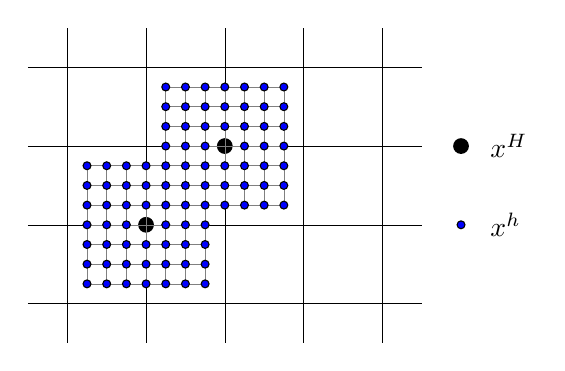
\begin{tikzpicture}
		%\draw[step = 0.25, dashed, color = gray ] (-0.5,-0.5) grid (4.5,3.5);
		\draw[step = 1, help lines, black] (0,0) grid (4,3);
		\fill (1,1) circle (.1);
		\fill (2,2) circle (.1);
		\draw[step = 0.25, help lines, gray] (0.25,0.25) grid (1.75,1.75);
		\draw[step = 0.25, help lines, gray] (1.25,1.75) grid (2.75,2.75);
		\draw[step = 0.25, help lines, gray] (1.75,1.25) grid (2.75,1.75);
		\draw[ help lines, gray] (1.75,1.25) -- (2.75,1.25) (1.25,1.75)--(1.25,2.75) ;
		\draw[ help lines, black] (-0.5,0) -- (0,0) (0,-0.5)--(0,0)(-0.5,1) -- (0,1) (-0.5,2) -- (0,2)(-0.5,3) -- (0,3)(1,-0.5)--(1,0)(2,-0.5)--(2,0)(3,-0.5)--(3,0)(4,-0.5)--(4,0)(0,3)--(0,3.5)(1,3)--(1,3.5)(2,3)--(2,3.5) (3,3)--(3,3.5)(4,3)--(4,3.5)(4,0)--(4.5,0)(4,1)--(4.5,1) (4,2)--(4.5,2) (4,3)--(4.5,3) ;
		\draw[fill = blue] (0.25,0.25) circle (.05)(0.25,0.5) circle (.05)(0.25,0.75) circle (.05)(0.25,1) circle (.05)(0.25,1.25) circle (.05)(0.25,1.5) circle (.05)(0.25,1.75) circle (.05)(0.5,0.25) circle (.05)(0.5,0.5) circle (.05)(0.5,0.75) circle (.05)(0.5,1) circle (.05)(0.5,1.25) circle (.05)(0.5,1.5) circle (.05)(0.5,1.75) circle (.05)(0.75,0.25) circle (.05)(0.75,0.5) circle (.05)(0.75,0.75) circle (.05)(0.75,1) circle (.05)(0.75,1.25) circle (.05)(0.75,1.5) circle (.05)(0.75,1.75) circle (.05)(1,0.25) circle (.05)(1,0.5) circle (.05)(1,0.75) circle (.05)(1,1.25) circle (.05)(1,.5) circle (.05)(1,1.75) circle (.05)(1,1.5) circle (.05)(1.25,0.25) circle (.05)(1.25,0.5) circle (.05)(1.25,0.75) circle (.05)(1.25,1) circle (.05)(1.25,1.25) circle (.05)(1.25,1.5) circle (.05)(1.25,1.75) circle (.05)(1.25,2) circle (.05)(1.25,2.25) circle (.05)(1.25,2.5) circle (.05)(1.25,2.75) circle (.05)(1.5,0.25) circle (.05)(1.5,0.5) circle (.05)(1.5,0.75) circle (.05)(1.5,1) circle (.05)(1.5,1.25) circle (.05)(1.5,1.5) circle (.05)(1.5,1.75) circle (.05)(1.5,2) circle (.05)(1.5,2.25) circle (.05)(1.5,2.5) circle (.05)(1.5,2.75) circle (.05)(1.75,0.25) circle (.05)(1.75,0.5) circle (.05)(1.75,0.75) circle (.05)(1.75,1) circle (.05)(1.75,1.25) circle (.05)(1.75,1.5) circle (.05)(1.75,1.75) circle (.05)(1.75,2) circle (.05)(1.75,2.25) circle (.05)(1.75,2.5) circle (.05)(1.75,2.75) circle (.05)(2,1.25) circle (.05)(2,1.5) circle (.05)(2,1.75) circle (.05)(2,2.25) circle (.05)(2,2.5) circle (.05)(2,2.75) circle (.05)(2.25,1.25) circle (.05)(2.25,1.5) circle (.05)(2.25,1.75) circle (.05)(2.25,2) circle (.05)(2.25,2.25) circle (.05)(2.25,2.5) circle (.05)(2.25,2.75) circle (.05)(2.5,1.25) circle (.05)(2.5,1.5) circle (.05)(2.5,1.75) circle (.05)(2.5,2) circle (.05)(2.5,2.25) circle (.05)(2.5,2.5) circle (.05)(2.5,2.75) circle (.05)(2.75,1.25) circle (.05)(2.75,1.5) circle (.05)(2.75,1.75) circle (.05)(2.75,2) circle (.05)(2.75,2.25) circle (.05)(2.75,2.5) circle (.05)(2.75,2.75) circle (.05);
		
		\fill (5,2) circle (.1);
		\node at (5.25,2)[right] {$x^{H}$};
		\draw[fill = blue] (5,1) circle (.05);
		\node at (5.25,1)[right] {$x^{h}$};
	\end{tikzpicture}
	\caption{Constructing the fine neighborhood $G^{h}_{\eta}$ given two active nodes $x^{H}$ in the coarse grid.}
\end{figure}
\begin{remark} 
As we shall see in \Cref{sec-conv}, we may need to consider mesh steps $H$ and $h$ with $h$ close to $H$, in particular such that $h > \frac{1}{2} H$.
In this case, the bound in  \eqref{constructfine} is equal to $h$.
In general, this bound is more efficient numerically, although any bound
in $[H/2,H]$ would work theoretically. 
\end{remark}

To solve the original minimum time problem, the computation will only be done in the selected fine grid nodes, which means that a full fast marching algorithm \Cref{fmalgo} is applied in the restricted fine grid $G^{h}_{\eta} $,
with the update operator of one direction HJ equation (for instance with target set $\destset$). 
We will denote by $V^{h,2}\todest$ the approximation of the value function $v\todest$ generated by the above 2-level algorithm on $G^h_\eta$.

The complete algorithm is shown in \Cref{2LFM}.
\begin{algorithm}[hbtp]
	\caption{Two-Level Fast-Marching Method (2LFM)} 
	\hspace*{0.02in} \leftline{{\bf Input:} Two grids  $X^h$ and $X^H$ with mesh steps $h<H$ respectively. The parameter $\eta_{H}>0$. }\\
\hspace*{0.02in} \leftline{{\bf Input:} 
Two update operators $\mathcal{U}\todest$ and $\mathcal{U}\fromsource$
adapted to both directions HJ equations.} 
\hspace*{0.02in} \leftline{{\bf Input:} Target sets: $\sourceset,\destset$.}\\
\hspace*{0.02in} \leftline{{\bf Output:} The fine grid \Fine  and approximate value function $V\todest^{h,2}$ on \Fine.}
	\begin{algorithmic}[1]
\State Apply \Cref{fmalgo} with Input grid $X^H$, update operator $\mathcal{U}\todest$, \Start$=\destset\cap X^H$ and \End$=\sourceset\cap X^H$, and 
output $V\todest^{H}$ and $A^H\todest$.
\State Apply \Cref{fmalgo} with Input grid $X^H$, update operator $\mathcal{U}\fromsource$, \Start$=\sourceset\cap X^H$ and \End$=\destset\cap X^H$, and 
output $V\fromsource^{H}$ and $A^H\fromsource$. 
		\For{Every node $x^{H}$ in $A\fromsource^H \cap A\todest^H$  }
		\If {$\F_{V^H(x)} \leq \min_{x^H \in X^H} \F_{V^H}(x^H) + \etaH$ } 
		\State Set $x^{H}$ as \Active. 
		\EndIf
		\EndFor
		\State Set \Fine to emptyset.
		\For{Every node $x^{H}$ in the \Active set}
		\For{Every $x^{h} \in X^h$ satisfying $\|x^{h} - x^{H} \|_{\infty} \leq \max \{ H-h,h\} $}
		\If{$x^{h}$ does not exist in set \Fine}
		\State Add $x^{h}$ in the set \Fine. 
		\EndIf
		\EndFor 
		\EndFor
		\State Apply \Cref{fmalgo} with Input grid \Fine, update operator $\mathcal{U}\todest$, \Start$=\destset\cap \Fine$ and \End$=\sourceset\cap \Fine$, and 
output $V\todest^{h,2}$.  
	\end{algorithmic}	\label{2LFM}
\end{algorithm}

\subsubsection{Correctness of~\Cref{2LFM}}\label{section-correct2}
In order to show the correctness of~\Cref{2LFM}, we first show that the computation in the fine grid is equivalent to the approximation of the value
function of a new optimal control problem, with a restricted state space. 

Let us first extend the approximate value function $V\fromsource^{H}$ and $V\todest^{H}$ from the nodes of $ X^{H}$ to the whole domain $\Omegab$ by a linear interpolation, and denote them by $V\fromsource^{H.I}, V\todest^{H,I}$ respectively. 
Then, we construct the region $O_{\eta}^{H,I}$ as follows:
\begin{equation}\label{OHIcoarse} 
    O^{H,I}_{\eta} = \{ x \in (\Omega \setminus (\sourceset \cup \destset) ) \mid \F_{V^{H,I}}(x) < \min_{x^H \in X^H} \F_{V^H}(x^H) + \etaH   \} \enspace.
\end{equation} 
$O^{H,I}_{\eta}$ can be thought as a continuous version of the set of active nodes in coarse grid,  and it is similar to the domain $\Oeta$ defined in \eqref{eqo}  -- the notation ``$I$''  stands for ``interpolation''. Notice that one can also do a regularization of $\F_{V^{H,I}}$ and thus of $O^{H,I}_{\eta}$  as in~\eqref{F_regu} and~\eqref{Oeta_regu} respectively. Thus, in the following we shall do as if $\partial O^{H,I}_\eta\setminus(\sourceset\cup\destset)$ is of class $\Cc^1$. We then consider the continuous optimal control problem {\rm (\ref{dynmsys},\ref{disc-cost},\ref{value-disc})} with new state space  $\overline{O^{H,I}_\eta}$, and the following new set of controls which is adapted to the new state constraint:
\begin{equation}  
	\A_{\etaH,x} = \{\alpha \in \mathcal{A} \ | \ y_{\alpha}(x; s) \in  \overline{O_{\eta}^{H,I}}, \text{ for all } s\geq0 \ \} \enspace.
\end{equation} 
Denote by $v\todest^{\etaH}$ the value function of this new state constrained problem. By \Cref{th_soner}, it is the unique solution of the new state constrained HJ equation $SC(F,O_{\eta}^{H,I},(\partial O_{\eta}^{H,I}) \cap (\partial \destset ))$. In our two level fast marching algorithm, we indeed use the grid $G^h_\eta$ to discretize $ \overline{O_{\eta}^{H,I}}$, then $V\todest^{h,2}$ is an approximation of $v\todest^{\etaH}$. 
Then, if $\overline{O_{\eta}^{H,I}}$ is big enough to contain the true optimal trajectories, by the results of \Cref{sec-cotra},  $v\todest^{\etaH}$ coincides with $v\todest$ on the optimal trajectories. Then, $V\todest^{h,2}$ is an 
approximation of $v\todest$ on  optimal trajectories. 
In the following result, we denote by $V^h\todest$ 
the solution of the discretization of
the HJ equation $SC(F,\Omega,\partial \destset)$ (associated to
Problem \eqref{problem}) on the grid $X^h$, or equivalently the
unique fixed point of $\mathcal{U}\todest$ satisfying the boundary conditions
on $X^h$, that is the output of \Cref{fmalgo} with input grid $X^h$, update operator $\mathcal{U}\todest$, \Start$=\destset\cap X^h$ and \End$=X^h$.
\begin{theorem}[Correctness of the Two-Level Fast-Marching Method]\label{lemmaOH} $ $
	\begin{enumerate}
	\item\label{lemmaOH-i} Assume \eqref{error_coarse} holds with $\gamma \leq 1$, and denote $C_\gamma := C\fromsource+C\todest$ and $L_v := L_{v\fromsource}+L_{v\todest}$, where $L_{v\fromsource}$ and $L_{v\todest}$ are the Lipschitz constants of $v\fromsource$ and  $v\todest$, respectively.
Then, there exists a constant $C_\eta> 0$ depending on 
$C_\gamma $ and $L_v$, such that for every $\etaH \geq  C_\eta H^{\gamma}$, 
	$\overline{O_{\eta}^{H,I}}$ contains the set $\Gamma^{*}$ of geodesic points for the continuous problem {\rm (\ref{dynmsys},\ref{disc-cost},\ref{value-disc})}.
	\item \label{lemmaOH-ii} If $\etaH$ is as in \eqref{lemmaOH-i}, there exists $\delta < \etaH$ depending on $\etaH$ and $H$ such that, for every $x \in G^h_{\eta} \cap \Gamma^{\delta}$, $V^{h,2}\todest(x) = V^h\todest(x)$. Thus,  $V^{h,2}\todest(x)$ converges towards $v\todest(x)$ as $h \to 0$.
	\end{enumerate}
\end{theorem}

\begin{proof}
	As shown in \Cref{pro-tra} ,  in a geodesic point $x$, the value function satisfies $\F_v(x) = v^*=\mathop{\min}\limits_{y \in \Omega} \F_v(y)$. 
	Consider a point $x^{'} \in \overline{\Omega \setminus (\sourceset \cup \destset)}\setminus \overline{O^{H,I}_{\eta}}$, 
	we have:  
	\[ \| V\fromsource^{H,I}(x^{'}) - v\fromsource(x^{'}) \| \leq C\fromsource H^{\gamma} + L_{v\fromsource} H, \quad \|V\todest^{H,I}(x^{'}) - v\todest(x^{'}) \| \leq C\todest H^{\gamma} + L_{v\todest} H \ . \]
	 Using the constants $C_\gamma = C\fromsource+C\todest$, and $L_v = L_{v\fromsource}+L_{v\todest}$, we have the following inequality:
	$$
	\begin{aligned}
		\F_{v}(x^{'}) &\geq \F_{V^{H,I}}(x^{'}) - (C_\gamma H^{\gamma}+L_v H) \geq \min_{x^H \in X^H} \F_{V^H}(x^H) +\etaH - (C_\gamma H^{\gamma} + L_v H) \\
		& \geq \min_{x \in \Omega} \F_v(x) + \etaH - 2(C_\gamma H^{\gamma} + L_v H) \ .
	\end{aligned}
	$$
	Thus, if we take $\etaH > 2(C_\gamma H^{\gamma} + L_v H)$, we have $x^{'} \notin \Gamma^{*}$. Since $\gamma \leq 1$, we can take 
$\etaH > C_\eta H^{\gamma}$, with an appropriate constant $C_\eta$.
This shows that $\Gamma^{*}\subset  \overline{O^{H,I}_{\eta}}$, that is the result of Point \eqref{lemmaOH-i}.

 The result of \eqref{lemmaOH-ii} is then straightforward using \Cref{valuefunction}.
\end{proof}

\subsection{Multi-level Fast Marching Method}
The computation in two level coarse fine grid can be extended to the multi-level case. In a nutshell, we construct finer and finer grids, considering the fine grid
of the previous step as the coarse grid of the current step, and defining the next
fine grid by selecting the actives nodes of this coarse grid.

\subsubsection{Computation in Multi-level Grids} Consider a $N$-level family of grids with successive mesh steps: $H_{1} \geq H_{2} \geq \dots \geq H_{N-1} \geq H_{N} = h,$ denoted $X^{H_i}$, for $i=1,\ldots, N$. Given a family of real positive parameters $\{\eta_1, \eta_2, \dots ,\eta_{N-1} \}$, the computation works as follows:

\textbf{\textit{Level-$1$:}} In first level, the computations are the same as  in coarse grid of the two level method (\Cref{2lfm_coarse}), with mesh step $H$ equal to $H_1$ and active nodes selected using the parameter $\eta$ equal to $\eta_1$. At the end of level-$1$, we get a set of active nodes: 
$O^{H_1}_{\eta_1}$.

\textbf{\textit{Level-$l$ with $1<l<N$:}} In level-$l$, we already know the set of active nodes in level-$(l-1)$, denoted $O^{H_{l-1}}_{\eta_{l-1}}$. 
We first construct the "fine grid" set of level-$l$ as in \eqref{constructfine}, that is:
\begin{equation}
	G^{H_{l}}_{\eta_{l-1}} = \{ x^{H_{l}} \in X^{H_{l}} \ | \ \exists \ x^{H_{l-1}} \in O^{H_{l-1}}_{\eta_{l-1}} : \| x^{H_{l-1}} - x^{H_{l}} \|_\infty \leq \max (H_{l-1}-H_{l},H_{l})  \} \enspace. 
\end{equation}
Then, we perform the fast marching in both directions in the grid $G^{H_{l}}_{\eta_{l-1}}$. 
This leads to the approximations $V\fromsource^{H_{l},l} $,  $V\todest ^{H_{l},l} $
and $\F_{V^{H_l,l}}$ of $v\fromsource$,  $v\todest$ and
$\F_v$ on grid $G^{H_{l}}_{\eta_{l-1}}$. 
 We then select the active nodes in level-$l$, by using the parameter $\eta_l$, as follows:
\begin{equation}
	O^{H_{l}}_{\eta_{l}} = \{ x^{H_{l}} \in G^{H_{l}}_{\eta_{l-1}} \ | \ \F_{V^{H_l,l}} (x^{H_l}) \leq \min_{ x^{H_{l}} \in G^{H_{l}}_{\eta_{l-1}} } \F_{V^{H_l,l}} (x^{H_l}) + \eta_l \ \} \enspace. 
\end{equation} 

\textbf{\textit{Level-N:}} In the last level, we only construct the final fine grid:
\begin{equation}
	G^{h}_{\eta_{N-1}} = \{ x^{h} \in X^{h} \ | \ \exists \ x^{H_{N-1}} \in O^{H_{N-1}}_{\eta_{N-1}} : \| x^{h} - x^{H_{N-1}} \|_\infty \leq \max (H_{N-1}-h, h )  \} \enspace.
\end{equation} 
Then, we only do the fast marching search in one direction in the grid $G^h_{\eta_{N-1}}$ and obtain the approximation $V\todest ^{h,N} $ of $v\todest$
on grid $G^{h}_{\eta_{N-1}}$. 

This algorithm is detailed in \Cref{MLFM}, and some possible grids generated  by our algorithm are shown in 
the following \Cref{sketchmlfh}. 

\begin{figure}[H]
	\centering
	\subfigure[Level-0]{
		\includegraphics[width=0.185\textwidth]{coarse.png}}
	\subfigure[Active Nodes]{
		\includegraphics[width=0.19\textwidth]{first.png}}
	\subfigure[Fine grid]{
		\includegraphics[width=0.16\textwidth]{fine_grid.png}}
	%$\Longrightarrow$
	\subfigure[Level-1]{
		\includegraphics[width=0.2\textwidth]{algorithm.png}}
	\dots
	\subfigure[Level-2]{
		\includegraphics[width=0.16\textwidth]{method.png}}
	
	\caption{Sketch of MLFM.}
	\label{sketchmlfh}
\end{figure}

\begin{algorithm}[htbp]
	\caption{Multi-Level Fast-Marching Method (MLFM)} 
		\hspace*{0.02in} \leftline{{\bf Input:} The mesh steps, grids, and selection parameters: $H_{l},X^{H_l},\eta_{l}$, for $l \in \{1,2,\dots,N\}$. }\\
	\hspace*{0.02in} \leftline{{\bf Input:} 
		Update operators $\mathcal{U}\todest$ and $\mathcal{U}\fromsource$
		adapted to both directions HJ equations and levels.} 
\hspace*{0.02in} \leftline{{\bf Input:} Target sets: $\sourceset,\destset$.}\\
\hspace*{0.02in} \leftline{{\bf Output:} The final fine grid \Fine  and approximate value function $V\todest^{h,N}$ on \Fine.}
	\begin{algorithmic}[1]
		\State 	Set \Coarsegrid to $X^{H_1}$.
		\For {$l = 1 \text{ to } N-1$}
		\State Do the partial fast marching search in \Coarsegrid \ in both directions. 
		\State Select the \Active nodes from the \Accepted nodes using $\eta_{l}$.
		\State Select the \Fine nodes based on the \Active nodes, and mesh step $H_{l+1}$.
		\State Let \Fine in current level be the new \Coarsegrid.
	\EndFor
	\State Do the partial fast marching search in only one direction in \Fine.
	\end{algorithmic}	\label{MLFM}
\end{algorithm}

In \Cref{MLFM}, 
Line-3 of  \Cref{MLFM} corresponds to lines-1 and 2 in \Cref{2LFM}, 
line-4 of  \Cref{MLFM}  corresponds to lines-3 to 7 in \Cref{2LFM}, 
line-5  of  \Cref{MLFM} corresponds to line-8 to line-15 in \Cref{2LFM}.  
\subsubsection{Correctness of~\Cref{MLFM}} 
In each level-$l$ with $l<N$,  
we have the approximate value functions $V^{H_{l}}\fromsource$ and $V^{H_{l}}\todest$ of $v\fromsource$ and $v\todest$ on the grid of level $l$. 
Then, we can apply the same constructions as in \Cref{section-correct2}
for the coarse grid $X^H$. This leads to a continuous version
$O_{\eta_{l}}^{H_{l},I}$ of the set of active nodes in level-$l$.
We also have sets $\mathcal{A}_{\eta_{l},x}$ of controls adapted 
to the optimal control problems of the form
{\rm (\ref{dynmsys},\ref{disc-cost},\ref{value-disc})}
with state space equal to the set $O_{\eta_{l}}^{H_{l},I}$,
and the corresponding value function $v^{\eta_{l}}\todest$,
which, 
by \Cref{th_soner}, is the unique solution of the new state constrained HJ equation $SC(F,O_{\eta_{l}}^{H_{l},I}, (\partial O_{\eta_{l}}^{H_{l},I}) \cap (\partial \destset))$. 
We can also consider the HJ equations in the direction "from source",
$SC(F^*,O_{\eta_{l}}^{H_{l},I},  (\partial O_{\eta_{l}}^{H_{l},I}) \cap (\partial \sourceset))$, and the corresponding value functions. 

The proof in the two level case can be easily adapted to multi-level case by showing that \Cref{lemmaOH} holds for each level $l<N$ with $H=H_l$ and $h=H_{l+1}$,
and for both directions. This leads to the following result, which proof is
clear. 
\begin{theorem}[Correctness of the Multi-level Fast-Marching Method] \
\label{theo-corr-multi}
	\begin{enumerate}
		\item\label{proofmlfm_i} Assume \eqref{error_coarse} holds for all $H>0$, with $\gamma \leq 1$, then there exists a constant $C_\eta\geq 0$ such that, for every $l \in \{ 1,2,\dots,N-1 \}$, for every $\eta_l \geq C_\eta (H_l)^{\gamma}$, $\overline{O^{H_l,I}_{\eta_l}}$ contains the set $\Gamma^{*}$ of geodesic points for the continuous minimum time problem{\rm (\ref{dynmsys},\ref{disc-cost},\ref{value-disc})}. 
		\item\label{proofmlfm_ii} Taking $\eta_l$ as proposed in \eqref{proofmlfm_i}, then there exists $\delta < \eta_{{N-1}}$ such that, for every $x \in G^h_{\eta_{N-1}} \cap \Gamma^\delta$, $ V^{h,N}\todest (x) = V^h\todest(x)$. Thus, $ V^{h,N}\todest(x)$ converges towards $v\todest(x)$ as $h \to 0$.
		\end{enumerate}
	\end{theorem}




\subsection{The Data Structure} 
In this section, we describe a dedicated data structure, which will
allow us to store the successive neighborhoods, and implement
the algorithm, in an efficient way.


Recall that for the classical fast-marching method, the data are normally stored using two types of structures \cite{bokanowski2010data}:
a full d-dimensional table (or tensor), which contains all the values 
of the current approximate value function on the whole discretization grid (the values are updated at each step); 
a dynamical linked list, which contains the information on the narrow band nodes with the current approximate value function. 

To implement efficiently our algorithms, we need to store the
successive (constrained) grids $G^{H_l}_{\eta_{l-1}}$, for every $l\in \{2,\dots,N\}$, in an efficient way.
A $d$-dimensional full table would be too expensive for the storage, since the complexity would be in the order of $(\frac{1}{h})^{d}$, which is impossible to implement for a small mesh step $h$ in high dimension. Moreover, the aim of our algorithm is to reduce the number of nodes in order to reduce the computational complexity, but this gain would be lost if we used a full table storage. We propose here a different storage of the grids $G^{H_l}_{\eta_{l-1}}$, in order to get a storage complexity in the order of the cardinality of these grids.

To implement our algorithm, we need to perform three type of operations,
when constructing the fine grid $G^{H_l}_{\eta_{l-1}}$ from the
active nodes, that is the elements of $O^{H_{l-1}}_{\eta_{l-1}}$:
\begin{enumerate}[label={\rm \arabic *.}] 
	\item Check if one node $x^{H_l}$ already exists in the grid; 
	\item Add one node $x^{H_l}$ into the existing grid; 
	\item Check the neighborhood information of one node $x^{H_{l-1}}$ 
or $x^{H_l}$. 
\end{enumerate}

We need to fulfil two goals. On the one hand, we want to keep the computational complexity for the operations "search" (the above steps 1 and 3) and "insert" (the above step 2) to be as low as possible, ideally in $O(1)$ time, since 
we need to do these operations at least once for every node of a grid.
On the other hand, we want the memory used to store
the grid at depth $l$ not to exceed
the size of the neighborhood of the ``small'' set $O^{H_{l-1}}_{\eta_{l-1}}$, interpolated in the fine grid of step $H_l$, avoiding to store
nodes outside this neighborhood. 

We used a "hash-table", to efficiently implement our algorithm. 
Suppose we are in the $d$-dimensional case. For the level-$l$ grid we have approximately $M_{l}$ nodes to store. For each node $x^l \in G^{H_l}_{\eta_{l-1}}$, we store three types of data in the hash table:
\begin{enumerate}[label={\rm \arabic *.}]
	\item  A $d$-dimensional vector of "int" type, which corresponds to it's position in $\R^d$ or equivalently its corresponding indices in the full $d$-dimensional table. 
	\item A "double' type data, which corresponds to it's value function. 
	\item Two "boolean" type data, for the fast matching search and selection of the active nodes.
	\end{enumerate}  

We then use the position of a node, $x^l \in \R^d$, as the "key" for the hash table to compute the corresponding slot by a hash function $h(x^l)$.  If several nodes have the same slot, i.e., a "collision" occurs, we need to attach to this slot the above data for each of these nodes. So we attach to a slot a vector, the entries of which are the above data for each node associated to this slot, see \Cref{hash-table}. 
The simple hash function we used is as follows:
\begin{equation}\label{hash}
	h(x^l) = ( \sum_{k = 1}^{d} x^{l}_{k} M_i^{'}) \mod 2{\overline{M_l}} \enspace.
\end{equation}
where $M_i^{'},i\in \{1,2,\dots,d \}$ is a random integer in $[1,2\overline{M_l}]$, and $\overline{M_l}$ is the predicted number of nodes in level-$l$ (which will be detailed later).
In fact, the hash function intends to reduce the "collisions", and numerical experiments show that this function could handle most of the cases well. In some particular case, it can be optimized using other hashing methods, for example the multiplication method or the universal hashing method~\cite{cormen2009introduction}.

\begin{figure}[htbp]
	\includegraphics[width=0.7\textwidth]{hash.png}
	\caption{The hash table to store fine grid nodes.}
\label{hash-table}
\end{figure}

\section{Computational Complexity}\label{sec-conv}
In previous section, we already proved that our algorithm
computes an approximation of the value of Problem \eqref{problem}, 
and of the set of its geodesic points, with an error depending on the
mesh step of the finest grid.
In this section, we analyze the space complexity and the computational complexity of our algorithm, and characterize 
the optimal parameters to tune the algorithm. 
In this section, we always use the following assumption:
\begin{assumption}\label{asspf_2}
The domain $\Omegab$ is convex and 
	there exist constants $\lowerboundf,\upperboundf$ such that:	
	$$ 0<\lowerboundf\leq f(x,\alpha)\leq \upperboundf <\infty, \text{ for all } x\in \Omega \text{ and } \alpha \in \mathcal{A} \enspace. $$
\end{assumption}
We will also assume that \eqref{error_coarse} holds for some
$\gamma>0$ and for all mesh sizes $H>0$, so that 
the conclusions of \Cref{lemmaOH} and \Cref{theo-corr-multi} hold. 
Consider first the two-level case, and suppose we want to get a numerical approximation of the value of Problem \eqref{problem} with an error bounded by some given $\varepsilon>0$, and a minimal total complexity. 
Three parameters should be fixed before the computation: 
\begin{enumerate}
\item The mesh step of the fine grid $h$;
	\item The mesh step of the coarse grid $H$;
	\item The parameter $\etaH$ to select the active nodes in coarse grid.
\end{enumerate} 
The parameter $h$ need to be small enough so that $C\todest h^\gamma\leq \varepsilon$ (using  \eqref{error_coarse}).
The parameter $\etaH$ is used to ensure that the subdomain $O^{H,I}_{\eta}$ does contain the true optimal trajectories, so it should be large enough
as a function of $H$, see \Cref{lemmaOH}, but we also
want it to be as small as possible to reduce the complexity.
Using the optimal values of $h$ and $\etaH$, the total
complexity becomes a function of $H$, when $\varepsilon$ (or $h$) is fixed. 
Then, one need to choose the optimal value of the parameter $H$ regarding
 this total complexity. 

In order to be able to estimate the total complexity, we shall also use the following assumption on the neighborhood of optimal trajectories:
\begin{assumption}\label{distance_beta}
The set of geodesic points $\Gamma^*$ consists of a finite number of optimal paths between $\sourceset$ and $\destset$. Moreover, 
	for every $x\in \mathcal{O}_{\eta}$, there exists $x^*\in \Gamma^*$ such that :
	$$\|x - x^*\| \leq C_\beta \eta^\beta \ ,$$
	where $0<\beta \leq 1$, and $C_\beta$ is a positive constant.
	\end{assumption} 

Let us denote by $D$ the maximum Euclidean distance between the points in $\sourceset$ and $\destset$, i.e.\ $D = \sup \{ \|x-y \| \mid x\in \sourceset, y \in \destset  \}$, and by $D_\Omega$  the diameter of $\Omegab$, i.e.\ 
$D = \sup \{ \|x-y \| \mid x,y\in \Omegab  \}$.
For any positive functions $f,g:\R^p\to\R_{>0}$ of $p$ real parameters,
the notation $g(x)=\widetilde{O}(f(x))$ will mean
$g(x)=O(f(x)(\log(f(x)))^q)$ for some integer $q$,
that is $|g(x)|\leq C f(x)|\log(f(x))|^q$ for some constant $C>0$.
We have the folowing estimate of the space complexity.
\begin{proposition}\label{complexity-2level}
Assume that $H\leq D$, and that $\etaH$ satisfies the condition of \Cref{lemmaOH} and $\etaH\leq D$.
There exists a constant $C>0$  depending on $D_\Omega$, 
$D$, $\upperboundf$ and $\lowerboundf$, 
$\beta$, $\gamma$, $C_\beta$, $C_\gamma$ and $L_v$ (see \Cref{lemmaOH}),
such that
       the space complexity $\spacecom(H,h)$ of the two level fast marching algorithm with coarse grid mesh step $H$, fine grid mesh step $h$ and parameter $\eta_H$  is as follows:
	\begin{equation} \label{e-complexity}
		\spacecom(H,h) = \widetilde{O}\Big( C^d \Big( \frac{1}{H^d} + \frac{(\eta_H)^{\beta(d-1)}}{h^d} \Big)\Big) \enspace.
	\end{equation} 
\end{proposition} 
\begin{proof}
  Up to a multiplicative factor, in the order of $d$ (so which enters in the 
$\widetilde{O}$ part) the space complexity is equal to the total
  number of nodes of the coarse and fine grids.
  
  We first show that up to a multiplicative factor, the first term
  in~\eqref{e-complexity},  $(\frac{C}{H})^{d}$, is the number of accepted nodes in the coarse-grid.
  To do so, we exploit 
  the monotone property of the fast-marching update operator. Recall that in the coarse grid, we incorporate dynamically new nodes by partial fast-marching, starting from $\sourceset\cap X^H$ (resp. $\destset\cap X^H$) until $\destset\cap X^H$ (resp. $\sourceset\cap X^H$) is accepted. 
  
  Let us first consider the algorithm starting from $\sourceset$. In this step, let us denote $\dest^f$ the last accepted node in $\destset$, then we have for all the nodes $x^{H}\in A\fromsource^H$ that have been accepted, $V^H\fromsource(x^{H}) \leq V^H\fromsource(\dest^f)$. Then, using \eqref{error_coarse}), we obtain  $v\fromsource(x^{H}) \leq v\fromsource(\dest^f)+2 C\fromsource H^\gamma \leq v\fromsource(\dest^f)+2 C\fromsource D^\gamma$,
 which gives the following inclusion, when $D$  and $T\fromsource(\dest^f)$ are
small enough: 
  \begin{align*}
A\fromsource^H
&\subseteq \{ x\in \Omegab \mid v\fromsource(x) \leq v\fromsource(\dest^f) +2C\fromsource H^\gamma\} \\
&\subseteq \{ x\in \Omegab \mid T\fromsource(x) \leq T\fromsource(\dest^f) -\log(1-2C\fromsource D^\gamma e^{T\fromsource(\dest^f)}) \} \ . 
\end{align*}

Let $x\in \Omegab$,  recall that $T\fromsource(x)$ is the minimum time traveling from $x$ to $\sourceset$, then we have for some $\source^i \in \sourceset$,
  \begin{equation}\label{leftside}
  	\| x - \source^i \| \leq \int_{0}^{T\fromsource(x)} \|\dot{x}(t)\| dt \leq \upperboundf T\fromsource(x) \ .
  	\end{equation}
  Moreover, we have for some $\source^j \in \sourceset$,
  \begin{equation}\label{rightside}
  	T\fromsource(\dest^f) \leq \frac{\| \dest^f - \source^j \|}{\lowerboundf} \leq \frac{D}{\lowerboundf}\ ,
  	\end{equation}
  since we can take a control $\alpha$ proportional to $\dest^f - \source^j$, so that the trajectory given by \eqref{dynmsys_t} follows the straight line from $\source^j$ to $\dest^f$ (with variable speed). Combine \eqref{leftside} and \eqref{rightside}, we have for the set of accepted nodes:
 \begin{align*}
A\fromsource^H &\subseteq \{x \mid  \| x- \source^i\| \leq ({\upperboundf D}/{\lowerboundf})
-\upperboundf  \log(1-2C\fromsource D^\gamma e^{{\upperboundf D}/{\lowerboundf}})  , \;  \text{for some} \ \source^i \in \sourceset \} \ .
\end{align*}
  Thus, all the nodes we visit are included in a $d$-dimensional ball with radius $R$, where $R$ is a constant depending on $D$, ${\upperboundf}$, ${\lowerboundf}$, $C\fromsource$ and $\gamma$, when $D$ is small enough.
Otherwise, since $\Omegab$ has a diameter equal to $D_\Omega$, one can take $R=D_\Omega$.
Then, the total number of nodes that are accepted in the coarse grid  is bounded by $(\frac{C}{H})^{d}$, in which $C/R$ is a positive constant in the order of 
$(\upsilon_d)^{1/d}$, where $\upsilon_d$ is the volume of unit ball in $\R^d$,
and satisfying $C/R\leq 2$, so we can take $C/R=2$. % factor  
  The same result can be obtained for the search starting from $\destset$.

  We now show that, still up to a multiplicative factor,
  the second term in~\eqref{e-complexity},
  $D\frac{(\eta_H)^{\beta(d-1)}}{h^d}$, is the number of nodes of the fine-grid. 
  Consider a node $x^{h} \in G^{h}_{\eta}$. By definition, there exists $x^H\in O^H_\eta$ such that $\|x^h-x^H\|\leq H$. 
	 Denote $C_\gamma = C\fromsource+C\todest$, and $L_v = L_{v\fromsource}+L_{v\todest}$ (the sum of the Lipschitz constants of $v\todest$ and $v\fromsource$).
Then, using similar arguments as in the proof of \Cref{lemmaOH}, we obtain:
\begin{align*}
\F_{v}(x^h) &\leq \F_v(x^H)+L_v \|x^h-x^H\| \\
& \leq \F_{V^H}(x^H)+C_\gamma H^\gamma+ L_v H\\
&\leq  \min_{y^H\in X^H} \F_v(y^H)+\eta_H+ C_\gamma H^\gamma+L_v H\\
&\leq  \min_{y\in \Omega } \F_v(y)+\eta_H+ C_\gamma H^\gamma+2 L_v H\enspace .
\end{align*}

This entails that $x^h \in \mathcal{O}_{\eta_H + \epsH }$,
with $\epsH=C_\gamma H^\gamma+2 L_v H$. 
Since $\gamma \leq 1$, so $\epsH$ is of order $H^\gamma$, 
and $\etaH\geq C_\eta H^\gamma$ by assumption,
then using \Cref{distance_beta}, 
we deduce that for some positive constant $C'$, depending on 
$\beta,\; \gamma$, $C_\beta$, $C_\gamma$, and $L_v$, 
 there exists $x^*\in \Gamma^*$
such that 
\begin{equation}\label{nodedistance}
	\|x^{h}-x^* \| \leq C' (\etaH)^\beta \enspace.
\end{equation}
	
We assume now that $\Gamma^*$ consists of a single optimal path 
from $\source\in\sourceset$ to $\dest\in\destset$.
Indeed, the proof for the case of a finite number of paths is similar
and leads to a constant factor in the complexity, which 
is equal to the number of paths.
Up to a change of variables, we get a parametrization of $\Gamma^*$ as the image of a one-to-one map $\phi: t\in [0,D_{\Gamma}]\mapsto \phi(t)\in \Gamma^*$, 
with unit  speed $\|\phi'(t)\|=1$, where $D_\Gamma$ is a positive constant.
Let us denote in the following by $d_{\Gamma^*}(x,y)$ the distance between two points $x,y \in \Gamma^*$ along this path,
that is $d_{\Gamma^*}(x,y)=|t-s|$ if $x=\phi(t)$ and $y=\phi(s)$, with $t,s\in  [0,D_{\Gamma}]$. Since the speed of $\phi$ is one,
we have $\|x-y\|\leq d_{\Gamma^*}(x,y)$, and so $D\leq D_\Gamma$.
Moreover, by the same arguments as 
above, we have $D_\Gamma\leq \upperboundf D/\lowerboundf$.

Let us divide  $\Gamma^*$, taking equidistant points $x_0, x_1,x_2,...,x_N,x_{N+1} \in \Gamma^*$ between $x_0=\source$ and $x_{N+1}= \dest$, with $N = \lfloor 
D_\Gamma 
 /( C'(\eta_H)^\beta )\rfloor$, so that 
$d_{\Gamma^*}(x_{k},x_{k+1}) = D_\Gamma/ (N+1) \leq C' (\eta_H)^\beta\; \forall k \in \{ 0, 1,2,...,N \}$. 
Set $\Gamma^*_{\mathrm{dis}}:= \{ \source, x_1,x_2,...,x_N, \dest \}$.
Then, by \eqref{nodedistance}, we have for every $x^h \in G^h_\eta$, there exists a point $x \in \Gamma^*_{\mathrm{dis}}$ such that :
$$ \|x^h - x  \| \leq \frac{3}{2} C' (\eta_H)^\beta \ .$$
Let us denote $B^d(x,r)$ the $d$-dimensional open ball with center $x$ and radius $r$ (for the Euclidian norm).
Taking, $\Delta := \frac{3}{2}C' (\etaH)^\beta  + \frac{h}{2}$, we deduce:
$$ \bigcup_{x \in G^h_\eta}B^d(x,\frac{h}{2}) \subset \bigcup_{x\in \Gamma^*_{\mathrm{dis}}} B^d(x,\Delta)  \ .$$ 
Moreover, since the mesh step of $G^h_\eta$ is $h$, all balls centered in $x\in G^h_\eta$ with radius $\frac{h}{2}$ are disjoint, which entails:
$$\operatorname{Vol} \Big(\bigcup_{x \in O^h_\eta}B^d(x,\frac{h}{2})\Big) = |G^h_\eta| (\frac{h}{2})^d \upsilon_d \ , $$ 
where $\upsilon_d$ denotes the volume of the unit ball in dimension $d$, and $|G^h_\eta|$ denotes the cardinality of $G^h_\eta$, which is also the number of nodes in the fine grid. Thus, we have:
$$
|G^h_\eta| = \frac{\operatorname{Vol} \Big(\bigcup_{x \in O^h_\eta}B^d(x,\frac{h}{2})\Big)}{(\frac{h}{2})^d \upsilon_d} \leq \frac{\operatorname{Vol}\Big( \bigcup_{x\in \Gamma^*_{\mathrm{dis}}} B^d(x,\Delta) \Big)}{ (\frac{h}{2})^d \upsilon_d} \leq |\Gamma^*_{\mathrm{dis}}| 2^d \frac{\Delta^d}{h^d} \enspace .
$$
Since $\etaH\geq C_\eta H^\gamma$, $h\leq H$ and $\beta,\gamma\leq 1$, we get that  
$\Delta\leq C'' (\etaH)^\beta$ for some constant $C''$ depending on $C_\eta$, 
$C'$, $\beta$ and $\gamma$.
Then, 
\[ |G^h_\eta|  \leq D' \frac{(2C''(\etaH)^{\beta})^{d-1} }{h^d} \ ,\]
where $D'$ depends on $D_\Gamma$, $D$ and $C'$.
This leads to the bound of the proposition. 
\end{proof} 

 \begin{remark}
For the fast marching method with semi-lagrangian scheme, the computational complexity $\computcom$  satisfies  $\computcom=\widetilde{O}(3^d \spacecom)$.
Then, the same holds for the two-level or multi-level fast marching 
methods. 
In particular for the  two-level fast marching method
$\computcom$ has same estimation as $\spacecom$ in \Cref{complexity-2level}.
 	\end{remark}

The same analysis as in two level case also works for the $N-$level case, for which we have the following result:
\begin{proposition}\label{prop-multi-complexity}
Assume that $H_1\leq D$, and that, 
for $l=1,\ldots, N-1$, $\eta_l$ satisfies the condition of \Cref{theo-corr-multi}, and $\eta_l\leq D$.
Then, 	the total computational complexity $\computcom (H_{1},H_{2},\dots,H_{N})$ of the multi-level fast marching algorithm with $N$-levels, with grid mesh steps $H_{1} \geq H_{2} \geq ,\dots, \geq H_{N-1} \geq H_{N} = h$ is 
	\begin{equation}\label{com_ml}
		\computcom (\{H_l\}_{1 \leq l \leq N}) = \widetilde{O}\Big( C^d \Big( \frac{1}{(H_{1})^d} + \frac{(\eta_1)^{\beta(d-1)}}{(H_2)^d}+ \frac{(\eta_2)^{\beta(d-1)}}{(H_3)^d}+ \dots+ \frac{(\eta_{N-1})^{\beta(d-1)}}{h^d}\Big)\Big)\enspace ,
	\end{equation}
with $C$ as in \Cref{complexity-2level}.
Moreover, the space complexity has a similar formula.\hfill \qed
\end{proposition}

Minimizing the formula in \Cref{complexity-2level}
 and \Cref{prop-multi-complexity}, 
we obtain the following result of the computational complexity.

\begin{theorem}\label{complexity_1}
Assume $d\geq 2$, and let $\nu:=\gamma\beta (1-\frac{1}{d})<1$.
Let $\varepsilon>0$, and choose $h = (C_\gamma^{-1} \varepsilon)^{\frac{1}{\gamma}}$.
Then, there exist some constant $C_m$ depending on the same parameters as 
in \Cref{complexity-2level}, such that,
in order to obtain an error bound on the value of Problem \eqref{problem} 
less or equal to $\varepsilon$ small enough,
one can use one of the following methods:
	\begin{enumerate}
		\item\label{complexity_i} The two-level  fast marching method with $ \eta_H =C_\eta H^ \gamma$, and 
$H = h^{\frac{1}{\nu+1}}$.
In this case, the total computational complexity is $\computcom(H,h) = \widetilde{O}((C_m)^d (\frac{1}{\varepsilon})^{\frac{d}{ \gamma (\nu+1)}} )$.  
		\item\label{complexity_ii}
The $N-$level fast marching method
with $\eta_l = C_\eta H^\gamma_l$ and $H_l = h^{ \frac{1 - \nu^l }{ 1 - \nu^N } }$, for $l=1,\dots,N-1$. In this case,  the total computational complexity is  $\widetilde{O}(N (C_m)^d (\frac{1}{\varepsilon})^{ \frac{1 - \nu}{ 1 - \nu^N }\frac{d}{\gamma} }  )$. 
		\item\label{complexity_iii} The $N-$level fast marching method 
with  $N=\lfloor \frac{d}{\gamma}  \log(\frac{1}{\varepsilon}) \rfloor$, 
and  $\eta_l = C_\eta H_l^\gamma$ and $H_l =h^{\frac{l}{N}}$,
for $l=1,\dots,N-1$. 
 Then, the total computational complexity reduces to $\widetilde{O}((C_m)^d (\frac{1}{\varepsilon})^{(1-\nu)\frac{d}{\gamma}})=\widetilde{O}((C_m)^d (\frac{1}{\varepsilon})^{\frac{1+(d-1)(1-\gamma \beta)}{\gamma}})$.
When $\gamma=\beta=1$, it reduces to $\widetilde{O}((C_m)^d \frac{1}{\varepsilon})$.
		\end{enumerate}
	\end{theorem}
\begin{proof} 
  For~\eqref{complexity_i}, 
using \eqref{error_coarse} together with \Cref{lemmaOH},
which applies since $ \eta_H = C_\eta H^ \gamma$,
 we get that the error on the value obtained by the
 two-level  fast marching method 
is less or equal to $C_\gamma h^\gamma=\varepsilon$. 
Note that in order to apply 
\Cref{lemmaOH}, 
$\eta_H$ needs to satisfy $ \eta_H \geq C_\eta H^ \gamma$. 
Then, to get a minimal computational complexity, one need
to take $ \eta_H =C_\eta H^ \gamma$ as in the theorem.
We obtain the following total computational complexity: 
  \begin{equation}\label{com_2l_1}
	\computcom (H,h) = \widetilde{O}( (C')^{d} (H^{-d} + {h^{-d}} H^{ \gamma \beta(d-1)} ))\enspace,
\end{equation}
for some new constant $C'=C\max(1, C_\eta)^{\beta}$.
When $h$ is fixed, this is a function of $H$ which gets its minimum value for
\begin{equation}\label{minim_H_1}
	H = 
C_1  h^{\frac{d}{(\gamma \beta+1)d-\gamma \beta}} \quad \text{with}\quad C_1=\big(\frac{d}{ \gamma \beta(d-1)}\big)^{\frac{1}{(\gamma \beta + 1)d- \gamma \beta}}\enspace,
	\end{equation}
since it is decreasing before this point and then increasing. 
Then, the minimal computational complexity bound is obtained by 
substituting the value of  $H$ of \eqref{minim_H_1} in \eqref{com_2l_1}.
The formula of $H$ in \eqref{minim_H_1}  is as in~\eqref{complexity_i}, up to the multiplicative factor $C_1>0$. One can show that $1\leq C_1\leq C_2$ with $C_2$ depending only on $\gamma\beta$.
Hence, substituing this value of $H$ instead of the one of \eqref{minim_H_1}
in  \eqref{com_2l_1},
gives the same bound up to the multiplicative factor $C_1^d$.
So in both cases, using
$h = (C_\gamma^{-1} \varepsilon)^{\frac{1}{\gamma}}$,
we obtain a computational complexity bound as in~\eqref{complexity_i},
for some constant $C_m$ depending on the same parameters as 
in \Cref{complexity-2level}. 
  
  For~\eqref{complexity_ii}, 
using this time \eqref{error_coarse} together with \Cref{theo-corr-multi}, 
and that $\eta_l = C_l H_l^{\gamma}$, we get that the error on the value obtained by the multi-level fast marching method 
is less or equal to $C_\gamma h^\gamma=\varepsilon$.
As in~\eqref{complexity_i}, we 
apply the formula of \Cref{prop-multi-complexity}
 with $\eta_l = C_l H_l^{\gamma}$, which gives 
  \begin{equation}\label{com_ml_2}
  \computcom(\{H_l\}_{1\leq l \leq N}) = \widetilde{O}\Big((C')^d ((H_1)^{-d}  +(H_1)^{\gamma \beta(d-1)} (H_2)^{-d} + \dots + (H_{N-1})^{ \gamma \beta(d-1)} h^{-d}  \Big) \  ,
  \end{equation}
for the same constant $C'$ as above.
This is again a function of $H_1, H_2,\dots,H_{N-1}$ when $h$ is fixed. We deduce the optimal mesh steps $\{ H_1, H_2,\dots,H_{N-1} \}$ by taking the minimum of $\computcom(\{H_l\}_{1\leq l \leq N})$ with respect to $H_1, H_2,\dots,H_{N-1}$,
and then simplifying the formula by eliminating the constants. 
We can indeed proceed by induction on $N$, and use iterative formula 
similar to \eqref{minim_H_1}. 
We then obtain the formula for $H_l$ as in~\eqref{complexity_ii}.  Substituting these values of the $H_l$ into \eqref{com_ml_2}, 
for a general $d\geq 2$, we obtain the following bound on the 
total computational complexity 
\begin{equation}\label{comp-N}
	\computcom(\{H_l\}_{1\leq l \leq N}) =\widetilde{O}(N (C')^d (\frac{1}{h})^{ \frac{1-\nu}{1-\nu^N} d})
	\enspace .\end{equation}
Now using $h = (C_\gamma^{-1} \varepsilon)^{\frac{1}{\gamma}}$, we get the
formula of~\eqref{complexity_ii}. 
  
For \eqref{complexity_iii}, 
let us  first do as if $\nu =1$.
 In that case, passing to the limit when $\nu$ goes
to $1$ in previous formula, we obtain the new formula for the $H_l$ given in
 \eqref{complexity_iii}.
We also obtain a new formula for the total complexity in \eqref{comp-N}
of the form $\widetilde{O}(N (C')^d (\frac{1}{h})^{ \frac{d}{N}})$.
The minimum of this formula with respect to $N$ is obtained for
$N = d\log(\frac{1}{h})$ which with
 $h = (C_\gamma^{-1} \varepsilon)^{\frac{1}{\gamma}}$, 
leads to a formula of $N$ in the order of  the one of~\eqref{complexity_iii}.
Let us now substitute the values of $H_l$ into the complexity formula~\eqref{com_ml_2}, we obtain the total computational complexity (for $h$ small enough)
\begin{equation}\label{com_ml_3}
	\computcom(\{H_l\}_{1\leq l \leq N}) = \widetilde{O}\Big( (C')^d (\frac{1}{h})^{\frac{d}{N}} \sum_{l=0}^{N-1} (\frac{1}{h})^{\frac{l}{N}(1-\nu)d} \Big) = \widetilde{O}\Big( N(C')^d (\frac{1}{h})^{\frac{d}{N}} (\frac{1}{h})^{(1-\nu)d} \Big) \ . 
\end{equation}
Now taking $N = \lfloor \frac{d}{\gamma}  \log(\frac{1}{\varepsilon}) \rfloor$ and using again $h = (C_\gamma^{-1} \varepsilon)^{\frac{1}{\gamma}}$, we get the
formula of~\eqref{complexity_iii}.
\end{proof}

\begin{remark}\label{rem-implem}
  In Point~\eqref{complexity_iii} of \Cref{complexity_1},
  we can replace $N$ by any formula of the form $N=\lfloor \kappa d \log(\frac{1}{h}) \rfloor$,  with a constant  $\kappa>0$.
  In that case, the number of levels and the parameters $H_l$
  (the intermediate mesh steps) only depend on the final mesh step $h$ and the
  dimension.
  However, the conditions on the parameters $\eta_l$ depend on the parameters
  $\gamma$ and $C_\eta$ of the problem to be solved and thus are difficult to
  estimate in practice. Moreover, it may happen that the upper bound
  $C_\eta$ is too large, making the theoretical complexity too large in
  practice even when $\gamma\beta=1$.
\end{remark}

\begin{remark}
	In~\Cref{complexity_1}, the theoretical complexity bound highly depends on the value of $\gamma \beta$. For the first constant $\gamma$, which is the convergence rate of the fast marching method, the usual finite differences or semilagrangian schemes satisfy $\gamma = \frac{1}{2}$. However, it may be equal to $1$, which typically occurs under a semiconcavity assumption (see for instance~\cite{camilli1996approximation,falcone2013semi}). Higher order schemes (in time step) may also be used, under some additional regularity on the value function, see for instance~\cite{falcone1998convergence,bokanowski2015value} and lead to $\gamma\geq 1$.

Recall that the second constant $\beta$,  defined in \Cref{distance_beta}, 
determines the growth of the neighborhood $\mathcal{O}_{\eta}$ of the optimal trajectories, as a function of $\eta$. 
    This exponent depends on the geometry of the level sets of the value function. We provide some examples for which $\beta=1$ in \Cref{appen_beta}. 
In particular, one can find examples such that $\gamma=\beta=1$.
	\end{remark}
	


\section{Numerical Experiments}\label{sec-test}

In this section, we present numerical tests, showing the improvement of our algorithm,  compared with the original fast-marching method of Sethian et al.~\cite{sethian1996fast,sethian2001ordered}, using the same update operator.
Both algorithms were implemented in C++, and executed on a single core of a Quad Core IntelCore I7 at 2.3Gh with 16Gb of RAM.

Note that, as said in \Cref{rem-implem}, the constant $C_\eta$ in
the formula of the parameters $\eta_l$ of the multi-level fast marching
method is difficult to estimate. Then,
for a given problem, first several tests of the algorithm are
done for large values of the mesh steps (or on the first levels of
the multi-level method) with some initial guess of the constant
$C_\eta$, assuming that $\gamma=1$. This is not too expensive,
so we do not count it in the total CPU time of the multi-level fast marching
method. 

\subsection{The tested problems} In the numerical tests,  we shall consider the following particular problems in several dimensions $d$.

\begin{test}[Euclidean distance in a box]\label{Case1} 
We start with the easiest case: a constant speed $f(x,\alpha) \equiv 1$ in $\Omega = (0,1)^{d}$. The sets $\sourceset$ and $\destset$ are the Euclidean balls with radius $0.1$, centered at $(0.2,\dots,0.2)$ and $(0.8,\dots,0.8)$ respectively. 
\end{test}

\begin{test} 
[Discontinuous speed field] \label{Case2}
The domain $\Omega$ and the sets $\sourceset$, $\destset$ are the same as in \Cref{Case1}. 
The speed function is discontinuous, with the form: 
$$
f(x,\alpha) = 
\left\{ 
\begin{aligned}
	& 0.3, \quad &x \in (0.4,0.6)^{d},\\
	& 1,  &\text{elsewhere}.
\end{aligned}
\right.
$$ 
Thus, the speed is reduced in a box centered in the domain. In this case, optimal trajectories must ``avoid'' the box, so there
are $2{d \choose 2} = d(d-1)$ optimal trajectories from $\sourceset$ and $\destset$, which are obtained by symmetry arguments.
\end{test}
\begin{test}[The Poincar\'e Model] 
\label{Case3}
Consider the minimum time problem in the open unit Euclidian ball $\Omega = B^d(0,1)$. The sets $\sourceset$ and $\destset$ are the Euclidean balls with radius $\frac{0.1}{\sqrt{d}}$, centered at $ (\frac{-0.8}{\sqrt{d}},\dots,\frac{-0.8}{\sqrt{d}})$ and $(\frac{0.8}{\sqrt{d}},\dots,\frac{0.8}{\sqrt{d}})$ respectively. This speed function $f$ is given as follows:
\[   f(x,\alpha) = 1 - \|x\|^2 \ . \] 
This particular choice of vector field corresponds to the Poincar\'e model of the hyperbolic geometry, that is, the optimal trajectories of our minimum time problem between two points are geodesics or ``straight lines'' in the hyperbolic sense. 
\end{test} 

\begin{test}\label{Example 1.a} 
Consider $\Omega = B^d(0,1)$, the open unit Euclidian ball, and 
let $\sourceset$ and $\destset$ be the closed balls with radius $r/2$ and
centers $(1-r,0,\dots,0)$ and $(-1+r,0,\dots,0)$, respectively,
with $0<r < \frac{1}{2}$. 
 For every $x=(x_1,x_2,\dots,x_d)\in\Omega$ and $\alpha \in \A$, the speed is given as follows:
\begin{equation}\label{dynamic_ex1}
	f(x,\alpha) = 1+x_1^2-\sum_{i=2}^d x_i^2 \ .
\end{equation} 
We prove in~\Cref{appen_beta-1} of \Cref{appen_beta} that this problem satisfies $\beta=1$.
\end{test}

\begin{test} \label{Example 1.b}  
We address the problem with same domain and speed as in \Cref{Example 1.a}, but
with the same source and destination sets as in \Cref{Case3}. 
\end{test}


\subsection{Comparison between ordinary and multi-level fast-marching methods} 
We next provide detailed results comparing the performances of
the classical and multi-level fast marching methods in the special case
of~\Cref{Case1}.
Detailed results concerning Problems~\ref{Case2}--\ref{Example 1.b}
are given in \Cref{num_data}, showing a similar gain in performance. 
In the higher dimension cases, the classical fast marching method 
cannot be executed in a reasonable time. So we fix a time budget of 1 hour,
that is we show the results of these algorithms when they finish 
in less than 1 hour only.
\Cref{test1_1} shows the CPU time and the memory allocation for~\Cref{Case1} in dimensions range from 2 to 6, with grid meshes equal to $\frac{1}{50}$ and $\frac{1}{100}$.
In all the dimensions in which both methods can be executed in less
than one hour, 
 we observe that the multi-level fast marching method with finest mesh step $h$ yields the same relative error as the classical fast marching method with mesh step $h$, but with considerably reduced CPU times and memory requirements. 
 Moreover, when the dimension is greater than 4, the classical fast marching method could not be executed in a time budget of 1 hour.
In all, the multi-level method appears to be much less sensitive to the \textit{curse-of-dimensionality}. 

\begin{figure}[htbp]
	\centering 
		\includegraphics[width=0.45\textwidth]{CPU_dimension_1.png} 
		\includegraphics[width=0.45\textwidth]{memory_dimension_1.png}
	\caption{ \Cref{Case1}. CPU time (left) and memory allocation (right) as a function of the dimension, for a fixed finest mesh step $h$.}
	\label{test1_1}
\end{figure}

To better compare the multi-level method with the classical method, we test the algorithms with several (finest) mesh steps (which are proportional to the predictable error up to some exponent $1/\gamma$), when the dimension is fixed to be $3$, see~\Cref{test1error}. We consider both the 2-level algorithm and the multi-level algorithm. In the multi-level case, the number of levels is adjusted to be (almost) optimal for different mesh steps and dimensions. 

\begin{figure}[htbp]
	\centering
\subfigure[CPU time as a function of $\frac{1}{h}$]{
	\label{t1_h}
	\includegraphics[width=0.45\textwidth]{cpu_mesh_1.png}}
	\subfigure[Memory allocation as a function of $\frac{1}{h}$]{
	\label{t1_logh}
	\includegraphics[width=0.45\textwidth]{memory_mesh_1.png}}
\caption{\Cref{Case1}. CPU time and memory allocation 
for several values of the finest mesh step $h$, in dimension $3$.}
\label{test1error}
\end{figure} 

\subsection{Effective complexity of the multi-level fast-marching method}
We next analyse the experimental complexity of the multi-level fast marching method in the light of the theoretical estimates of \Cref{complexity_1}.
For this purpose, we tested the multi-level fastmarching method on
Problems~\ref{Case1}--\ref{Example 1.b}, with an almost optimal number
of levels, and several dimensions and final mesh steps.
For all these cases, we compute the (logarithm of) CPU time
and shall plot it as a function of the dimension, or of
the final mesh step.

If the number of levels is choosen optimal as in \Cref{complexity_1},
we can expect a complexity 
in the order of 
$\widetilde{O}(C^d (\frac{1}{\varepsilon})^{\frac{1+(d-1)(1-\gamma \beta)}{\gamma}})$,
depending on the model characteristics, to be compared with $(\frac{1}{\varepsilon})^{\frac{d}{\gamma}}$ for the usual
fast marching method.
This means that the logarithm of CPU time should be of the form
\begin{equation}\label{theoretical-estimation}
  \log (\text{CPU time})\simeq 
  s_0+ s_2  \log (\frac{1}{h})+ (s_1+s_3 \log (\frac{1}{h})) d =s_0+s_1d +(s_2+s_3 d) \log (\frac{1}{h}) 
  \enspace,\end{equation}
where $s_1=\log(C)$, $s_2= \gamma \beta\in (0,1]$ and $s_3=1-\gamma\beta$. 
To check if such an estimation of complexity holds, we shall
execute the multi-level fastmarching method on
all the problems for several values of $h$ and $d$, and 
compute the logarithm of the CPU time
as a function of the dimension and then as a function of $\log(1/h)$.
However, choosing an optimal number of levels may be difficult to implement due
to the small differences between the mesh steps.
So, the results will not always fit with the above theoretical prediction.

We first present tests done for dimension $2$ to $6$ and finest mesh step $\frac{1}{50}$ and $\frac{1}{100}$, for which we compute the (logarithm of) CPU time.
We show in \Cref{summaryfig_1}, the graph of the logarithm of CPU time
as a function of the dimension (when finest mesh step is fixed), 
for which the form~\eqref{theoretical-estimation} suggests a slope of the form $s_1 + s_3 \log(\frac{1}{h})$.
We also give the precise values of these functions
in \Cref{summary_1}, where we compute the slope by linear regression. 
If the slope satisfies this formula, then one can get an estimation
of $s_3$ and then of $\gamma\beta$ using several values of $h$. 
Here, we have only two values of $h$, which gives a rough estimation of $s_3$,
also given in \Cref{summary_1}. 
This gives an estimation of 
$\gamma \beta \in [0.71,0.88]$, so close to $1$. 
Another possibility is that $\gamma\beta=1$ and that 
the number of levels is
not optimal, which implies that the logarithm of the CPU time is
not affine in the dimension. 

\begin{figure}[htbp]
	\centering
	\subfigure[log(CPU time) w.r.t. dimension when $h=\frac{1}{50}$.]{
		\label{summ_11}
		\includegraphics[width=0.45\textwidth]{logcpu_dim_1.png}}
	\subfigure[log(CPU time) w.r.t. dimension when $h=\frac{1}{100}$.]{
		\label{summ_12}
		\includegraphics[width=0.45\textwidth]{logcpu_dim_2.png}}
	\caption{Growth of CPU time w.r.t. dimensions.}
	\label{summaryfig_1}
\end{figure}


\begin{table}[htbp]\scriptsize 
	\caption{Values and slope of $\log$(CPU time) w.r.t. dimension.}
	\label{summary_1}
	\centering
	\begin{tabular}{|c|ccccc|c|ccccc|c|c|}
		\hline
		&\multicolumn{6}{|c|}{$\log$(CPU Time) w.r.t. dimension, h= $\frac{1}{50}$}&\multicolumn{6}{|c|}{$\log$(CPU Time) w.r.t. dimension, h= $\frac{1}{100}$}& \\
		\hline
		Dimension: &2&3&4&5&6&slope&2&3&4&5&6&slope& $s_3$\\
		\hline
		\Cref{Case1}& -1.44&0.26&1.56&2.20&2.64&0.778&-0.98&0.62&1.71&2.48&3.12&0.827&0.16\\
		\hline
		\Cref{Case2}&-1.30&0.32&1.74&2.50&2.89&0.847&-1.12&0.71&2.31&2.75&3.48&0.905&0.20\\
		\hline
		\Cref{Case3}&-1.38&0.02&1.48&2.09&2.83&0.904&-1.09&0.56&1.68&2.60&3.39&0.941& 0.12 \\
		\hline
		\Cref{Example 1.a}&-1.47&-0.05&0.96&1.28&2.14&0.719&-1.11&0.46&1.43&1.83&2.86&0.760&0.13\\
		\hline
		\Cref{Example 1.b}&-1.42&0.10&1.25&1.87&2.35&0.737&-1.07&0.46&1.62&2.30&2.98&0.824&0.29\\
		\hline
	\end{tabular}
\end{table} 

We next present tests done for dimension $4$ and several values of finest mesh step going from $1/20$ to $1/320$, for which we compute the (logarithm of) CPU time.
We present in~\Cref{summaryfig_2_new}, the graphs of the CPU time as a function  of $\frac{1}{h}$, in both linear scales and log-log scales. We also compute the precise values of the logarithm of the CPU time as a function of the logarithm of $\frac{1}{h}$ in~\Cref{summary_3_new}, where we compute the slope by linear regression.
The form~\eqref{theoretical-estimation} of the CPU time
suggests a slope $s_2 + s_3d$
with $s_3=1-s_2$ and $s_2=\gamma\beta$.
So the value of this slope for $d=1$ is $1$ and the value
of the slope for $d=4$ allows one to compute a second rough estimation
of $s_3$, that we also give in~\Cref{summary_3_new}.
The results match with the ones of ~\Cref{summary_1} and so
again the estimation of 
$\gamma \beta \in [0.76, 0.86]$ is close to $1$, or suggest that
$\gamma\beta=1$ but that the number of levels is not optimal. 

\begin{figure}[htbp]
	\centering
	\subfigure[CPU time w.r.t. mesh step, linear scale.]{
		\label{sum_2_1_new}
		\includegraphics[width=0.45\textwidth]{cpu_h_4.png}}
	\subfigure[CPU time w.r.t. mesh step, log-log scale.]{
		\label{sum_2_2_new}
		\includegraphics[width=0.45\textwidth]{loglog_4.png}}
	\caption{Growth of CPU time w.r.t. mesh steps in dimension 4.}
	\label{summaryfig_2_new}
\end{figure}

\begin{table}[htbp]\scriptsize 
	\caption{Values of log(CPU) time w.r.t. log($\frac{1}{h}$).}
	\label{summary_3_new}
	\centering
	\begin{tabular}{|c|ccccc|c|c|}
		\hline
		&\multicolumn{7}{|c|}{log(CPU time) w.r.t. log($\frac{1}{h}$), d = 4} \\
		\hline
		$\log(\frac{1}{h})$: &1.3&1.6&1.9&2.2&2.5&slope& $s_3$\\
		\hline
		\Cref{Case1}&0.48&1.39&1.77&2.06&2.43&1.52&0.17\\
		\hline
		\Cref{Case2}&0.56&1.52&2.01&2.45&2.86&1.73&0.24\\
		\hline
		\Cref{Case3}&0.37&1.16&1.57&1.86&2.23&1.46&0.15\\
		\hline
		\Cref{Example 1.a}&-0.54&0.50&1.08&1.60&2.05&1.41&0.14\\
		\hline
		\Cref{Example 1.b}&0.33&1.21&1.63&1.90&2.28&1.52&0.17\\
		\hline
	\end{tabular}
\end{table} 


\bibliographystyle{alpha} 

\newcommand{\etalchar}[1]{$^{#1}$}
\begin{thebibliography}{KMH{\etalchar{+}}18}
	
	\bibitem[AFS19]{alla2019efficient}
	Alessandro Alla, Maurizio Falcone, and Luca Saluzzi.
	\newblock An efficient dp algorithm on a tree-structure for finite horizon
	optimal control problems.
	\newblock {\em SIAM Journal on Scientific Computing}, 41(4):A2384--A2406, 2019.
	
	\bibitem[AFS20]{alla2020tree}
	Alessandro Alla, Maurizio Falcone, and Luca Saluzzi.
	\newblock A tree structure algorithm for optimal control problems with state
	constraints, 2020.
	\newblock arXiv preprint arXiv:2009.12384.
	
	\bibitem[AGL08]{akian2008max}
	Marianne Akian, St{\'e}phane Gaubert, and Asma Lakhoua.
	\newblock The max-plus finite element method for solving deterministic optimal
	control problems: basic properties and convergence analysis.
	\newblock {\em SIAM Journal on Control and Optimization}, 47(2):817--848, 2008.
	
	\bibitem[Bar89]{bardi1989boundary}
	Martino Bardi.
	\newblock A boundary value problem for the minimum-time function.
	\newblock {\em SIAM journal on control and optimization}, 27(4):776--785, 1989.
	
	\bibitem[BCD08]{bardi2008optimal}
	M.~Bardi and I.~Capuzzo-Dolcetta.
	\newblock {\em Optimal Control and Viscosity Solutions of
		{Hamilton-Jacobi-Bellman} Equations}.
	\newblock Modern Birkh{\"a}user Classics. Birkh{\"a}user Boston, 2008.
	
	\bibitem[BCZ10]{bokanowski2010data}
	O.~Bokanowski, E.~Cristiani, and H.~Zidani.
	\newblock An efficient data structure and accurate scheme to solve front
	propagation problems.
	\newblock {\em Journal of Scientific Computing}, 42(2):251--273, 2010.
	
	\bibitem[BFF{\etalchar{+}}15]{bokanowski2015value}
	Olivier Bokanowski, Maurizio Falcone, Roberto Ferretti, Lars Gr{\"u}ne, Dante
	Kalise, and Hasnaa Zidani.
	\newblock Value iteration convergence of $\varepsilon$-monotone schemes for
	stationary {Hamilton-Jacobi} equations.
	\newblock {\em Discrete and Continuous Dynamical Systems-Series A},
	35(9):4041--4070, 2015.
	
	\bibitem[BFZ10]{bokanowski2010reachability}
	Olivier Bokanowski, Nicolas Forcadel, and Hasnaa Zidani.
	\newblock Reachability and minimal times for state constrained nonlinear
	problems without any controllability assumption.
	\newblock {\em SIAM Journal on Control and Optimization}, 48(7):4292--4316,
	2010.
	
	\bibitem[BFZ11]{bokanowski2011deterministic}
	Olivier Bokanowski, Nicolas Forcadel, and Hasnaa Zidani.
	\newblock Deterministic state-constrained optimal control problems without
	controllability assumptions.
	\newblock {\em ESAIM: Control, Optimisation and Calculus of Variations},
	17(4):995--1015, 2011.
	
	\bibitem[BGGK13]{zbMATH06176972}
	Olivier Bokanowski, Jochen Garcke, Michael Griebel, and Irene Klompmaker.
	\newblock An adaptive sparse grid semi-{Lagrangian} scheme for first order
	{Hamilton}-{Jacobi} {Bellman} equations.
	\newblock {\em J. Sci. Comput.}, 55(3):575--605, 2013.
	
	\bibitem[BGZ22]{bokanowski2022optimistic}
	Olivier Bokanowski, Nidhal Gammoudi, and Hasnaa Zidani.
	\newblock Optimistic planning algorithms for state-constrained optimal control
	problems.
	\newblock {\em Computers \& Mathematics with Applications}, 109:158--179, 2022.
	
	\bibitem[BZ99]{bergounioux1999pontryagin}
	Ma{\"\i}tine Bergounioux and Housnaa Zidani.
	\newblock Pontryagin maximum principle for optimal control of variational
	inequalities.
	\newblock {\em SIAM Journal on Control and Optimization}, 37(4):1273--1290,
	1999.
	
	\bibitem[CDL90]{capuzzo-lions}
	I.~Capuzzo-Dolcetta and Pierre-Louis Lions.
	\newblock Hamilton-{Jacobi} equations with state constraints.
	\newblock {\em Trans. Am. Math. Soc.}, 318(2):643--683, 1990.
	
	\bibitem[CDOY19]{Ch.Da.Os.Yi2019}
	Yat~Tin Chow, J{\'e}r{\^o}me Darbon, Stanley Osher, and Wotao Yin.
	\newblock Algorithm for overcoming the curse of dimensionality for
	state-dependent {Hamilton-Jacobi} equations.
	\newblock {\em Journal of Computational Physics}, 387:376--409, June 2019.
	
	\bibitem[CEL84]{crandall1984some}
	Michael~G Crandall, Lawrence~C Evans, and P-L Lions.
	\newblock Some properties of viscosity solutions of {Hamilton-Jacobi}
	equations.
	\newblock {\em Transactions of the American Mathematical Society},
	282(2):487--502, 1984.
	
	\bibitem[CF96]{camilli1996approximation}
	Fabio Camilli and Maurizio Falcone.
	\newblock Approximation of optimal control problems with state constraints:
	estimates and applications.
	\newblock In {\em Nonsmooth analysis and geometric methods in deterministic
		optimal control}, pages 23--57. Springer, 1996.
	
	\bibitem[CF07]{cristiani2007fast}
	Emiliano Cristiani and Maurizio Falcone.
	\newblock Fast semi-lagrangian schemes for the eikonal equation and
	applications.
	\newblock {\em SIAM Journal on Numerical Analysis}, 45(5):1979--2011, 2007.
	
	\bibitem[CFM11]{carlini2011generalized}
	Elisabetta Carlini, Nicolas Forcadel, and R{\'e}gis Monneau.
	\newblock A generalized fast marching method for dislocation dynamics.
	\newblock {\em SIAM journal on numerical analysis}, 49(6):2470--2500, 2011.
	
	\bibitem[CL83]{crandall1983viscosity}
	Michael~G Crandall and Pierre-Louis Lions.
	\newblock Viscosity solutions of {Hamilton-Jacobi} equations.
	\newblock {\em Transactions of the American mathematical society},
	277(1):1--42, 1983.
	
	\bibitem[CL84]{Crandall1984TwoAO}
	M.~Crandall and P.~Lions.
	\newblock Two approximations of solutions of {Hamilton-Jacobi} equations.
	\newblock {\em Mathematics of Computation}, 43:1--19, 1984.
	
	\bibitem[CLRS09]{cormen2009introduction}
	Thomas~H Cormen, Charles~E Leiserson, Ronald~L Rivest, and Clifford Stein.
	\newblock {\em Introduction to algorithms}.
	\newblock MIT press, 2009.
	
	\bibitem[Cri09]{cristiani2009fast}
	Emiliano Cristiani.
	\newblock A fast marching method for {Hamilton-Jacobi} equations modeling
	monotone front propagations.
	\newblock {\em Journal of Scientific Computing}, 39(2):189--205, 2009.
	
	\bibitem[DKK21]{zbMATH07364328}
	Sergey Dolgov, Dante Kalise, and Karl~K. Kunisch.
	\newblock Tensor decomposition methods for high-dimensional
	{Hamilton}-{Jacobi}-{Bellman} equations.
	\newblock {\em SIAM J. Sci. Comput.}, 43(3):a1625--a1650, 2021.
	
	\bibitem[DM21]{zbMATH07508503}
	J{\'e}r{\^o}me Darbon and Tingwei Meng.
	\newblock On some neural network architectures that can represent viscosity
	solutions of certain high dimensional {Hamilton}-{Jacobi} partial
	differential equations.
	\newblock {\em J. Comput. Phys.}, 425:16, 2021.
	\newblock Id/No 109907.
	
	\bibitem[DO16]{zbMATH06626046}
	J{\'e}r{\^o}me Darbon and Stanley Osher.
	\newblock Algorithms for overcoming the curse of dimensionality for certain
	{Hamilton}-{Jacobi} equations arising in control theory and elsewhere.
	\newblock {\em Res. Math. Sci.}, 3:26, 2016.
	\newblock Id/No 19.
	
	\bibitem[Dow18]{Do2018}
	Peter~M. Dower.
	\newblock An {{Adaptive Max-Plus Eigenvector Method}} for {{Continuous Time
			Optimal Control Problems}}.
	\newblock In Maurizio Falcone, Roberto Ferretti, Lars Gr{\"u}ne, and William~M.
	McEneaney, editors, {\em Numerical {{Methods}} for {{Optimal Control
				Problems}}}, volume~29, pages 211--240. {Springer International Publishing},
	{Cham}, 2018.
	
	\bibitem[DSSW06]{delling2006highway}
	Daniel Delling, Peter Sanders, Dominik Schultes, and Dorothea Wagner.
	\newblock Highway hierarchies star.
	\newblock In {\em The Shortest Path Problem}, pages 141--174, 2006.
	
	\bibitem[Fal87]{falcone1987numerical}
	Maurizio Falcone.
	\newblock A numerical approach to the infinite horizon problem of deterministic
	control theory.
	\newblock {\em Applied Mathematics and Optimization}, 15(1):1--13, 1987.
	
	\bibitem[FF98]{falcone1998convergence}
	Maurizio Falcone and Roberto Ferretti.
	\newblock Convergence analysis for a class of high-order semi-lagrangian
	advection schemes.
	\newblock {\em SIAM Journal on Numerical Analysis}, 35(3):909--940, 1998.
	
	\bibitem[FF14]{falcone2013semi}
	Maurizio Falcone and Roberto Ferretti.
	\newblock {\em Semi-{L}agrangian approximation schemes for linear and
		{H}amilton-{J}acobi equations}.
	\newblock Society for Industrial and Applied Mathematics (SIAM), Philadelphia,
	PA, 2014.
	
	\bibitem[FLGG08]{forcadel2008generalized}
	Nicolas Forcadel, Carole Le~Guyader, and Christian Gout.
	\newblock Generalized fast marching method: applications to image segmentation.
	\newblock {\em Numerical Algorithms}, 48(1):189--211, 2008.
	
	\bibitem[FM00]{fleming2000max}
	Wendell~H Fleming and William~M McEneaney.
	\newblock A max-plus-based algorithm for a {Hamilton--Jacobi--Bellman} equation
	of nonlinear filtering.
	\newblock {\em SIAM Journal on Control and Optimization}, 38(3):683--710, 2000.
	
	\bibitem[FS06]{flemingsoner}
	Wendell~H Fleming and Halil~Mete Soner.
	\newblock {\em Controlled Markov processes and viscosity solutions}, volume~25.
	\newblock Springer Science \& Business Media, 2006.
	
	\bibitem[GLP15]{girardeau2015convergence}
	Pierre Girardeau, Vincent Leclere, and Andrew~B Philpott.
	\newblock On the convergence of decomposition methods for multistage stochastic
	convex programs.
	\newblock {\em Mathematics of Operations Research}, 40(1):130--145, 2015.
	
	\bibitem[HWZ18]{hermosilla2018mayer}
	Cristopher Hermosilla, Peter~R Wolenski, and Hasnaa Zidani.
	\newblock The mayer and minimum time problems with stratified state
	constraints.
	\newblock {\em Set-Valued and Variational Analysis}, 26(3):643--662, 2018.
	
	\bibitem[KD01]{kushner2001numerical}
	H.J. Kushner and P.G. Dupuis.
	\newblock {\em Numerical methods for stochastic control problems in continuous
		time}, volume~24.
	\newblock Springer Science \& Business Media, 2001.
	
	\bibitem[KMH{\etalchar{+}}18]{Ki.Ma.He.Da.Os.Ch2018}
	Matthew~R. Kirchner, Robert Mar, Gary Hewer, Jerome Darbon, Stanley Osher, and
	Y.~T. Chow.
	\newblock Time-{{Optimal Collaborative Guidance Using}} the {{Generalized Hopf
			Formula}}.
	\newblock {\em IEEE Control Systems Letters}, 2(2):201--206, April 2018.
	
	\bibitem[Kru75]{kruvzkov1975generalized}
	SN~Kru{\v{z}}kov.
	\newblock Generalized solutions of the {Hamilton-Jacobi} equations of eikonal
	type. i. formulation of the problems; existence, uniqueness and stability
	theorems; some properties of the solutions.
	\newblock {\em Mathematics of the USSR-Sbornik}, 27(3):406, 1975.
	
	\bibitem[KW17]{Ka.Wi2017}
	Wei Kang and Lucas~C. Wilcox.
	\newblock Mitigating the curse of dimensionality: Sparse grid characteristics
	method for optimal feedback control and {{HJB}} equations.
	\newblock {\em Computational Optimization and Applications}, 68(2):289--315,
	November 2017.
	
	\bibitem[McE06]{Mc2006}
	William McEneaney.
	\newblock {\em Max-{{Plus Methods}} for {{Nonlinear Control}} and
		{{Estimation}}}.
	\newblock Systems \& {{Control}}: {{Foundations}} \& {{Applications}}.
	{Birkh\"auser-Verlag}, {Boston}, 2006.
	
	\bibitem[McE07]{Mc2007}
	William~M. McEneaney.
	\newblock A {{Curse}}-of-{{Dimensionality}}-{{Free Numerical Method}} for
	{{Solution}} of {{Certain HJB PDEs}}.
	\newblock {\em SIAM Journal on Control and Optimization}, 46(4):1239--1276,
	January 2007.
	
	\bibitem[MDG08]{mceneaney2}
	W.M. McEneaney, A.~Deshpande, and S.~Gaubert.
	\newblock {Curse-of-Complexity Attenuation in the Curse-of-Dimensionality-Free
		Method for HJB PDEs}.
	\newblock In {\em Proc. American Control Conf.}, 2008.
	
	\bibitem[Mir14]{Mir14a}
	Jean-Marie Mirebeau.
	\newblock Anisotropic fast-marching on cartesian grids using lattice basis
	reduction.
	\newblock {\em SIAM Journal on Numerical Analysis}, 52(4):1573–1599, 2014.
	
	\bibitem[Mir19]{mirebeau2019riemannian}
	Jean-Marie Mirebeau.
	\newblock Riemannian fast-marching on cartesian grids, using voronoi's first
	reduction of quadratic forms.
	\newblock {\em SIAM Journal on Numerical Analysis}, 57(6):2608--2655, 2019.
	
	\bibitem[Mor39]{morse1939behavior}
	Anthony~P Morse.
	\newblock The behavior of a function on its critical set.
	\newblock {\em Annals of Mathematics}, 40:62--70, 1939.
	
	\bibitem[NZGK21]{zbMATH07364322}
	Tenavi Nakamura-Zimmerer, Qi~Gong, and Wei Kang.
	\newblock Adaptive deep learning for high-dimensional
	{Hamilton}-{Jacobi}-{Bellman} equations.
	\newblock {\em SIAM J. Sci. Comput.}, 43(2):a1221--a1247, 2021.
	
	\bibitem[OSS22]{zbMATH07547920}
	Mathias Oster, Leon Sallandt, and Reinhold Schneider.
	\newblock Approximating optimal feedback controllers of finite horizon control
	problems using hierarchical tensor formats.
	\newblock {\em SIAM J. Sci. Comput.}, 44(3):b746--b770, 2022.
	
	\bibitem[PP91]{pereira1991multi}
	Mario~VF Pereira and Leontina~MVG Pinto.
	\newblock Multi-stage stochastic optimization applied to energy planning.
	\newblock {\em Mathematical programming}, 52(1):359--375, 1991.
	
	\bibitem[Qu13]{Qu2013}
	Zheng Qu.
	\newblock {\em Nonlinear {{Perron}}-{{Frobenius}} Theory and Max-plus Numerical
		Methods for {{Hamilton}}-{{Jacobi}} Equations}.
	\newblock PhD thesis, Ecole Polytechnique X, October 2013.
	
	\bibitem[Qu14]{Qu2014}
	Zheng Qu.
	\newblock A max-plus based randomized algorithm for solving a class of {{HJB
			PDEs}}.
	\newblock In {\em 53rd {{IEEE Conference}} on {{Decision}} and {{Control}}},
	pages 1575--1580, December 2014.
	
	\bibitem[RZ98]{raymond1998pontryagin}
	Jean-Pierre Raymond and Hasnaa Zidani.
	\newblock Pontryagin's principle for state-constrained control problems
	governed by parabolic equations with unbounded controls.
	\newblock {\em SIAM Journal on Control and Optimization}, 36(6):1853--1879,
	1998.
	
	\bibitem[RZ99]{raymond1999pontryagin}
	Jean-Pierre Raymond and H~Zidani.
	\newblock Pontryagin's principle for time-optimal problems.
	\newblock {\em Journal of Optimization Theory and Applications},
	101(2):375--402, 1999.
	
	\bibitem[Sar42]{sard1942measure}
	Arthur Sard.
	\newblock The measure of the critical values of differentiable maps.
	\newblock {\em Bulletin of the American Mathematical Society}, 48:883--890,
	1942.
	
	\bibitem[Set96]{sethian1996fast}
	James~A Sethian.
	\newblock A fast marching level set method for monotonically advancing fronts.
	\newblock {\em Proceedings of the National Academy of Sciences},
	93(4):1591--1595, 1996.
	
	\bibitem[Sha11]{shapiro2011analysis}
	Alexander Shapiro.
	\newblock Analysis of stochastic dual dynamic programming method.
	\newblock {\em European Journal of Operational Research}, 209(1):63--72, 2011.
	
	\bibitem[Son86a]{soner1986optimal1}
	Halil~Mete Soner.
	\newblock Optimal control with state-space constraint i.
	\newblock {\em SIAM Journal on Control and Optimization}, 24(3):552--561, 1986.
	
	\bibitem[Son86b]{soner1986optimal2}
	Halil~Mete Soner.
	\newblock Optimal control with state-space constraint. ii.
	\newblock {\em SIAM journal on control and optimization}, 24(6):1110--1122,
	1986.
	
	\bibitem[SS12]{sanders2012engineering}
	Peter Sanders and Dominik Schultes.
	\newblock Engineering highway hierarchies.
	\newblock {\em Journal of Experimental Algorithmics (JEA)}, 17:1--1, 2012.
	
	\bibitem[SV01]{sethian2001ordered}
	James~A Sethian and Alexander Vladimirsky.
	\newblock Ordered upwind methods for static {Hamilton--Jacobi} equations.
	\newblock {\em Proceedings of the National Academy of Sciences},
	98(20):11069--11074, 2001.
	
	\bibitem[Tsi95]{tsitsiklis1995efficient}
	John~N Tsitsiklis.
	\newblock Efficient algorithms for globally optimal trajectories.
	\newblock {\em IEEE Transactions on Automatic Control}, 40(9):1528--1538, 1995.
	
	\bibitem[Vla06]{vladimirsky2006static}
	Alexander Vladimirsky.
	\newblock Static pdes for time-dependent control problems.
	\newblock {\em Interfaces and Free Boundaries}, 8(3):281--300, 2006.
	
	\bibitem[YD21]{zbMATH07336741}
	Ivan Yegorov and Peter~M. Dower.
	\newblock Perspectives on characteristics based curse-of-dimensionality-free
	numerical approaches for solving {Hamilton}-{Jacobi} equations.
	\newblock {\em Appl. Math. Optim.}, 83(1):1--49, 2021.
	
\end{thebibliography}


\appendix

\section{Update Operator for Fast Marching Method}\label{fast_update}
We consider the problem with direction ``to destination", and a semi-lagrangian discretization of the HJ equation associated to our first optimal control problem {\rm (\ref{dynmsys},\ref{disc-cost},\ref{value-disc})}, and describe the associated update operator of the fast marching method. The first update operator in \Cref{fast_update_sl} is based on the work of \cite{cristiani2007fast}, which is shown to be efficient for isotropic case. We also provide a further update operator in \Cref{fast_update_ouw} to treat certain amount of anisotropicity, which can be seen as a variant of the ordered upwind method proposed in \cite{sethian2001ordered} adapted to our case.  
We should mention that the anisotropicity is a major difficulty for the generalization of fast marching method, but it is beyond the scope of this paper. There are many other schemes which are more efficient for certain type of anisotropy (see for instance~\cite{forcadel2008generalized,cristiani2009fast, carlini2011generalized, Mir14a, mirebeau2019riemannian}) and, in principle, could be adapted to our algorithm by simply changing the update operator.

 Consider the following semi-lagrangian type discretization of {\rm (\ref{dynmsys},\ref{disc-cost},\ref{value-disc})}:
\begin{equation}\label{discre-hjb_up}
	\left\{
	\begin{aligned}
		&v\todest^{h}(x) = \min_{\alpha \in S_{1}} \left\{ (1-\frac{h}{f(x,\alpha)}) v\todest^{h}(x + h \alpha)  + \frac{h}{f(x,\alpha)}   \right\}  , &\ x \in \Omegab \setminus \destset \enspace  ,\\ 
		&v^h\todest(x) = 1 , &\ x  \notin \Omegab \enspace, \\
		&v\todest^{h}(x) = 0, & x \in \destset \enspace .
	\end{aligned}
	\right.
\end{equation}
This is a time discretization of the optimal control problem, in which the time step is $h/f(x,\alpha)$, so depends on state and control.
Note that the second equation can be restricted to the elements $x$ of
a $h$-neighborhood of $\Omegab$ (that is $\Omegab+B^d(0,h)$),
since the first equation involves only points
at a distance $h$ of $x\in \Omegab \setminus \destset$.
Assume now given a discrete subset $X$ of $\R^d$ (or of $\Omegab+B^d(0,h)$),
for instance the nodes of a regular grid.
Denote $V\todest$ the approximate value function for $v\todest$ on $X$, and apply the above equations
\eqref{discre-hjb_up} to all $x\in X$.
When $x\in X\cap (\Omegab \setminus \destset)$,
the points $x + h \alpha$ are not necessarily in $X$,
so we need to get the value of $v\todest^{h}(x + h \alpha)$ by an interpolation of the value of it's neighborhood nodes. 
We assume given an interpolation operator
to be used in \eqref{discre-hjb_up} when
$x\in X\cap (\Omegab \setminus \destset)$.
This interpolation may depend on $x$ (that is on the equation to
approximate), and will be denoted
by $I^x[\cdot]$. However the value $I^x[V\todest](x')$ depends only
on the values of $V\todest(y)$ with $y\in X$ in a neighborhood of $x'$
(which does not depend on $x$). 
We then consider the following fully discretized semi-lagrangian scheme:
\begin{equation}\label{discre-hjb_up2}
	\left\{
	\begin{aligned}
		&V\todest(x_i) = \min_{\alpha \in S_1} \left\{ (1-\frac{h}{f(x_i,\alpha)}) I^{x_i}[V\todest](x_i + h \alpha)  + \frac{h}{f(x_i,\alpha)}  \right\}  & x_i \in X \cap (\Omegab\setminus \destset) \enspace  ,\\ 
	  &V\todest(x_i) = 1  & x_i \notin  X \cap \Omegab   \enspace , \\
		&V\todest(x_i) = 0 & x \in X \cap \destset \enspace .
	\end{aligned}
	\right.
\end{equation}
\subsection{Isotropic Case}\label{fast_update_sl}
Computing the minimum of the right hand side of the first equation in \eqref{discre-hjb_up2} is not trivial, especially when the dimension is high. Moreover, generally, in the $d$ dimensional case, we need at least the value in $d+1$ nodes of the grid, in order to compute the interpolation in one node. 
We describe here one possible way to define an interpolation operator and 
to compute the minimum of the right hand side of the first equation in $\eqref{discre-hjb_up2}$, within a regular grid with  space mesh step equal to time step i.e., $\Delta x_i  = h, \forall i \in \{1,2,\dots,d \}$.

Let $x = (x_{1},x_{2},\dots,x_{d})$ denote a point of $X$.
Roughly speaking, 
the $d-$dimensional space 
is ``partitioned'' into $2^d$ orthants. 
We consider only the open orthants, since their boundaries are negligeable.
The values of the interpolation $I^x[V\todest](x+h\alpha)$
with $\alpha\in S_1$ 
are defined (differently) for $\alpha$ in each orthant, and the minimum value in each orthant is first computed. Then, the minimum will be obtained by further taking the minimum among the values in all orthants. 
Denote by $e_1,\ldots, e_d$ the vectors of the canonical base of $\R^d$.
We compute the minimum in the positive orthant using $d+1$ nodes: $x^l:=x + he_l, l\in \{1,\dots,d\} $, 
and $x_{+1}:=x+h (e_1+e_2+\dots+ e_d)$. The minimum in other orthants will be computed using the same method. 

The interpolated value function in $x+h\alpha$
with $\alpha$ in the positive orthant of the sphere $S_1$, denoted by $v^{s,1}\todest$, will be given by the linear interpolation of $V\todest(x^1),V\todest(x^2),\dots,V\todest(x^d)$ and $V(x_{+1})$, which is equal to
\begin{equation}\label{interp_shpere}
	\begin{aligned}
	  v\todest^{s,1}(x+h\alpha) %&= V\todest^{s,1}(\{\theta_{l}\}_{l=1,\dots,d-1})
          &= \sum_{k=1}^d \alpha_k V\todest(x^k)
          +\frac{V\todest(x_{+1})-\sum_{l = 1}^{d}V\todest(x^l)}{d-1}
          \Big( (\sum_{\ell=1}^d \alpha_\ell ) -1\Big)\enspace . 
	\end{aligned}
\end{equation}
We then use $(\theta_{1},\theta_2,\dots,\theta_{d-1}$), $\theta_k \in (0,\frac{\pi}{2})$, to represent a vector $\alpha\in S_1$ belonging to the positive orthant, that is 
\begin{equation}\label{alpha-theta} 
	\alpha_1 =  \cos(\theta_1),     \alpha_2 =  \sin(\theta_1)\cos(\theta_2),  
	\dots,  \alpha_d = \sin(\theta_1) \sin(\theta_2)\cdots \sin(\theta_{d-1}) \ . 
\end{equation}
This allows one to rewrite \eqref{interp_shpere} as
a function of $(\theta_1,\theta_2,\dots,\theta_{d-1})$. 
By doing so, one can consider the result of the optimization in
the first equation of \eqref{discre-hjb_up2}, restricted to the
positive orthant, as an approximate value of $V\todest(x)$, denoted by $V^1\todest$, and given by:
\begin{equation}\label{fmoperator_s_2}
	V\todest^{1}(x) 
	= \min_{\theta_1,\dots,\theta_{d-1}} \left\{ (1-\frac{h}{f(x,\alpha)})v\todest^{s,1} (x+h \alpha) 
	+ \frac{h}{f(x,\alpha)} \right\} \enspace.
\end{equation} 
Notice that the minimum in equation \eqref{fmoperator_s_2} is easier to compute by taking the minimum first on $\theta_{d-1}$, then $\theta_{d-2}$, until $\theta_{1}$. Indeed,  we notice in \eqref{alpha-theta}, that only the last two entries of $\alpha$ contain $\theta_{d-1}$. Thus, the minimum of \eqref{fmoperator_s_2} over $\theta_{d-1}$ can be computed separately. 
Moreover, in the isotropic case, meaning $f(x,\alpha) \equiv f(x), \forall \alpha \in S_1$, the minimal $\theta_{d-1}$ is independent of
$\theta_1,\ldots \theta_{d-2}$, due to the special form of \eqref{alpha-theta}
and \eqref{interp_shpere}.
The iteratively computation over $\theta_{d-2}$ to $\theta_1$ will be the same. 

Then, the update operator is as follows:
\begin{equation}\label{update_todest}
  \mathcal{U}(V\todest)(x) :=  
  \min_{k \in\{1,2,\dots,2^{d}\}}
  V\todest^{k}(x)  
  \enspace.
\end{equation} 

\begin{proposition}\label{propo_update}
	One step update using the above operator needs $O(d \times 2^d)$ arithmetic operations.
\end{proposition}



\subsection{Anisotropic Case: Order Upwind Method}\label{fast_update_ouw}
Now 
we describe an update operator to treat a certain amount of anistropicity by adapting the method in~\cite{sethian2001ordered}, which essentially increases the size of neighborhood in each step of computation. 

Let now $X$ be a triangular mesh of $\Omegab+B^d(0,h)$
(that is the vertices of a simplicial complex covering this set)
with diameter $h$. 
We denote $\Upsilon := \frac{\upperboundf}{\lowerboundf}\geq 1$, and observe that this constant
can be interpreted as a measure of anisotropicity. 
Let $x\in X $. For any given $I$-uple $(x_1,x_2,\dots,x_{I})$ of nodes of $X$
with $I\leq d+1$,  we define 
\[x_{\rho} = \sum_{i=1}^{I} \rho_i x_i, \text{ for } \rho \in \Delta^I := \{ \rho_i\geq0, \sum_{i=1}^{I} \rho_i = 1 \} \ . \] 
Let us denote $d(\rho): = \| x_{\rho} - x \|$ and  $\alpha_{\rho}: = \frac{x_{\rho} - x}{ \| x_{\rho} - x \|}$,  which are the distance and the direction from $x$ to $x_{\rho} $. Denote $\I  = \{1,2,\dots,I \}$ and
$(x_i)_{i\in \I}$ the $I$-uple.
Let $V\todest(x;(x_i)_{i\in \I })$ denote the approximate value of $V\todest(x)$ given by 
\begin{equation} \label{fmoperater_s}
	V\todest(x;(x_i)_{i\in \I}) = \min_{\rho \in \Delta^I} \left\{\left(1-\frac{d(\rho)}{f(x,\alpha_{\rho})}\right) \ 
	\left(\sum_i \rho_i V\todest(x_i)\right)+ \frac{d(\rho)}{f(x,\alpha_{\rho})} \right\} \enspace.
\end{equation}
This is similar to the  minimization in the first equation of
\eqref{discre-hjb_up2}, restricted to the elements $\alpha$ of $S_1$ 
that are of form $\alpha_\rho$.

Let us consider the set $N(x)$ of neighborhood nodes of $x$,
defined as follows:
$$ N(x) := \{x_j \in X \ | \ \exists  x_k\in X, \exists \tilde{x} \in [x_j, x_k], \text{ such that } x_j \sim x_k \ \text{and} \ \| \tilde{x} - x \| \leq \Upsilon h \} \enspace ,$$
where, for $x,y\in X$, $x\sim y$ means that $x$ and $y$ are adjacent.
Then, we can consider a new update operator for the value function defined by 
\begin{equation}\label{updateFM}
	\mathcal{U'} (V\todest)(x) := 
	 \min	V\todest(x; (x_i)_{i \in \I})  
	 \enspace,
\end{equation}
where the minimization holds over all $I$-uples $(x_i)_{i\in \I}$
of elements of $N(x)$ such that $x_1\sim x_2$, \ldots, $x_{I-1}\sim x_I$ and
$|I|\leq d+1$. 

\section{Examples with $\beta=1$}\label{appen_beta}
For simplicity, we describe our examples in $\R^2$ and denote $B(0,1)$
the open Euclidian ball with center $0$ and radius $1$.

\begin{example}
  Consider the minimum time problem with $\Omega = B(0,1)$,
	$\sourceset$ and $\destset$ are the closed balls with radius $r/2$ and
	centers $(1-r,0)$ and $(-1+r,0)$, respectively, with $0<r < \frac{1}{2}$. 
	The speed function is as follows:
	\begin{equation}\label{dynamic_ex2}
		f((x,y),\alpha) = (\| \alpha \|_{L^1})^{-1} \ .
	\end{equation}
	For this example, there exists an unique optimal trajectory follows a straight line with $y=0$. Moreover, the dynamics with a speed as in \eqref{dynamic_ex2} is equivalent to a dynamics with constant speed and a direction $\alpha$ chosen in the unit $L^1$ sphere instead of the $L^2$ sphere. One can also deduce that the distance between the optimal trajectory and a $\delta-$optimal trajectory is $\Delta = O(\delta)$. Indeed, in this case, the original minimum time problem can be approximated by a true shortest path problem.
\end{example}

\begin{example} 
\label{appen_beta-1}
Consider the example of \Cref{Example 1.a} in dimension2.
Recall that $\Omega = B(0,1)$, and that 
$\sourceset$ and $\destset$ are the closed balls with radius $r/2$ and
centers $(1-r,0)$ and $(-1+r,0)$, respectively, with $0<r < \frac{1}{2}$, 
and that  the speed is 
\begin{equation}
		f((x,y),\alpha) = 1+x^2-y^2 \ .
		\end{equation} 
One can easily notice that the optimal trajectory between $\sourceset$ and $\destset$ follows again a straight line with $y=0$.
Moreover, if a $\delta-$optimal trajectory is at a distance $\Delta$ of the optimal trajectory, then it goes through a point of the form $(x,\pm\Delta)$, by symmetry.
Without loss of generality, let us consider a $\delta$-optimal trajectory which is optimal from $\sourceset$ to $(x,\Delta)$, and from $(x, \Delta)$ to $\destset$. We take the optimal trajectory from $\sourceset$ to $(x,\Delta)$ and from $(x, \Delta)$ to $\destset$, because it gives the maximum $\Delta$, which is then the maximum distance from the optimal trajectory, for which the $\delta$-optimal trajectory of the minimum time problem can reach. 
One can then characterize the optimal trajectory from $\sourceset$ to $(x,\Delta)$ and from $(x, \Delta)$ to $\destset$, for instance by Pontryagin Maximum Principle, then deduce the travel time of this trajectory which is the sum of the minimum time from $\sourceset$ to $(x,\Delta)$ and from $(x,\Delta)$ to $\destset$. Using the fact that this trajectory is $\delta$-optimal, we deduce $\Delta = O(\delta)$, showing that $\beta=1$.
\end{example}





\section{Detailed Numerical Data}\label{num_data}
\subsection{Detailed Numerical Data for~\Cref{Case1}}\label{num_data_1}
The exact solution is the Euclidean distance, denoted by $v^*$. The relative error, CPU time and memory allocation of our data structure for the classical fast-marching method and for the multi-level method are shown in~\Cref{table-euclidean}. The relative error is defined as error  $:=  \frac{|v^h - v^*| }{v^*}$, where $v^h$ is the approximate value computed by a numerical scheme with (finest) mesh step $h$.
\begin{table}[htbp]\scriptsize
	\caption{\Cref{Case1}. CPU times and Memory Allocation as a function of the relative error and of the dimension.} 
\label{test_1_1}
\centering
\begin{tabular}{|c|c|c|c|c|c|c|c|}
	\hline
	&&\multirow{2}*{Classical F.M.} &\multicolumn{5}{|c|}{Multi-level F.M. (\Cref{MLFM})} \\
	\cline{4-8}
	&~ &~&2-level&3-level&4-level&5-level&6-level\\
	\hline
	\multicolumn{8}{|c|}{dimension-2}\\
	\hline 
	$h = \frac{1}{50}$ &CPU Time(s)&0.113& 0.0343& 0.031 & --  &--  & --   \\
  	error: $2.71\%$&Memory(MB)&6.4& 6.4 &  6.0& --  &--   &--   \\
	\hline 
	$h = \frac{1}{100}$& CPU Time(s)&0.381 &  0.122&  0.103&  --  &--    &  --  \\
	error: $1.42\%$&Memory(MB)& 8.1&8.3&8.3 & --   & --  &--     \\
	\hline
	\multicolumn{8}{|c|}{dimension-3}\\
	\hline 
	$h = \frac{1}{50}$ &CPU Time(s)&7.78 &1.79 &1.53 &1.45 &-- & --\\
	error : $3.85\%$&Memory(MB)& 34.1&21.7 &20.9 &19.7 &-- & -- \\
	\hline 
	$h = \frac{1}{100}$ &CPU Time(s)&74.69 &8.41 & 6.17& 5.21& --&--  \\
	error: $2.12\%$&Memory(MB)&182.2 &57.8 &47.9 & 43.6&-- &--  \\
	\hline
	\multicolumn{8}{|c|}{dimension-4}\\
	\hline 
	$h = \frac{1}{50}$ &CPU Time(s)&497.03 & 53.6&39.8 & 36.73&-- &--  \\
    error: $4.49\%$&	Memory(MB)&1167.4 & 194.2& 131.7& 146.7& --& -- \\
	\hline 
	$h = \frac{1}{100}$ &CPU Time(s)&-- &364.84 &220.32 & 121.45& 77.32& 50.91 \\
	error: $2.34\%$&Memory(MB)& --& 1198.1& 673.3&644.5 & 663.2&593.1  \\
	\hline
	\multicolumn{8}{|c|}{dimension-5}\\
	\hline 
    $h = \frac{1}{50}$ &CPU Time(s)&--&--  & 473.59 & 235.32 &180.48 & 158.27  \\
	error: $5.49\%$&Memory(MB)&--& --&1105.9 & 947.9 &  781.4&1025  \\
	\hline 
	$h = \frac{1}{100}$ &CPU Time(s)&--&--  &  -- & 1031.18 &465.96 &303.92   \\
	error: $2.89\%$&Memory(MB)& --& -- & --  & 1679.4& 1863.68& 2109.2  \\
	\hline
	\multicolumn{8}{|c|}{dimension-6}\\
	\hline 
	$h = \frac{1}{50}$ &CPU Time(s)&--&--  & -- & 1260.37 & 683.36 & 434.36  \\
	error: $7.12\%$&Memory(MB)&--& -- &  --& 2764.8  &3686.4& 3543.3 \\
	\hline 
    $h = \frac{1}{100}$ &	CPU Time(s)&-- &  --&  --& --  & 2485.79 &1329.56  \\
	error: $3.94\%$&Memory(MB)& --&-- &--  &--   & 5939.2&4765.4   \\
	\hline
\end{tabular}\label{table-euclidean}
\end{table}
 We also give the CPU time and the memory allocation needed for the fine grid mesh changes from 20 to 320 in \cref{test_1_2}, in which the relative error are exactly the same for both algorithms with same mesh step.
 \begin{table}[htbp]\scriptsize
 	\caption{\Cref{Case1}. CPU times and Memory Allocation for different precisions.}
 	\label{test_1_2}
 	\centering
 	\begin{tabular}{|c|cc|cc|}
 		\hline
 		\multirow{2}*{}&\multicolumn{2}{|c|}{dimension-3}&\multicolumn{2}{|c|}{dimension-4}\\
 		\cline{2-5}
 		&CPU Time(s)&Memory(MB)&CPU Time(s)&Memory(MB)\\
 		\hline 
 		\multicolumn{5}{|c|}{ $h = \frac{1}{20}$ } \\
 		\hline
 		Classical F.M.&0.465&7.3&11.486&56.1\\
 		2-level F.M.&0.225&7.7&4.81&25.9\\
 		3-level F.M.&0.185&7.8&2.99&28.2\\
 		\hline 
 		\multicolumn{5}{|c|}{$h = \frac{1}{40}$}\\
 		\hline
 		Classical F.M.&3.869&20.4&225.502&695.2\\
 		3-level F.M.&1.168&14.2&28.94&104.9\\
 		4-level F.M.&0.913&16.8& 24.68&107.9\\
 		\hline 
 		\multicolumn{5}{|c|}{$h = \frac{1}{80}$}\\
 		\hline
 		Classical F.M.& 35.776&104.3&4241.85&9431.1\\
 		4-level F.M.&4.358&34.7&102.42&409.1\\
 		5-level F.M.&3.961&26.4&59.23&491.5\\
 		\hline 
 		\multicolumn{5}{|c|}{$h = \frac{1}{160}$}\\
 		\hline
 		Classical F.M. &258.67&724.8&\multicolumn{2}{|c|}{--}\\
 		5-level F.M. &14.22&62.2&203.82&1116.2\\
 		6-level F.F. &10.8&73.8&115.41&846.5\\
 		\hline 
 		\multicolumn{5}{|c|}{$h = \frac{1}{320}$}\\
 		\hline
 		Classical F.M. &2328.57&5734.4&\multicolumn{2}{|c|}{--}\\
 		5-level F.M.  &55.17&194.4&1095.63&2068.5\\
 		6-level F.M. &31.84&227.0&438.37&1658.9\\
 		7-level F.M. &23.31&316.6&267.61&1470.1\\
 		\hline
 	\end{tabular}\label{table-euclidean2}
 \end{table} 
\subsection{Detailed Numerical Data for~\Cref{Case2}}\label{num_data_2}
We give in \Cref{test2_1} the numerical results for the classical fast marching method and our multi-level method to compare with the~\Cref{Case2}. This shows the gain in performance persists in the presence of multiple optimal trajectories. 

\begin{figure}[htbp]
	\centering 
		\includegraphics[width=0.45\textwidth]{CPU_dimension_2.png} 
		\includegraphics[width=0.45\textwidth]{memory_dimension_2.png}
	\caption{\Cref{Case2}. CPU time (left) and memory allocation (right) as a function of the dimension, for a fixed precision.}
	\label{test2_1}
\end{figure}


We also test our algorithm with different error estimation in dimension-3 and dimension-4 cases, with the level be different for different dimension and error bound. We give the result of CPU time and memory allocation needed for the fine grid mesh changes from 20 to 320 in \Cref{test2_2}.



\begin{figure}[htbp]
	\centering
	\subfigure[CPU time for different $\frac{1}{h}$]{
		\label{t2_1}
		\includegraphics[width=0.45\textwidth]{cpu_mesh_2.png}}
	\subfigure[Memory allocation for different $\frac{1}{h}$]{
		\label{t2_2}
		\includegraphics[width=0.45\textwidth]{memory_mesh_2.png}}
	\caption{\Cref{Case2}. CPU time and memory needed to get certain error bound.}
	\label{test2_2}
\end{figure}
The detailed numerical results for~\Cref{Case2}, with respect to different dimensions, are in \cref{test_2_1}:
\begin{table}[htbp]\scriptsize
	\caption{\Cref{Case2}. Varying the dimension.} 
\label{test_2_1}
\centering
\begin{tabular}{|c|c|c|c|c|c|c|c|}
	\hline
	&&\multirow{2}*{Classical F.M.} &\multicolumn{5}{|c|}{Multi-level F.M.} \\
	\cline{4-8}
	&~&~ &2-level&3-level&4-level&5-level&6-level\\
	\hline
	\multicolumn{8}{|c|}{dimension-3}\\
	\hline 
	$h=\frac{1}{50}$&CPU Time(s)&8.06 &2.20&1.88 &1.66 &-- & --\\
	error: $4.19\%$&Memory(MB)& 34.1&20.2 &19.7 &19.8&-- & -- \\
	\hline 
	$h=\frac{1}{100}$&CPU Time(s)&75.89 &17.08 & 13.14& 9.36& --&--  \\
	error: $2.22\%$&Memory(MB)&182.2 &79.9 &73.7 & 47.6&-- &--  \\
	\hline
	\multicolumn{8}{|c|}{dimension-4}\\
	\hline 
	$h=\frac{1}{50}$&CPU Time(s)&504.5 & 115.84&84.44& 55.29&-- &--  \\
	error: $5.13\%$&Memory(MB)&1167.4 & 230.2& 191.9& 165.1& --& -- \\
	\hline 
	$h = \frac{1}{100}$&CPU Time(s)&-- &854.8 &585.26 & 305.55& 238.26& 206.04 \\
	error: $2.67\%$&Memory(MB)& --& 1351.7&1321.9 &892.1 & 823.1 &795.3 \\
	\hline
	\multicolumn{8}{|c|}{dimension-5}\\
	\hline 
	$h=\frac{1}{50}$&CPU Time(s)&--&--  & 1731.27 & 974.32 &478.48 & 318.66  \\
	error: $5.87\%$&Memory(MB)&--& --&2107.1 & 1291.7 &  1149.8&979.6  \\
	\hline 
	$h = \frac{1}{100}$&CPU Time(s)&--&--  &  -- & 3254.27 &1245.71 &567.98   \\
	error: $3.31\%$&Memory(MB)& --& -- & --  & 3771.89& 2487.32& 2392.48  \\
	\hline
	\multicolumn{8}{|c|}{dimension-6}\\
	\hline 
	$h=\frac{1}{50}$&CPU Time(s)&--&--  &  -- & 3951.47 &2135.35 &979.37   \\
	error: $7.21\%$&Memory(MB)& --& -- & --  & 3771.89& 2487.32& 2217.39  \\
	\hline 
	$h=\frac{1}{50}$&CPU Time(s)&--&--  &  -- & --  &--  & 3021.91  \\
	error: $4.10\%$&Memory(MB)& --& -- & --  & -- & -- & 4189.6  \\
	\hline
\end{tabular} 
\end{table}

We also compared, with the dimension to be fixed at 3 and 4, the CPU time and Memory Allocation for different relative error in \cref{test_2_2}.

\begin{table}[htbp]\scriptsize 
	\caption{\Cref{Case2}. Varying the step size.}
	\label{test_2_2}
	\centering
	\begin{tabular}{|c|cc|cc|}
		\hline
		\multirow{2}*{}&\multicolumn{2}{|c|}{dimension-3}&\multicolumn{2}{|c|}{dimension-4}\\
		\cline{2-5}
		&CPU Time(s)&Memory(MB)&CPU Time(s)&Memory(MB)\\
		\hline 
		\multicolumn{5}{|c|}{$h = \frac{1}{20}$}\\
		\hline
		Classical F.M.&0.453&7.3&11.374&56.1\\
		2-level F.M.&0.279&8.1&7.63&26.1\\
		3-level F.M.&0.237&8.9&3.62&28.9\\
		\hline 
		\multicolumn{5}{|c|}{$h = \frac{1}{40}$}\\
		\hline
		Classical F.M.&3.974&20.4&223.707&695.2\\
		3-level F.M.&1.655&17.6&41.546&172.5\\
		4-level F.M.&1.197&17.8& 33.405&175.6\\
		\hline 
		\multicolumn{5}{|c|}{$h = \frac{1}{80}$}\\
		\hline
		Classical F.M.& 36.897&104.3&4238.29&9431.1\\
		4-level F.M.&6.371&41.3&245.169&956.5\\
		5-level F.M.&5.631&38.4&102.52&899.7\\
		\hline 
		\multicolumn{5}{|c|}{$h = \frac{1}{160}$}\\
		\hline
		Classical F.M. &261.34&724.7&\multicolumn{2}{|c|}{--}\\
		5-level F.M. &29.36&170.4&551.19&1812.5\\
		6-level F.F. &22.30&124.5&279.85&1516.29\\
		\hline 
		\multicolumn{5}{|c|}{$h = \frac{1}{320}$}\\
		\hline
		Classical F.M. &2335.71&5734.4&\multicolumn{2}{|c|}{--}\\
		5-level F.M.  &131.42&493.7&\multicolumn{2}{|c|}{--}\\
		6-level F.M. &70.85&437.4&1426.5&3983.4\\
		7-level F.M. &55.64&445.6&726.9&2765.1\\
		\hline
	\end{tabular}
\end{table} 

\subsection{Detailed Numerical Data for~\Cref{Case3}}\label{num_data_3}

The numerical results with respect to different dimensions are shown in \Cref{test3_1}.

\begin{figure}[htbp]
	\centering 
		\includegraphics[width=0.45\textwidth]{CPU_dimension_3.png} 
			\includegraphics[width=0.45\textwidth]{memory_dimension_3.png}
			\caption{\Cref{Case3}. CPU time (left) and memory allocation (right) as a function of the dimension, for a fixed precision.}
			\label{test3_1}
		\end{figure}

For different error estimation in dimension-3 and dimension-4, the results are shown in \Cref{test3_2}.
\begin{figure}[htbp]
	\centering
	\subfigure[CPU time for different $\frac{1}{h}$]{
		\label{t3_1}
		\includegraphics[width=0.45\textwidth]{cpu_mesh_3.png}}
	\subfigure[Memory allocation for different $\log(\frac{1}{h})$]{
		\label{t3_2}
		\includegraphics[width=0.45\textwidth]{memory_mesh_3.png}}
	\caption{\Cref{Case3}. CPU time and memory needed to get certain error bound.}
	\label{test3_2}
\end{figure}

The detailed numerical data for~\Cref{Case3}, with respect to different dimensions, are in \cref{test_3_1}.
\begin{table}[htbp]\scriptsize
	\caption{\Cref{Case3}. Varying the dimension.} 
\label{test_3_1}
\centering
\begin{tabular}{|c|c|c|c|c|c|c|c|}
	\hline
	&&\multirow{2}*{Classical F.M.} &\multicolumn{5}{|c|}{Multi-level F.M.} \\
	\cline{4-8}
	&~&~ &2-level&3-level&4-level&5-level&6-level\\
		\hline
	\multicolumn{8}{|c|}{dimension-2}\\
	\hline
		\multirow{2}*{$h=\frac{1}{50}$}&CPU Time(s)&0.109&0.041  &  -- & -- & -- & --   \\
	~&Memory(MB)& 6.4& 6.4 & --  & -- & -- & --  \\
	\hline 
	\multirow{2}*{$h=\frac{1}{100}$}&CPU Time(s)&0.394&0.081 &  -- & --  &-- & -- \\
	~&Memory(MB)& 8.1& 8.1 & --  & -- &  & --  \\
	\hline
	\multicolumn{8}{|c|}{dimension-3}\\
	\hline 
	\multirow{2}*{$h=\frac{1}{50}$}&CPU Time(s)&8.14 & 1.25 &1.04 &-- &-- & --\\
	~&Memory(MB)& 34.1&23.1 &18.7 &--&-- & -- \\
	\hline 
	\multirow{2}*{$h=\frac{1}{100}$}&CPU Time(s)&74.79 &8.00 & 5.83& 3.94& --&--  \\
	~&Memory(MB)&182.1 &84.5 &62.0 & 39.9&-- &--  \\
	\hline
	\multicolumn{8}{|c|}{dimension-4}\\
	\hline 
	\multirow{2}*{$h=\frac{1}{50}$}&CPU Time(s)&507.2 & 48.77&32.29& 30.18&-- &--  \\
	~&Memory(MB)&1276.3 & 177.4 & 148.6 & 153.8 & --& -- \\
	\hline 
	\multirow{2}*{$h = \frac{1}{100}$}&CPU Time(s)&-- &307.8 &175.2 & 117.4& 69.81 & 47.85\\
	~&Memory(MB)& --& 1217.4&670.1 &521.6 & 540.9 & 497.6 \\
	\hline
	\multicolumn{8}{|c|}{dimension-5}\\
	\hline 
	\multirow{2}*{$h=\frac{1}{50}$}&CPU Time(s)&--&--  & 427.9& 220.8  &159.3 & 122.1  \\
	~&Memory(MB)&--& -- & 1447.2 & 1102.4 & 925.9 & 872.4  \\
	\hline 
	\multirow{2}*{$h = \frac{1}{100}$}&CPU Time(s)&--&--  & -- &1171.4 &495.7 & 397.8   \\
	~&Memory(MB)& --& -- & -- & 2115.7 & 1414.3 & 1374.9  \\
	\hline
	\multicolumn{8}{|c|}{dimension-6}\\
	\hline 
	\multirow{2}*{$h=\frac{1}{50}$}&CPU Time(s)&--&--  &  -- & 1974.9 & 924.6 & 674.9  \\
	~&Memory(MB)& --& -- & --  & 2713.4 & 2249.5 & 2074.9  \\
	\hline 
	\multirow{2}*{$h=\frac{1}{100}$}&CPU Time(s)&--&--  &  -- & --  & --  & 2494.2 \\
	~&Memory(MB)& --& -- & --  & -- & -- & 5924.2  \\
	\hline 
\end{tabular} 
\end{table}

The result with fixed dimensions and various mesh steps are given in \cref{test_3_2}
\begin{table}[htbp]\scriptsize 
\caption{\Cref{Case3}. Varying the step size.}
\label{test_3_2}
\centering
\begin{tabular}{|c|cc|cc|}
	\hline
	\multirow{2}*{}&\multicolumn{2}{|c|}{dimension-3}&\multicolumn{2}{|c|}{dimension-4}\\
	\cline{2-5}
	&CPU Time(s)&Memory(MB)&CPU Time(s)&Memory(MB)\\
	\hline 
	\multicolumn{5}{|c|}{$h = \frac{1}{20}$}\\
	\hline
	Classical F.M.&0.571&7.1&11.26&55.9\\
	2-level F.M.&0.281&8.6&2.77&28.4\\
	3-level F.M.&0.209&8.2&2.37&23.6\\
	\hline 
	\multicolumn{5}{|c|}{$h = \frac{1}{40}$}\\
	\hline
	Classical F.M.&3.96&20.2&221.3&695.4\\
	3-level F.M.&0.974&15.5&17.31&82.3\\
	4-level F.M.&0.875&15.2& 14.34 &23.6\\
	\hline 
	\multicolumn{5}{|c|}{$h = \frac{1}{80}$}\\
	\hline
	Classical F.M.& 37.81&105.9&4298.77&9496.5\\
	4-level F.M.&3.63&27.7&66.43&421.9\\
	5-level F.M.&2.72&24.6&37.21&404.9\\
	\hline 
	\multicolumn{5}{|c|}{$h = \frac{1}{160}$}\\
	\hline
	Classical F.M. &262.78&729.7&\multicolumn{2}{|c|}{--}\\
	5-level F.M. &12.71&71.4&122.71&776.4\\
	6-level F.F. &9.26&62.9&72.72&721.5\\
	\hline  
	\multicolumn{5}{|c|}{$h = \frac{1}{320}$}\\
	\hline
	Classical F.M. &2479.76&5757.4&\multicolumn{2}{|c|}{--}\\
	5-level F.M.  &27.51&169.5&906.43&2776.4\\
	6-level F.M. &20.31&165.4&309.44&1257.4\\
	7-level F.M. &16.34&176.8&169.92&1201.5\\
	\hline
\end{tabular}
\end{table} 



\subsection{Detailed Numerical Data for~\Cref{Example 1.a}}\label{num_data_4}

The following \Cref{test4_1} shows the CPU time and memory needed to get certain accuracy with respect to different dimensions.
\begin{figure}[htbp]
	\centering 
		\includegraphics[width=0.45\textwidth]{CPU_dimension_4.png} 
		\includegraphics[width=0.45\textwidth]{memory_dimension_4.png}
	\caption{\Cref{Example 1.a}. CPU time (left) and memory allocation (right) as a function of the dimension, for a fixed precision.}
	\label{test4_1}
\end{figure}

We also fix the dimension as $3$ and $4$, and vary the step size, the results are shown in \cref{test4_2}.
\begin{figure}[htbp]
	\centering
	\subfigure[CPU time for different $\frac{1}{h}$]{
		\label{t4_1}
		\includegraphics[width=0.45\textwidth]{cpu_mesh_4.png}}
	\subfigure[Memory allocation for different $\frac{1}{h}$]{
		\label{t4_2}
		\includegraphics[width=0.45\textwidth]{memory_mesh_4.png}}
	\caption{\Cref{Example 1.a}. CPU time and memory needed to get certain error bound.}
	\label{test4_2}
\end{figure}

The detailed numerical data for~\Cref{Example 1.a} with respect to different dimensions are in \cref{test_4_1}.
\begin{table}[htbp]\scriptsize
	\caption{\Cref{Example 1.a}. Varying the dimension.} 
\label{test_4_1}
\centering
\begin{tabular}{|c|c|c|c|c|c|c|c|}
	\hline
	&&\multirow{2}*{Classical F.M.} &\multicolumn{5}{|c|}{Multi-level F.M.} \\
	\cline{4-8}
	&~&~ &2-level&3-level&4-level&5-level&6-level\\
	\hline
	\multicolumn{8}{|c|}{dimension-3}\\
	\hline 
	\multirow{2}*{$h=\frac{1}{50}$}&CPU Time(s)&7.82 &0.47&-- &-- &-- & --\\
	~&Memory(MB)& 33.9&21.7 &-- &--&-- & -- \\
	\hline 
	\multirow{2}*{$h=\frac{1}{100}$}&CPU Time(s)&71.12 &3.24 & 2.87& --& --&--  \\
	~&Memory(MB)&182.2 &73.8 &53.9 & --&-- &--  \\
	\hline
	\multicolumn{8}{|c|}{dimension-4}\\
	\hline 
	\multirow{2}*{$h=\frac{1}{50}$}&CPU Time(s)&498.2 & 15.56&13.61& 9.08&-- &--  \\
	~&Memory(MB)&1172.6 & 134.7& 148.8& 128.3& --& -- \\
	\hline 
	\multirow{2}*{$h = \frac{1}{100}$}&CPU Time(s)&-- &89.06 &55.73 & 40.27& 26.89 & --\\
	~&Memory(MB)& --& 1021.4&1121.9 &706.8 & 512.7 &-- \\
	\hline
	\multicolumn{8}{|c|}{dimension-5}\\
	\hline 
	\multirow{2}*{$h=\frac{1}{50}$}&CPU Time(s)&--&43.79  & 29.07 & 24.27 &19.27 & -- \\
	~&Memory(MB)&--& 737.5&596.7& 494.9 & 636.2 &--  \\
	\hline 
	\multirow{2}*{$h = \frac{1}{100}$}&CPU Time(s)&--&--  &  629.61 & 223.77 &113.04 &67.1   \\
	~&Memory(MB)& --& -- & 3429.8 & 1785.7 & 1527.6 & 1327.9  \\
	\hline
	\multicolumn{8}{|c|}{dimension-6}\\
	\hline 
	\multirow{2}*{$h=\frac{1}{50}$}&CPU Time(s)&--&--  &  -- & 388.94 & 173.45 & 108.6   \\
	~&Memory(MB)& --& -- & --  & 2084.6 & 2072.8 & 2427.9  \\
	\hline 
	\multirow{2}*{$h=\frac{1}{100}$}&CPU Time(s)&--&--  &  -- & --  &396.37  & 226.85  \\
	~&Memory(MB)& --& -- & --  & -- & 4241.5 & 3927.6  \\
	\hline
	\multicolumn{8}{|c|}{dimension-7}\\
	\hline 
	\multirow{2}*{$h=\frac{1}{50}$}&CPU Time(s)&--&--  &  -- & -- & 725.83 & 375.45   \\
	~&Memory(MB)& --& -- & --  & -- & 3628.6 & 3738.2  \\
	\hline 
	\multirow{2}*{$h=\frac{1}{100}$}&CPU Time(s)&--&--  &  -- & --  &1426.22  & 975.38 \\
	~&Memory(MB)& --& -- & --  & -- & 5228.9 & 6787.8  \\
	\hline
\end{tabular}
\end{table}

The results with fixed dimensions and various mesh steps are in \cref{test_4_2}
\begin{table}[htbp]\scriptsize 
	\caption{\Cref{Example 1.a}. Varying the step size.}
	\label{test_4_2}
	\centering
	\begin{tabular}{|c|cc|cc|}
		\hline
		\multirow{2}*{}&\multicolumn{2}{|c|}{dimension-3}&\multicolumn{2}{|c|}{dimension-4}\\
		\cline{2-5}
		&CPU Time(s)&Memory(MB)&CPU Time(s)&Memory(MB)\\
		\hline 
		\multicolumn{5}{|c|}{$h = \frac{1}{20}$}\\
		\hline
		Classical F.M.&0.432&7.1&11.354&55.9\\
		2-level F.M.&0.148&8.3&0.512&24.5\\
		3-level F.M.&0.062&8.2&0.294&22.5\\
		\hline 
		\multicolumn{5}{|c|}{$h = \frac{1}{40}$}\\
		\hline
		Classical F.M.&3.978&20.2&219.076&694.9\\
		3-level F.M.&0.395&15.8&4.72&70.2\\
		4-level F.M.&0.289&14.7& 3.17 &70.9\\
		\hline 
		\multicolumn{5}{|c|}{$h = \frac{1}{80}$}\\
		\hline
		Classical F.M.& 36.492&104.1&4236.27&9487.2\\
		4-level F.M.&1.684&28.1&27.94&792.2\\
		5-level F.M.&1.372&34.2&21.09&473.9\\
		\hline 
		\multicolumn{5}{|c|}{$h = \frac{1}{160}$}\\
		\hline
		Classical F.M. &260.36&724.7&\multicolumn{2}{|c|}{--}\\
		5-level F.M. &5.081&99.8&72.63&1392.5\\
		6-level F.F. &4.781&76.9&47.05&935.1\\
		\hline  
		\multicolumn{5}{|c|}{$h = \frac{1}{320}$}\\
		\hline
		Classical F.M. &2443.21&5754.2&\multicolumn{2}{|c|}{--}\\
		5-level F.M.  &25.15&337.9&749.85&3376.2\\
		6-level F.M. &16.83&365.3&201.30&2072.8\\
		7-level F.M. &13.77&305.5&101.69&1527.7\\
		\hline
	\end{tabular}
\end{table} 


\subsection{Detailed Numerical Data for~\Cref{Example 1.b}}\label{num_data_5}
The results with respect to different dimensions are shown in \Cref{test5_1}. 
\begin{figure}[htbp]
	\centering 
		\includegraphics[width=0.45\textwidth]{CPU_dimension_5.png} 
		\includegraphics[width=0.45\textwidth]{memory_dimension_5.png}
	\caption{\Cref{Example 1.b}. CPU time (left) and memory allocation (right) as a function of the dimension, for a fixed precision.}
	\label{test5_1}
\end{figure}

We again fix the dimension as $3$ and $4$, and vary the step size. The results are shown in \Cref{test5_2}.
\begin{figure}[htbp]
	\centering
	\subfigure[CPU time for different $\frac{1}{h}$]{
		\label{t21}
		\includegraphics[width=0.45\textwidth]{cpu_mesh_5.png}}
	\subfigure[Memory allocation for different $\frac{1}{h}$]{
		\label{t22}
		\includegraphics[width=0.45\textwidth]{memory_mesh_5.png}}
	\caption{\Cref{Example 1.b}. CPU time and memory for certain error bound.}
	\label{test5_2}
\end{figure}

The detailed numerical data for~\Cref{Example 1.b} with respect to different dimensions are in \cref{test_5_1}.
\begin{table}[htbp]\scriptsize
	\caption{\Cref{Example 1.b}. Varying the dimension.} 
\label{test_5_1}
\centering
\begin{tabular}{|c|c|c|c|c|c|c|c|}
	\hline
	&&\multirow{2}*{Classical F.M.} &\multicolumn{5}{|c|}{Multi-level F.M.} \\
	\cline{4-8}
	&~&~ &2-level&3-level&4-level&5-level&6-level\\
	\hline
	\multicolumn{8}{|c|}{dimension-3}\\
	\hline 
	\multirow{2}*{$h=\frac{1}{50}$}&CPU Time(s)&8.16 &1.27&-- &-- &-- & --\\
	~&Memory(MB)& 34.3&21.8 &-- &--&-- & -- \\
	\hline 
	\multirow{2}*{$h=\frac{1}{100}$}&CPU Time(s)&77.21 &3.49 & 2.92& --& --&--  \\
	~&Memory(MB)&183.2 &57.8 &44.6 & --&-- &--  \\
	\hline
	\multicolumn{8}{|c|}{dimension-4}\\
	\hline 
	\multirow{2}*{$h=\frac{1}{50}$}&CPU Time(s)&500.7 & 27.39&21.49& 17.85&-- &--  \\
	~&Memory(MB)&1167.9 & 137.2& 112.7& 107.4& --& -- \\
	\hline 
	\multirow{2}*{$h = \frac{1}{100}$}&CPU Time(s)&-- &201.11 &140.71 & 98.75& 60.21 & 41.25 \\
	~&Memory(MB)& --& 1091.2&560.8 &498.4 & 490.7 &445.7 \\
	\hline
	\multicolumn{8}{|c|}{dimension-5}\\
	\hline 
	\multirow{2}*{$h=\frac{1}{50}$}&CPU Time(s)&--&--  & 356.46 & 192.45 &140.25 & 117.89  \\
	~&Memory(MB)&--& --&1205.8 & 902.4 &  820.9&798.8  \\
	\hline 
	\multirow{2}*{$h = \frac{1}{100}$}&CPU Time(s)&--&--  &  -- & 627.85 &299.37 &200.59   \\
	~&Memory(MB)& --& -- & --  & 1508.9& 1489.2.32& 1478.3  \\
	\hline
	\multicolumn{8}{|c|}{dimension-6}\\
	\hline 
	\multirow{2}*{$h=\frac{1}{50}$}&CPU Time(s)&--&--  &  -- & 792.85 & 407.85 & 225.09   \\
	~&Memory(MB)& --& -- & --  & 1927.6 & 1972.4 & 1785.4  \\
	\hline 
	\multirow{2}*{$h=\frac{1}{50}$}&CPU Time(s)&--&--  &  -- & --  &2049.75  & 969.28  \\
	~&Memory(MB)& --& -- & --  & -- & 3921.6 & 3378.5  \\
	\hline
\end{tabular}
\end{table}

The result with fixed dimension and various step size is given in \cref{test_5_2}
\begin{table}[htbp]\scriptsize 
	\caption{\Cref{Example 1.b}. Varying the step size.}
	\label{test_5_2}
	\centering
	\begin{tabular}{|c|cc|cc|}
		\hline
		\multirow{2}*{}&\multicolumn{2}{|c|}{dimension-3}&\multicolumn{2}{|c|}{dimension-4}\\
		\cline{2-5}
		&CPU Time(s)&Memory(MB)&CPU Time(s)&Memory(MB)\\
		\hline 
		\multicolumn{5}{|c|}{$h = \frac{1}{20}$}\\
		\hline
		Classical F.M.&0.483&7.3&11.984&57.1\\
		2-level F.M.&0.215&7.8&2.95&20.3\\
		3-level F.M.&0.177&7.8&2.14&24.5\\
		\hline 
		\multicolumn{5}{|c|}{$h = \frac{1}{40}$}\\
		\hline
		Classical F.M.&3.874&20.8&227.371&699.4\\
		3-level F.M.&1.109&18.7&19.68&89.2\\
		4-level F.M.&0.925&15.8& 16.38&87.9\\
		\hline 
		\multicolumn{5}{|c|}{$h = \frac{1}{80}$}\\
		\hline
		Classical F.M.& 37.771&105.6&4276.81&9550.8\\
		4-level F.M.&3.605&27.8&67.41&399.2\\
		5-level F.M.&2.619&22.4&42.94&371.4\\
		\hline 
		\multicolumn{5}{|c|}{$h = \frac{1}{160}$}\\
		\hline
		Classical F.M. &264.37&725.8&\multicolumn{2}{|c|}{--}\\
		5-level F.M. &10.65&67.2&130.88&879.24\\
		6-level F.F. &8.34&57.9&80.03&665.21\\
		\hline  
		\multicolumn{5}{|c|}{$h = \frac{1}{320}$}\\
		\hline
		Classical F.M. &2435.91&5734.4&\multicolumn{2}{|c|}{--}\\
		5-level F.M.  &29.38&178.4&974.85&2215.6\\
		6-level F.M. &19.39&175.3&327.5&1486.7\\
		7-level F.M. &17.23&154.8&191.3&1241.6\\
		\hline
	\end{tabular}
\end{table} 


\end{document}
